\documentclass[12pt]{article}

\usepackage[margin=1in]{geometry}
\usepackage[T1]{fontenc}
\usepackage[utf8]{inputenc}
\usepackage{amsmath,amssymb,mathtools,bm}
\usepackage{booktabs}
\usepackage{multirow}
\usepackage{graphicx}
\usepackage{float}
\usepackage{hyperref}
\usepackage{enumitem}
\usepackage{setspace}
\usepackage[capitalise]{cleveref}
\usepackage[authoryear]{natbib}

\hypersetup{colorlinks=true,linkcolor=blue,citecolor=blue,urlcolor=blue}

\newcommand{\E}{\mathbb{E}}
\newcommand{\Prob}{\mathbb{P}}

\parindent=3mm
\parskip=2mm
\renewcommand{\baselinestretch}{1.15}

\title{\textbf{Assessing Climate Extremes in Colombia: Development and Analysis of the Colombian Actuarial Climate Index (ACI-CO)}}

%\author{ACI-CO Working Group\\[6pt]
%{\small Asociaci\'on Colombiana de Actuarios (ACA)}\\
%{\small Universidad del Rosario}}

\date{Draft version: \today}

%\onehalfspacing

\begin{document}
\maketitle
\begin{abstract}
Climate change is intensifying physical risks across Latin America, yet actuaries and practitioners in the region lack standardized, open-source tools to quantify these threats at a granular level, limiting the ability of insurers, researchers, and policymakers to adequately price risk, design innovative products, and anticipate climate-driven losses. We present the Colombian Actuarial Climate Index (ACI-CO), the first actuarial climate index for a tropical, ENSO-dependent country. Built on ERA5-Land reanalysis data (1961--2024, ${\sim}9$\,km resolution), the index integrates five components: high and low temperature extremes, heavy precipitation, drought, and wind power. We introduce three methodological contributions beyond the standard ACI framework: (i)~explicit ENSO calibration with an ENSO-neutral decomposition that separates interannual variability from secular trends; (ii)~multi-dataset robustness analysis using ERA5 standard and CHIRPS; and (iii)~validation against the Colombian National Disaster Database (UNGRD, ${\sim}58{,}600$ total events in the raw database; 49{,}734 meteorological events used in the analysis, 1998--2022). LOWESS trend analysis with a $\pm 1.5\sigma$ residual envelope characterises estimation uncertainty, enabling more cautious interpretation in data-sparse regions. Results reveal a sustained acceleration in climate extremes: the national composite 5-year moving average rose from near-zero at the turn of the century to over $1\,\sigma$ by 2024, while the heat-extreme component (T90) reached $4\,\sigma$ nationally and $7\,\sigma$ in Antioquia by the end of the record---with the ENSO-neutral decomposition confirming that this secular warming trend persists independently of interannual ENSO variability. The UNGRD analysis shows a statistically significant association between ACI-CO anomalies and reported floods, landslides, and droughts, particularly during El~Ni\~no episodes. The ACI-CO provides actuaries with a data-driven tool for risk pricing, parametric trigger design, and climate trend monitoring. Its open-source framework and reliance on global datasets establish a scalable template for climate risk assessment across South America.
 
\medskip
\noindent\textbf{Keywords:} Actuarial Climate Index, ENSO, El Ni\~no, extreme weather, climate risk, Colombia, ERA5, open source, disaster validation.
\end{abstract}
 
%\newpage
\tableofcontents
\newpage

%======================================================================
\section{Introduction}\label{sec:intro}
%======================================================================
 
Climate change is no longer a distant environmental externality but a primary driver of financial and solvency risk for the insurance sector worldwide. Extreme weather events are increasing in both frequency and severity, challenging fundamental principles of insurance such as risk pooling, diversification, and pricing adequacy \citep[see][]{charpentier2008,courbage2022,holzheu2021}.
 
To help the actuarial profession monitor and quantify these trends, the four major North American actuarial organizations jointly developed the Actuaries Climate Index (ACI) in 2016 \citep{aci2016}. The ACI combines standardized anomalies from six climate variables into a single composite index, providing an objective and consistent measure of dynamic extreme weather patterns.
 
Since its inception, the ACI methodology has been adapted to several countries and regions: Australia \citep{aaci2018}, Turkey \citep{nevruz2022}, the Iberian Peninsula \citep{zhou2023iaci}, France \citep{garrido2023faci}, and Italy \citep{rogo2025}. A comprehensive survey of insurance applications is provided by \citet{zhou2024survey}. More recently, \citet{valla2025} have challenged the ACI's uniform weighting and fixed percentile thresholds, demonstrating that data-driven feature and quantile selection can improve the index's relevance for specific risk targets such as excess mortality.
 
Despite this growing international adoption, no actuarial climate index has been constructed for Latin America, a region that faces acute climate vulnerability compounded by limited monitoring infrastructure. Colombia is a particularly relevant case: its hydro-climatology is governed by the El~Ni\~no-Southern Oscillation (ENSO) and the Inter-Tropical Convergence Zone (ITCZ), creating distinct volatility patterns that standard ACI implementations, which is designed for temperate zones, may fail to capture \citep{poveda2011}.
 
This gap is also regulatory. Colombia's financial supervisor (\emph{Superintendencia Financiera de Colombia}) issued Circular Externa 015/2025, mandating that insurers identify, measure, and monitor environmental and climate-related risks. Yet the profession lacks standardized tools to do so in a forward-looking and auditable way.
 
This paper makes three contributions:
 
\begin{enumerate}
\item \textbf{Construction of the ACI-CO:} We adapt the ACI methodology to Colombia using ERA5 reanalysis data, with five land-based components tailored to the country's climate geography.
 
\item \textbf{ENSO calibration and decomposition:} We introduce an ENSO-aware reporting framework that provides both the standard observed index and an ENSO-neutral view, separating interannual ENSO-driven variability from the secular climate change signal.
 
\item \textbf{Disaster impact assessment:} We assess the predictive utility of the ACI-CO against the UNGRD national disaster database (${\sim}58{,}000$ climate-related events, 1998--2022), testing its capacity to anticipate reported climate-related impacts.
\end{enumerate}
 
Additionally, we report LOWESS-based uncertainty bands ($\pm 1.5\sigma_e$ residual envelope) that characterise estimation uncertainty in the baseline statistics, and discuss the rationale for ERA5 as the sole primary source given the WMO baseline coverage requirements.
 
The remainder of the paper is organized as follows. \Cref{sec:literature} reviews the related literature. \Cref{sec:methodology} describes the data, component definitions, and index construction. \Cref{sec:enso} presents the ENSO calibration. \Cref{sec:robustness} reports the multi-dataset robustness analysis. \Cref{sec:results} presents the main results, including uncertainty bands. \Cref{sec:validation} provides the impact assessment. \Cref{sec:discussion} discusses implications for actuarial practice, and \Cref{sec:conclusion} concludes.
 
%======================================================================
\section{Related Literature}\label{sec:literature}
%======================================================================
 
\subsection{The ACI Family}
 
The original ACI \citep{aci2016} defines six components based on monthly exceedance frequencies and block maxima, standardized against a 1961--1990 baseline. The composite is an unweighted average of the six standardized anomalies, reported as a 5-year moving average.
 
The methodology has been extended to multiple regions. \citet{aaci2018} adapted it for Australia. \citet{nevruz2022} applied it to Ankara, Turkey. \citet{zhou2023iaci} constructed the Iberian ACI (IACI) for Spain and Portugal. \citet{garrido2023faci} developed the French ACI (FACI), including a discussion of parametric insurance applications. Most recently, \citet{rogo2025} produced the Italian ACI (ITACI). An open-source Python package (\texttt{x-ACI}) has been released to facilitate replication in new regions \citep{milhaud2025xaci}.

A key design principle shared across all ACI implementations is temporal and cross-regional comparability: by standardizing against a fixed 1961--1990 baseline and computing equal-weight averages, the index can be read as a deviation from mid-twentieth-century norms that is comparable across decades, countries, and climate regimes. This equal-weight convention also prevents the index from being dominated by a single data-rich component, an important consideration in data-sparse regions where some components may have higher estimation uncertainty. The methodological challenge for tropical adaptations, as this paper demonstrates, is that the standard thresholds---designed for temperate seasonality---need to be recalibrated to account for narrower temperature ranges and ENSO-driven precipitation regimes \citep{valla2025}.

The international expansion of the ACI family also reflects a regulatory context. In Canada and the United States, the original ACI was developed partly in response to pressure from regulatory bodies for objective, standardized climate risk metrics that could be embedded in Own Risk and Solvency Assessment (ORSA) frameworks. A similar dynamic is now unfolding in Europe under the EU Taxonomy and TCFD-aligned disclosure requirements, and in Colombia under Circular Externa 015/2025 of the \emph{Superintendencia Financiera de Colombia} (SFC), which explicitly mandates the identification and measurement of physical climate risks. The ACI-CO is designed from the outset to satisfy these regulatory requirements while remaining scientifically rigorous and fully reproducible.
 
\subsection{Applications and Extensions}
 
\citet{pan2022} assessed the ACI's predictive power for U.S.\ corn yields, finding that data-driven component weights improve accuracy. \citet{zhou2024mortality} modeled the relationship between ACI components and mortality using GLMs, GAMs, and XGBoost. \citet{yavrum2025} compared the ACI against traditional weather-based indices for crop yield prediction and weather-derivative pricing.
 
\citet{valla2025} proposed time-penalized trees and LASSO-based feature selection to challenge the ACI's fixed quantile thresholds, finding that the 90th percentile is not always optimal for specific risk targets.

The insurance pricing literature has identified several direct applications of ACI-type indices beyond academic risk monitoring. \citet{garrido2023faci} showed that ACI component anomalies Granger-cause claim frequencies in French property lines with lags of one to three months, suggesting that the index can inform dynamic pricing adjustments within a policy year. In the Colombian context, a parallel limitation applies: insurers currently rely on fixed historical loss rates that do not update as the climate shifts, creating implicit underpricing of tail risks during El~Ni\~no episodes. The ACI-CO's component decomposition---separating T90, T10, CDD, WP, and Rx5day anomalies---supports product-specific pricing: agricultural policies that cover drought would load on CDD anomalies, flood policies on Rx5day, and fire coverage on T90 and CDD jointly. Section~\ref{sec:validation} provides an empirical basis for these assignments through the event-type regression analysis.
 
\subsection{Climate Indices for Latin America}
 
Several climate extreme indices exist for the region but are not actuarially oriented. The ETCCDI/CLIMDEX framework \citep{zhang2011} defines 27 standardized indices widely used in climate science. For Colombia specifically, \citet{hurtado2021chirps} analyzed ENSO-driven variability of extreme precipitation indices using CHIRPS data, and \citet{morales2021wavelet} examined wavelet coherence between ENSO indices and Andean precipitation. On the economic impact side, \citet{martinez2024ardl} used ARDL-ECM models to estimate the dynamic effects of climate variables on flood damage costs in the Colombian Andes.
 
A persistent obstacle to constructing actuarial climate indices in Latin America is the data infrastructure gap. Station-based records are sparse in the Amazonian, Orinoquia, and high-Andean regions, and many series have systematic discontinuities related to instrumentation changes or political instability. Reanalysis products such as ERA5 offer spatial completeness but introduce known biases in complex orography: ERA5 underestimates precipitation in deep Andean valleys due to sub-grid convection and overestimates diurnal temperature range in high-altitude p\'aramos. A further methodological challenge is ENSO standardization: the 1961--1990 baseline itself is not ENSO-neutral, since the AMO and PDO phases shifted substantially during that reference decade, making direct comparisons of standardized anomalies across ENSO cycles more difficult than in purely extratropical regions. The ACI-CO addresses this challenge through the ENSO-aware decomposition described in Section~\ref{sec:enso}.

\textbf{To our knowledge, no actuarial climate index has been published for any Latin American country.}
 
%======================================================================
\section{Methodology}\label{sec:methodology}
%======================================================================
 
\subsection{Data Sources}\label{sec:data}
 
\paragraph{ERA5-Land Reanalysis.} We use ERA5-Land \citep{hersbach2020} as the primary data source, providing hourly fields at approximately 9\,km ($0.1^\circ$) resolution from 1961 to 2024. ERA5-Land is a land-surface reanalysis driven by the ERA5 atmospheric fields but at higher horizontal resolution over land. Variables extracted include 2-meter temperature, total precipitation, and 10-meter wind speed.

\paragraph{CHIRPS.} For precipitation robustness, we use the Climate Hazards Group InfraRed Precipitation with Station data (CHIRPS v2.0), which provides daily rainfall at approximately 5\,km ($0.05^\circ$) resolution from 1981 to present \citep{funk2015chirps}.

\paragraph{ERA5 standard.} As a sensitivity check, we compare selected components against ERA5 standard-resolution fields (${\sim}32$\,km), which cover the same 1961--2024 period and allow validation against the broader reanalysis community literature \citep{dinku2018}.
 
\paragraph{ENSO indices.} The El~Ni\~no-Southern Oscillation (ENSO) is the dominant mode of interannual climate variability in the tropical Pacific, with global teleconnections that strongly influence Colombian hydro-climatology \citep{poveda2011}. ENSO alternates between a warm phase (El~Ni\~no, associated with drier and warmer conditions over most of Colombia) and a cold phase (La~Ni\~na, associated with excess rainfall and cooler temperatures), separated by neutral periods.
 
We use two SST-based indices, both derived from ERA5 reanalysis data over the Colombian Pacific region ($1^\circ$N--$8^\circ$N, $79^\circ$W--$77^\circ$W):

\begin{itemize}
\item \textbf{Monthly local SST anomaly.} The area-averaged sea surface temperature anomaly over the Colombian Pacific coast, computed from ERA5 monthly fields relative to the 1961--1990 baseline. This ERA5-derived local index covers 1961--2024 and enters the inter-component correlation analysis (Table~\ref{tab:corr_matrix}) as an SST predictor. Values range from $-1.2^\circ$C to $+1.9^\circ$C over the study period.

\item \textbf{3-month running-mean SST (for episode classification).} The 3-month running mean of the monthly SST anomaly, used solely to classify discrete warm and cold ENSO-like episodes for figure shading. Episodes are defined as at least five consecutive months with the 3-month mean exceeding $+0.5^\circ$C (warm phase) or falling below $-0.5^\circ$C (cold phase), following the ONI convention.
\end{itemize}
 
\paragraph{ENSO covariate for regression (Section~\ref{sec:enso}).} The ARIMAX decomposition in Section~\ref{sec:enso} uses the standard Ni\~no-3.4 index (NOAA ERSSTv5, denoted $E_t$) rather than the local ERA5-derived SST. This choice follows the Colombian climate literature \citep{poveda2011,morales2021wavelet}, where Ni\~no-3.4 is the canonical ENSO predictor, and its basin-wide averaging reduces local measurement noise. The local ERA5 SST enters the analysis only in the component correlation table (Table~\ref{tab:corr_matrix}) as a diagnostic, showing the ENSO signal transmitted through the Colombian Pacific coast.
 
\paragraph{UNGRD disaster database.} The National Unit for Disaster Risk Management (\emph{Unidad Nacional para la Gesti\'on del Riesgo de Desastres}) maintains a consolidated database of ${\sim}58{,}600$ disaster intervention events from January 1998 to December 2022, classified by type (floods, landslides, droughts, vegetation fires, frost, windthrow), geographic location (department, municipality), and impact metrics (deaths, injuries, affected population, destroyed housing, hectares).
 
\subsection{Regional Delineation}\label{sec:regions}
 
We compute the ACI-CO at three spatial scales:
\begin{enumerate}
\item \textbf{National:} area-weighted average over all Colombian land grid cells.
\item \textbf{Natural regions:} Andean, Caribbean, Pacific, Orinoquía, and Amazonia.
\item \textbf{Departmental:} for the 32 departments, enabling linkage with UNGRD records.
\end{enumerate}
 
In addition, we highlight results for three departments of particular interest to the Colombian insurance sector---Cundinamarca (including Bogotá), Antioquia, and Valle del Cauca---where the majority of insured assets, population, and insurance sector clients are concentrated.
 
%\begin{figure}[H]
%\centering
%\includegraphics[width=0.6\textwidth]{figures/colombia_regions_map.pdf}
%\caption{Map of Colombia showing the five natural regions and departmental boundaries used for ACI-CO computation.}
%\label{fig:regions_map}
%\end{figure}
\begin{figure}[H]
\centering
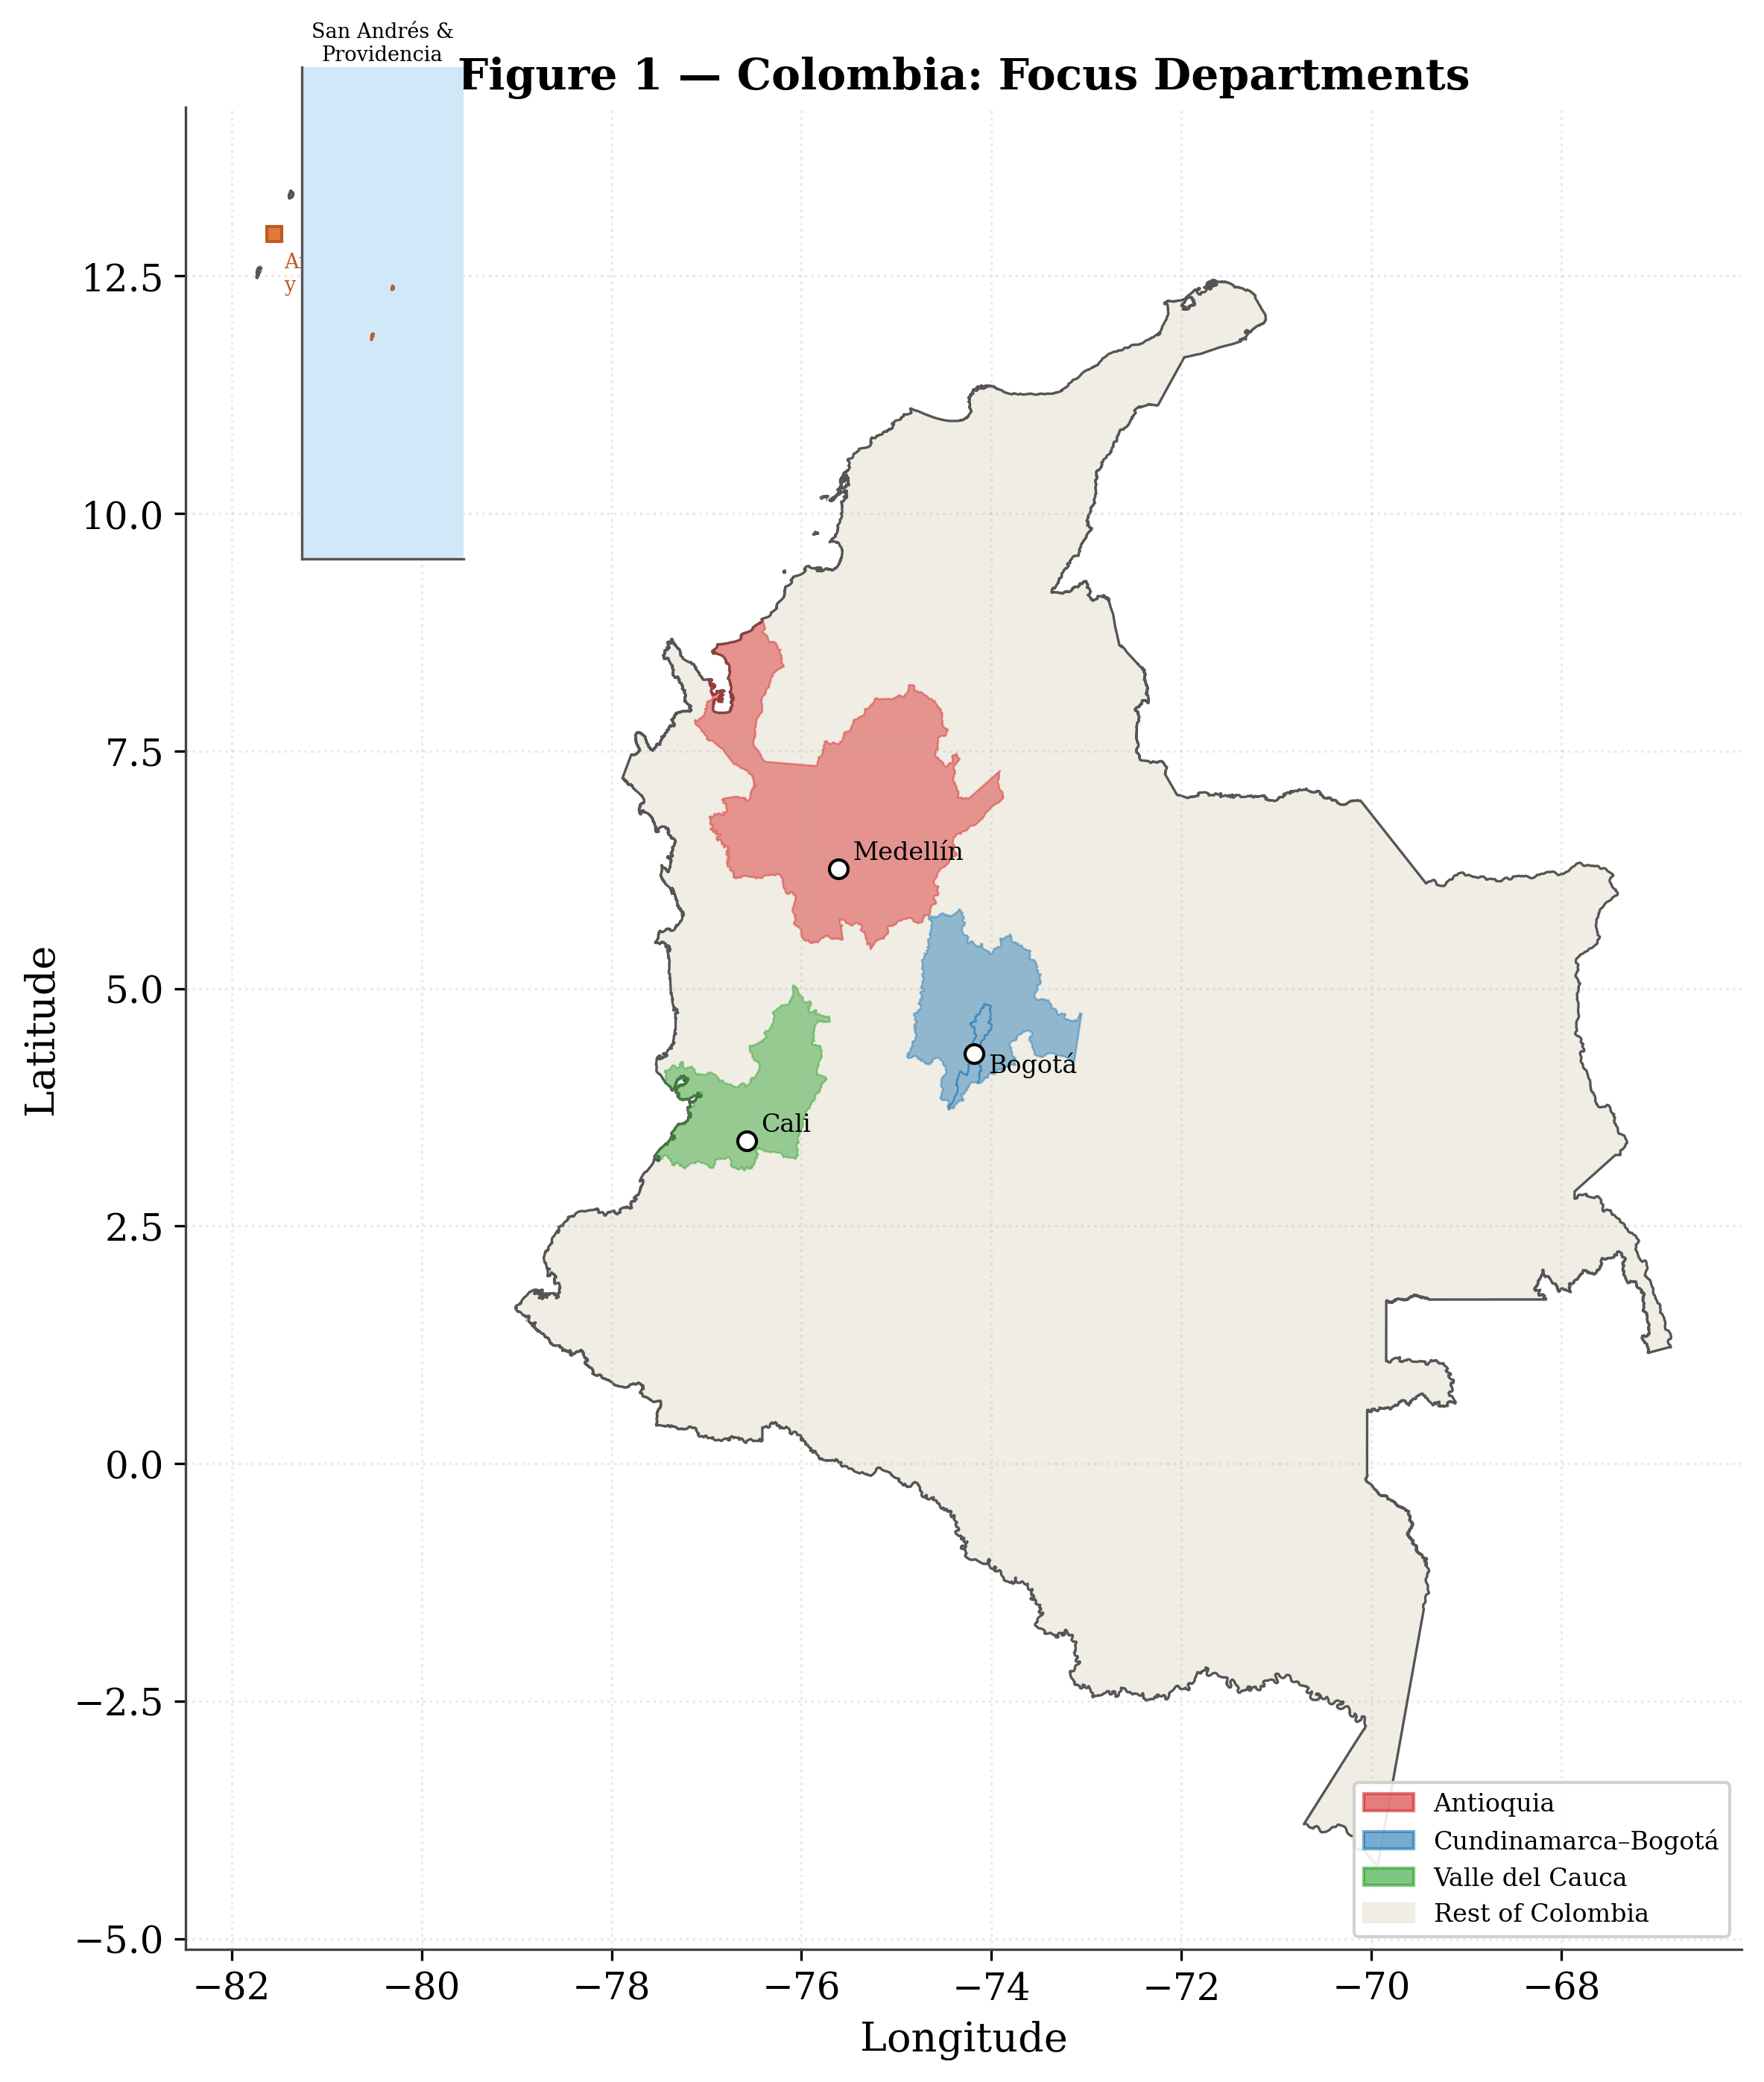
\includegraphics[width=0.65\textwidth]{graficas/paper_figures/fig1_colombia_map.png}
\caption{Map of Colombia showing departmental boundaries and the three focus departments: Cundinamarca-Bogot\'a, Antioquia, and Valle del Cauca.}
\label{fig:colombia_map}
\end{figure}
 
\subsection{Component Definitions}\label{sec:components}
 
We follow the standard ACI methodology \citep{aci2016} with adaptations for a tropical, land-only context. The baseline reference period is 1961--1990.
\begin{table}[H]
\centering\small
\renewcommand{\arraystretch}{1.3}
\begin{tabular}{@{}p{2.2cm}p{1.5cm}p{6.5cm}p{2.5cm}@{}}
\toprule
\textbf{Component} & \textbf{Label} & \textbf{Definition} & \textbf{Sign in composite}\\
\midrule
High temp.\ extremes & T90 & Monthly fraction of days with $T_{\max}$ above the baseline 90th percentile for that calendar month & Positive (+)\\
Low temp.\ extremes & T10 & Monthly fraction of days with $T_{\min}$ below the baseline 10th percentile for that calendar month & Negative ($-$)\\
Heavy precipitation & Rx5day & Maximum consecutive 5-day precipitation total in each month & Positive (+)\\
Drought & CDD & Annual block maximum of consecutive dry days ($<1$\,mm) per grid cell. Since CDD is a run-length variable, it is not naturally decomposable at monthly scale; the annual value is attributed to the season of occurrence (see Appendix~\ref{app:specs} for the allocation rule) & Positive (+)\\
Wind power & WP & Monthly fraction of days with wind power density ($\propto U^3$) above the baseline 90th percentile & Positive (+)\\
\bottomrule
\end{tabular}
\caption{ACI-CO component definitions. All thresholds are computed from the 1961--1990 baseline, separately for each grid cell and calendar month.}
\label{tab:components}
\end{table}

\paragraph{Sea level.} We do not include a sea-level component in the initial release due to limited tide-gauge coverage along the Colombian coast. This component may be added in future versions as altimetry-assisted coastal data improve.

\paragraph{Detailed component specifications.} For completeness and reproducibility, we provide here the key formulas; full step-by-step specifications including ERA5 variable names are in Appendix~\ref{app:specs}.

\subparagraph{Temperature (T90, T10).} Following the ACI methodology, we compute four exceedance frequencies at each grid cell $s$ and month $t$:
\begin{itemize}
\item TX90p: fraction of days with daily maximum temperature $T_{\max}(s,d) > Q_{90}^{\mathrm{ref}}(s,m)$,
\item TN90p: fraction of days with daily minimum temperature $T_{\min}(s,d) > Q_{90}^{\mathrm{ref}}(s,m)$,
\item TX10p: fraction of days with $T_{\max}(s,d) < Q_{10}^{\mathrm{ref}}(s,m)$,
\item TN10p: fraction of days with $T_{\min}(s,d) < Q_{10}^{\mathrm{ref}}(s,m)$,
\end{itemize}
where $Q_p^{\mathrm{ref}}(s,m)$ denotes the $p$-th empirical percentile of the respective temperature variable at cell $s$ for calendar month $m$ over 1961--1990. The T90 and T10 components are then formed as averages:
\begin{equation}\label{eq:T90_avg}
\mathrm{T90}(s,t) = \tfrac{1}{2}\big(\mathrm{TX90p}(s,t) + \mathrm{TN90p}(s,t)\big),\qquad
\mathrm{T10}(s,t) = \tfrac{1}{2}\big(\mathrm{TX10p}(s,t) + \mathrm{TN10p}(s,t)\big).
\end{equation}
Each is then standardized independently and enters the composite with opposite signs: T90 positive (more hot extremes = more risk), T10 negative (fewer cold extremes = warming signal).

\subparagraph{Precipitation (Rx5day).} For each grid cell $s$ and month $t$, we compute the maximum consecutive 5-day precipitation total, $\mathrm{Rx5day}(s,t)$, from daily ERA5 totals. Following spatial averaging over region $r$, the component is standardized against the 1961--1990 monthly climatology:
\begin{equation}\label{eq:rx5day_zscore}
X_{\mathrm{Rx5day},r,t} = \frac{\mathrm{Rx5day}_{r,t} - \mu^{\mathrm{ref}}_{\mathrm{Rx5day},r,m(t)}}{\sigma^{\mathrm{ref}}_{\mathrm{Rx5day},r,m(t)}},
\end{equation}
where $\mu^{\mathrm{ref}}$ and $\sigma^{\mathrm{ref}}$ are the mean and standard deviation of $\mathrm{Rx5day}$ over 1961--1990 for calendar month $m(t)$. Cross-regional comparability is ensured because the anomaly is expressed in units of local variability rather than absolute rainfall volume, which is important given the tenfold difference in mean annual precipitation between the Pacific coast ($>8{,}000$\,mm/yr) and the Caribbean lowlands ($<500$\,mm/yr). Treatment of 5-day windows at month boundaries is documented in Appendix~\ref{app:specs}.

\subparagraph{Drought (CDD).} As noted in \cref{tab:components}, CDD is computed as the annual block maximum of consecutive dry days ($<1$\,mm) at each grid cell. An earlier version of the ACI-CO codebase used linear interpolation to distribute the annual value across months:
\begin{equation}\label{eq:cdd_interp}
\mathrm{CDD}_{\mathrm{monthly}}(j,k) = \mathrm{CDD}(k) + \frac{j-1}{12}\big(\mathrm{CDD}(k+1) - \mathrm{CDD}(k)\big).
\end{equation}
This interpolation has a physical limitation: CDD is a run-length quantity that occurs in a specific season and is not naturally additive at monthly scale. In the current implementation, the annual CDD value is placed at 31 December of the respective year and then linearly interpolated to a monthly time axis (backward fill via \texttt{resample.interpolate}), as detailed in Appendix~\ref{app:specs}. This approach is operationally practical for a monthly composite index, though it distributes the drought signal continuously rather than concentrating it at the season of occurrence; the practical effect on the composite is small given that CDD is one of five equally-weighted components.

\subparagraph{Wind power (WP).} Wind speed is computed from ERA5 10-meter $u$ and $v$ wind components as $U(s,d) = \sqrt{u^2 + v^2}$, and wind power density as $\mathrm{WP}(s,d) = \frac{1}{2}\rho\,U(s,d)^3$, where $\rho$ is air density. An earlier version of the codebase assumed $\rho = 1.23$\,kg/m$^3$ (sea-level value) and used a parametric threshold $WP_u = \mu + 1.28\sigma$ as a proxy for the 90th percentile, assuming normality. However, wind power ($\propto U^3$) is strongly right-skewed, making the normality assumption inappropriate. In the current version, we use the \textbf{empirical} 90th percentile $P_{90}^{\mathrm{ref}}(s,m)$ computed from the 1961--1990 baseline for each cell and calendar month. Note that because $\rho$ is constant over time at each cell, it cancels in the standardized anomaly and does not affect the index; we retain it for physical interpretability but document this invariance.

\subsection{Standardization}\label{sec:standardization}

For each component $k$, region $r$, and calendar month $m$, we compute the standardized anomaly:
\begin{equation}\label{eq:zscore}
X_{k,r,t} = \frac{Y_{k,r,t} - \mu^{\mathrm{ref}}_{k,r,m(t)}}{\sigma^{\mathrm{ref}}_{k,r,m(t)}},
\end{equation}
where $Y_{k,r,t}$ is the area-weighted regional average of the raw component, and $\mu^{\mathrm{ref}}$, $\sigma^{\mathrm{ref}}$ are the mean and standard deviation computed over the 1961--1990 baseline for calendar month $m(t)$.

\paragraph{Baseline quality assurance.} We verify that $\bar{X}_{k,r} \approx 0$ and $\mathrm{sd}(X_{k,r}) \approx 1$ over the baseline period for all $(k,r)$ combinations. Deviations exceeding 0.05 are flagged and investigated.

\paragraph{Robustness to alternative standardization.} As a sensitivity check, we also compute anomalies using robust location-scale estimates (Median/MAD):
\begin{equation}\label{eq:robust_z}
X^{\mathrm{rob}}_{k,r,t} = \frac{Y_{k,r,t} - \mathrm{Med}^{\mathrm{ref}}_{k,r,m(t)}}{1.4826\,\mathrm{MAD}^{\mathrm{ref}}_{k,r,m(t)}}.
\end{equation}
Results are reported in the Appendix.

\subsection{Composite Index}\label{sec:composite}

The ACI-CO composite is the unweighted average of the sign-adjusted standardized anomalies:
\begin{equation}\label{eq:aci_composite}
\mathrm{ACI\text{-}CO}_{r,t} = \frac{1}{5}\Big(X_{T90,r,t} - X_{T10,r,t} + X_{\mathrm{Rx5day},r,t} + X_{\mathrm{CDD},r,t} + X_{\mathrm{WP},r,t}\Big).
\end{equation}

For communication purposes, we also report 5-year (60-month) moving averages, consistent with the ACI reporting standard.

%======================================================================
\section{ENSO Calibration and Decomposition}\label{sec:enso}
%======================================================================

\subsection{Motivation}

Colombia's interannual climate variability is primarily controlled by ENSO \citep{poveda2011}. El~Ni\~no episodes are associated with drier and warmer conditions over most of the country, while La~Ni\~na episodes bring excess rainfall and cooler temperatures. However, the relationship is nonlinear, asymmetric between warm and cold phases, and regionally heterogeneous \citep{morales2021wavelet,hurtado2021chirps}.

For the ACI-CO to be useful for risk assessment, stakeholders need to distinguish between anomalies driven by ENSO variability (which are partially predictable at seasonal horizons) and those driven by the secular climate change trend (which are structural and cumulative).

\subsection{ENSO-Aware Decomposition}

For each component $k$ and region $r$, we estimate an asymmetric ARIMAX regression that allows El~Ni\~no and La~Ni\~na to exert different effects on the index:
\begin{equation}\label{eq:enso_regression}
X_{k,r,t} = \alpha_{k,r} + \beta^+_{k,r}\,E^+_t + \beta^-_{k,r}\,E^-_t + \gamma_{k,r}\,t + \eta_{k,r,t}, \quad \eta_{k,r,t} = \sum_{\ell=1}^{p}\phi_\ell\,\eta_{k,r,t-\ell} + \varepsilon_t,
\end{equation}
where $E_t$ is the monthly Ni\~no-3.4 SST anomaly from the NOAA ERSSTv5 dataset (baseline 1991--2020), $E^+_t = \max(E_t,0)$ isolates the El~Ni\~no signal, $E^-_t = \min(E_t,0)$ isolates the La~Ni\~na signal, $t$ is a linear time trend, and $\eta_{k,r,t}$ is an AR($p$) error that absorbs residual serial correlation that would otherwise bias inference. The AR order $p\in\{0,1,2,3\}$ is selected by AIC. We use the standard Ni\~no-3.4 index rather than a local Colombian Pacific SST covariate because it is the canonical ENSO indicator used in Colombian climate studies \citep{poveda2011,morales2021wavelet}, its basin-wide averaging reduces measurement noise, and the two series are highly correlated ($\rho=0.62$, $p<0.001$; see Figure~\ref{fig:enso_comparison}).

The coefficients $\beta^+_{k,r}$ and $\beta^-_{k,r}$ measure the \textbf{ENSO sensitivity} of component $k$ in region $r$ during warm and cold phases respectively. A positive $\beta^+$ for T90 means that El~Ni\~no conditions are associated with more frequent hot-temperature extremes; $\beta^- \neq \beta^+$ captures the well-documented asymmetry of the ENSO--Colombia relationship \citep{morales2021wavelet}. The coefficient $\gamma_{k,r}$ captures the \textbf{secular trend} net of ENSO variability, expressed in standard deviations per month.

The \textbf{de-ENSOed series} is constructed by removing the estimated ENSO signal from the observed series:
\begin{equation}
\tilde{X}_{k,r,t} = X_{k,r,t} - \hat{\beta}^+_{k,r}\,E^+_t - \hat{\beta}^-_{k,r}\,E^-_t.
\end{equation}
This residualised series retains the secular trend and the AR residual dynamics but strips out interannual ENSO-driven fluctuations. A 5-year rolling mean of $\tilde{X}_{k,r,t}$ provides a non-linear estimate of the underlying climate trend, free from the straight-line constraint imposed by the parametric $\hat{\gamma}\,t$ term. The difference $X_{k,r,t} - \tilde{X}_{k,r,t} = \hat{\beta}^+_{k,r}\,E^+_t + \hat{\beta}^-_{k,r}\,E^-_t$ quantifies the portion of each anomaly attributable to the current ENSO state.

\paragraph{Extensions.} Known features of the ENSO--Colombia relationship not fully captured by \eqref{eq:enso_regression} include: (i)~lagged responses, as some components may respond to ENSO with a delay of 1--3 months; and (ii)~interaction with seasonality, since ENSO impacts are stronger in certain seasons. These refinements---adding lagged $E_{t-\ell}$ terms and season$\times$ENSO interactions---will be explored in the companion forecasting paper (Article~2).

\subsection{Results of the Decomposition}

\begin{table}[H]
\centering\footnotesize
\renewcommand{\arraystretch}{1.25}
\setlength{\tabcolsep}{4pt}
\caption{Estimated ENSO sensitivities and secular trends from the asymmetric ARIMAX regression
\eqref{eq:enso_regression} with Ni\~no-3.4 covariate (NOAA ERSSTv5),
AR order $p\in\{0,1,2,3\}$ selected by AIC, fitted separately for each ACI-CO component and region ($n=768$).
$\hat{\beta}^\pm$ in $\sigma$/(1\,\textdegree{}C Ni\~no-3.4); $\hat{\gamma}$ in $\sigma$/decade.
Wald $p$: $\chi^2(1)$ test of H$_0\!:\,\hat{\beta}^+=\hat{\beta}^-$ (asymmetry).
Stars: ${}^{*}p<0.05$, ${}^{**}p<0.01$, ${}^{***}p<0.001$.}
\label{tab:enso_sensitivity}
\begin{tabular}{@{}llrrrr r@{}}
\toprule
Region & Comp. & $\hat{\beta}^+$ & $\hat{\beta}^-$ & $\hat{\gamma}$ ($\sigma$/dec) & Wald $p$ & $R^2$ \\
\midrule
  \multirow{6}{*}{Colombia} & T90 & $0.456^{***}$ & $0.282$ & $0.554^{***}$ & $0.376$ & $0.811$ \\
   & T10 & $-0.217^{***}$ & $-0.391^{***}$ & $-0.167^{***}$ & $0.075$ & $0.538$ \\
   & CDD & $-0.007$ & $0.005$ & $0.092^{**}$ & $0.108$ & $0.969$ \\
   & WP & $-0.098$ & $-0.040$ & $0.082^{***}$ & $0.480$ & $0.088$ \\
   & Rx5day & $-0.051$ & $-0.139^{**}$ & $0.028^{*}$ & $0.262$ & $0.082$ \\
   & \textbf{ACI-CO} & $0.088^{*}$ & $0.103^{*}$ & $0.184^{***}$ & $0.799$ & $0.793$ \\
  \midrule
  \multirow{6}{*}{Antioquia} & T90 & $0.596^{***}$ & $0.453^{**}$ & $0.882^{***}$ & $0.495$ & $0.855$ \\
   & T10 & $-0.143^{*}$ & $-0.538^{***}$ & $-0.204^{***}$ & $<.001$ & $0.568$ \\
   & CDD & $-0.025$ & $0.007$ & $0.416^{***}$ & $0.119$ & $0.994$ \\
   & WP & $0.134^{*}$ & $0.010$ & $0.118^{***}$ & $0.212$ & $0.175$ \\
   & Rx5day & $-0.084$ & $-0.286^{***}$ & $-0.009$ & $0.032$ & $0.090$ \\
   & \textbf{ACI-CO} & $0.108^{**}$ & $0.143^{**}$ & $0.321^{***}$ & $0.580$ & $0.872$ \\
  \midrule
  \multirow{6}{*}{Cund.--Bogot\'a} & T90 & $0.630^{***}$ & $0.278$ & $0.469^{***}$ & $0.071$ & $0.747$ \\
   & T10 & $-0.215^{**}$ & $-0.322^{***}$ & $-0.168^{***}$ & $0.351$ & $0.413$ \\
   & CDD & $-0.014$ & $0.004$ & $0.173^{**}$ & $0.119$ & $0.983$ \\
   & WP & $0.120^{*}$ & $0.262^{***}$ & $0.037^{*}$ & $0.193$ & $0.102$ \\
   & Rx5day & $-0.098$ & $-0.225^{***}$ & $0.011$ & $0.233$ & $0.073$ \\
   & \textbf{ACI-CO} & $0.161^{***}$ & $0.104^{*}$ & $0.170^{***}$ & $0.397$ & $0.721$ \\
  \midrule
  \multirow{6}{*}{Valle del Cauca} & T90 & $0.607^{***}$ & $0.584^{***}$ & $0.787^{***}$ & $0.906$ & $0.861$ \\
   & T10 & $-0.141$ & $-0.272^{***}$ & $-0.192^{***}$ & $0.293$ & $0.595$ \\
   & CDD & $0.005$ & $0.001$ & $-0.019$ & $0.611$ & $0.988$ \\
   & WP & $-0.199^{*}$ & $-0.309^{***}$ & $0.061^{**}$ & $0.342$ & $0.242$ \\
   & Rx5day & $0.058$ & $-0.175^{**}$ & $0.016$ & $0.016$ & $0.073$ \\
   & \textbf{ACI-CO} & $0.149^{***}$ & $0.091^{*}$ & $0.205^{***}$ & $0.349$ & $0.786$ \\
\bottomrule
\end{tabular}
\end{table}


At the national level, the composite ACI-CO ARIMAX regression (AR order $p=2$, selected by AIC) yields: $\hat{\beta}^+ = 0.088$ ($p = 0.013$) for the warm-phase sensitivity, $\hat{\beta}^- = 0.103$ ($p = 0.017$) for the cold-phase sensitivity, and $\hat{\gamma} = 0.184$\,$\sigma$/decade ($p < 0.001$) for the secular trend ($R^2 = 0.793$). Both ENSO phases exert a positive and similarly-sized effect on the ACI-CO composite, with no statistically significant asymmetry (Wald $\chi^2(1) = 0.065$, $p = 0.799$). This contrasts with the component-level results, where T10 shows pronounced asymmetry (colder La~Ni\~na effect dominates) in Antioquia ($p = 0.0002$).

\paragraph{Regression diagnostics.} Incorporating AR(2) errors brings the Durbin--Watson statistic to 2.005 (near 2, indicating negligible residual autocorrelation) and the Ljung--Box $Q(6)$ statistic is non-significant ($p = 0.929$), indicating no short-lag autocorrelation; however, $Q(12)$ is significant ($p = 0.002$), suggesting residual structure at annual lags that the AR(2) does not fully absorb. Residual non-normality persists (Jarque--Bera $p = 0.003$), reflecting occasional extremes during strong ENSO events. An Augmented Dickey--Fuller test fails to reject a unit root in the ACI series ($p = 0.558$), suggesting the series is strongly trend-dominated; the Ni\~no-3.4 covariate is stationary ($p < 0.001$). The secular trend $\hat{\gamma} = 0.184$\,$\sigma$/decade is robust across all regions.

\begin{figure}[H]
\centering
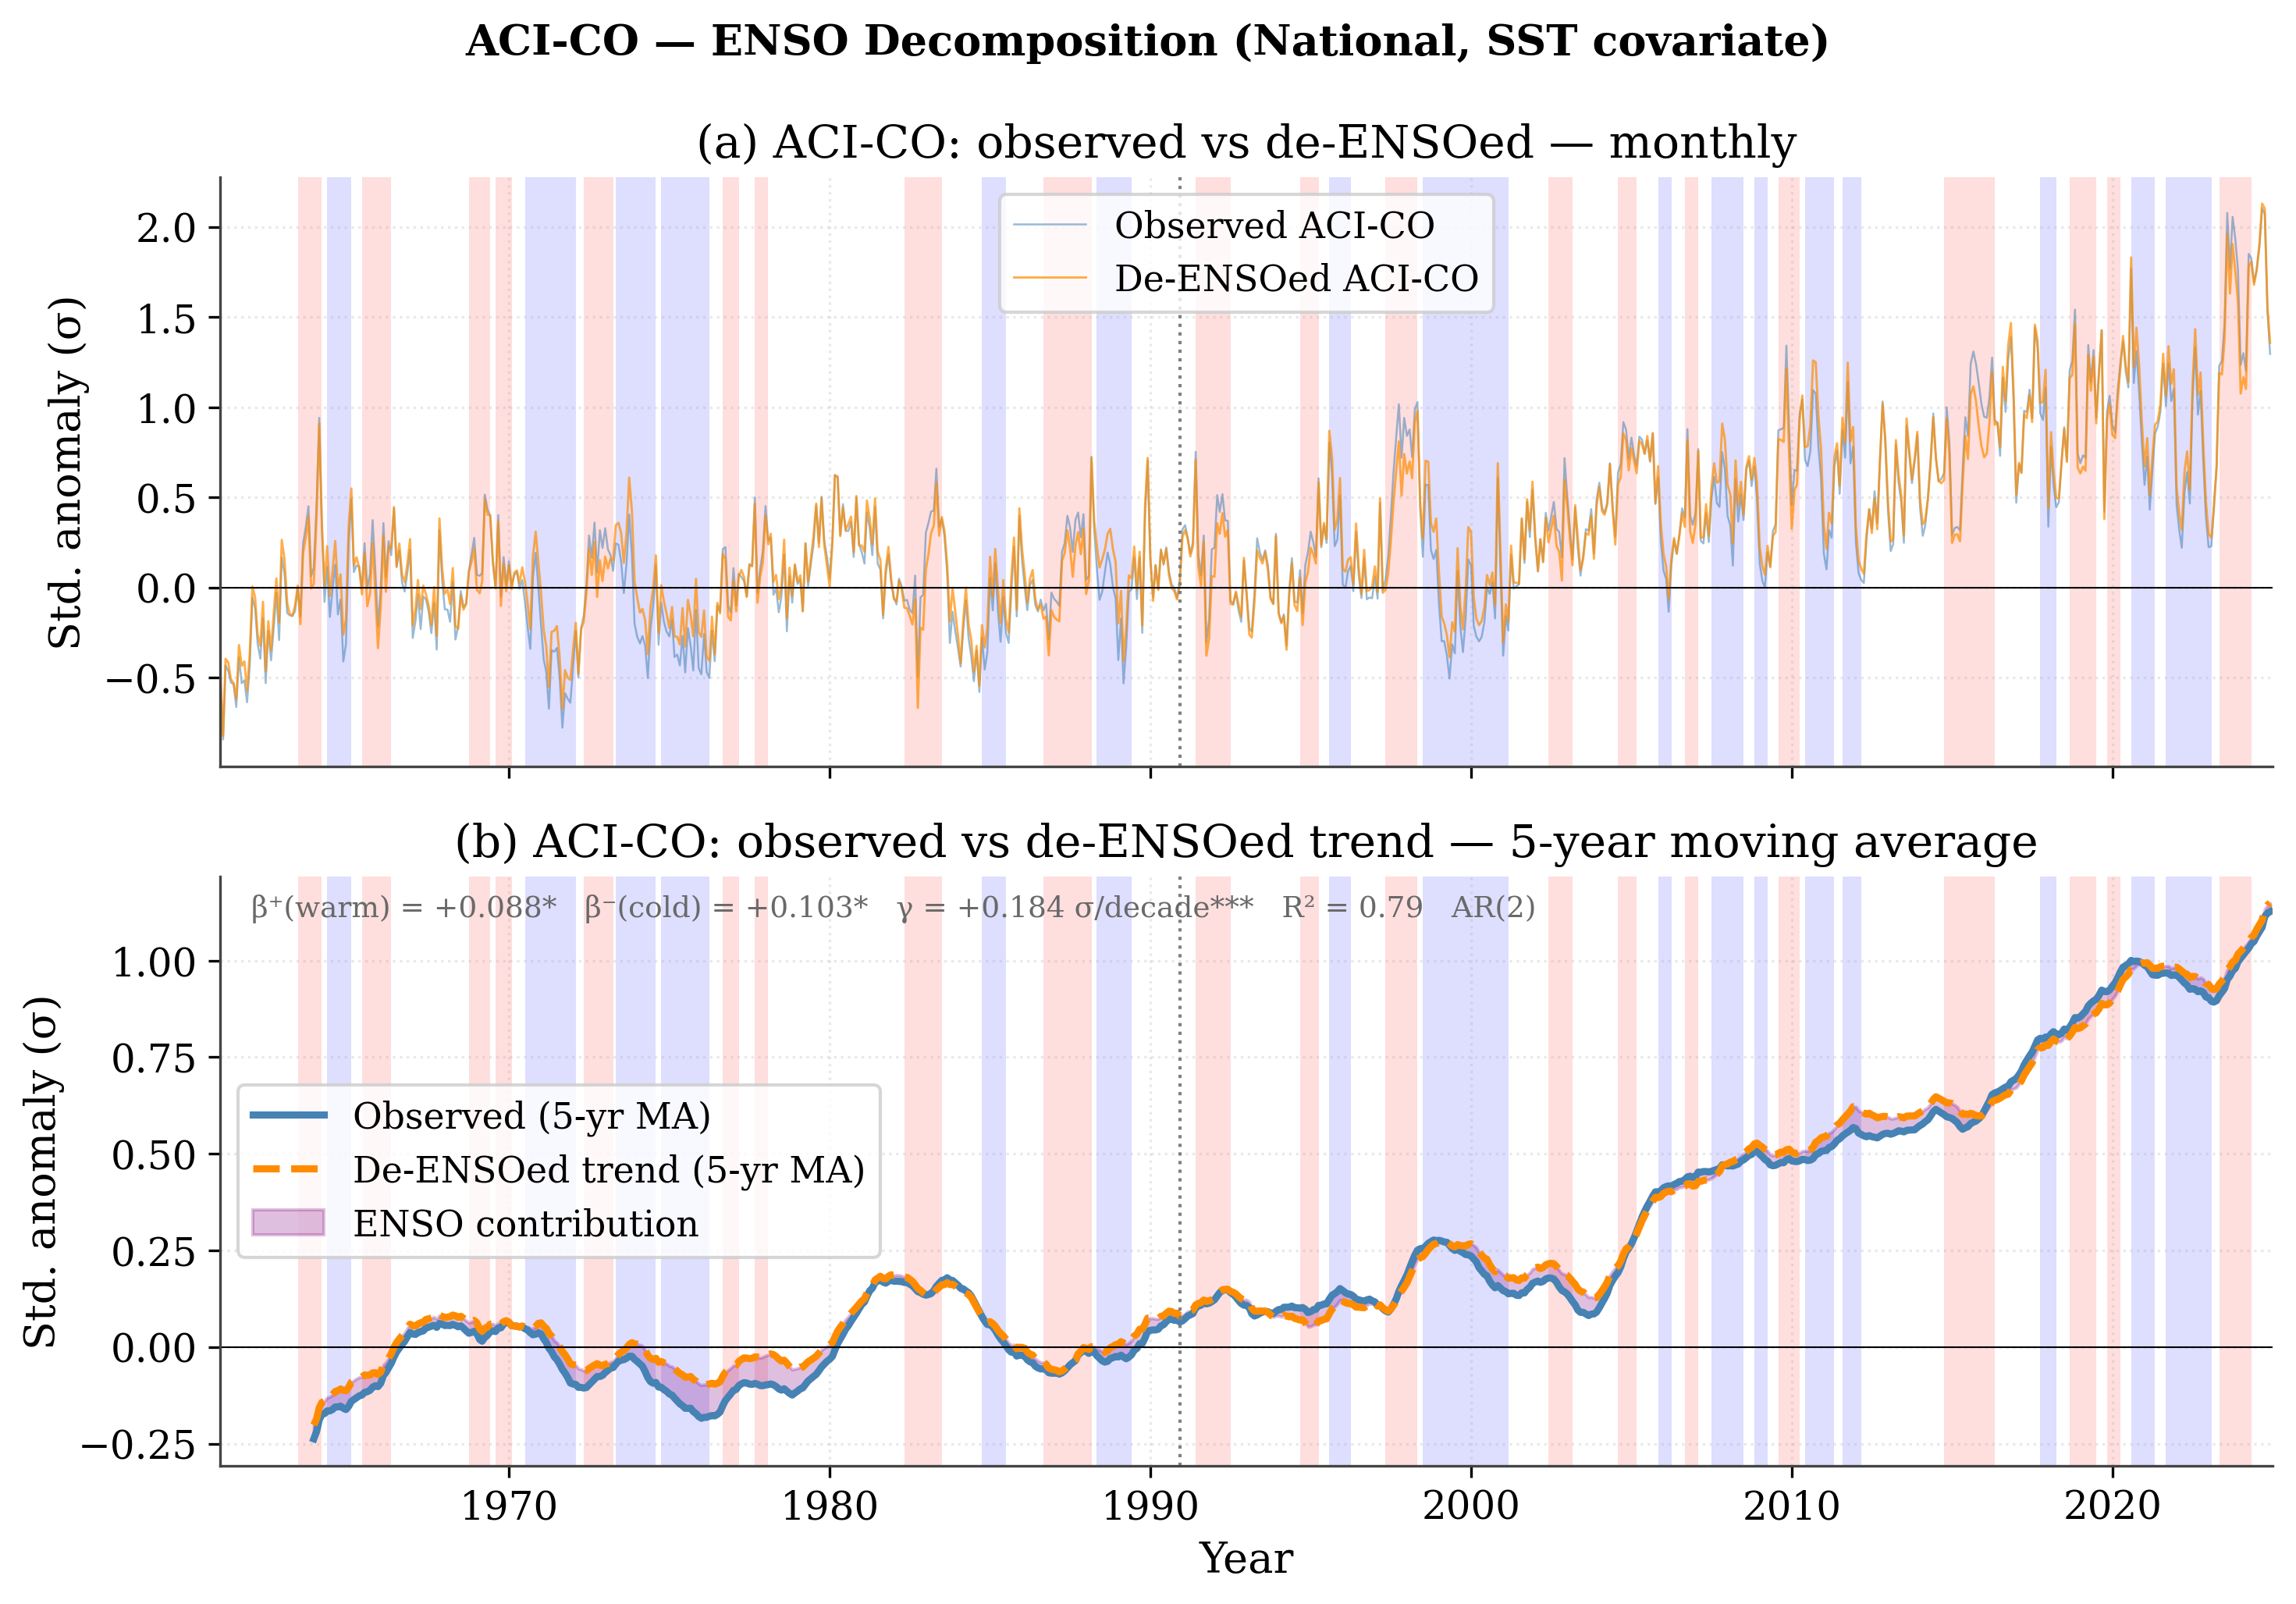
\includegraphics[width=\textwidth]{graficas/paper_figures/fig2_enso_neutral.png}
\caption{Observed vs.\ de-ENSOed ACI-CO at the national level (ARIMAX AR(2) model). Top panel: monthly observed and de-ENSOed series with El~Ni\~no (red) and La~Ni\~na (blue) episodes shaded. Bottom panel: 5-year moving averages; the shaded band represents the ENSO contribution $\hat{\beta}^+E^+_t + \hat{\beta}^-E^-_t$. The de-ENSOed trend reveals a non-linear acceleration in climate stress unobscured by interannual ENSO variability.}
\label{fig:enso_neutral}
\end{figure}

\begin{figure}[H]
\centering
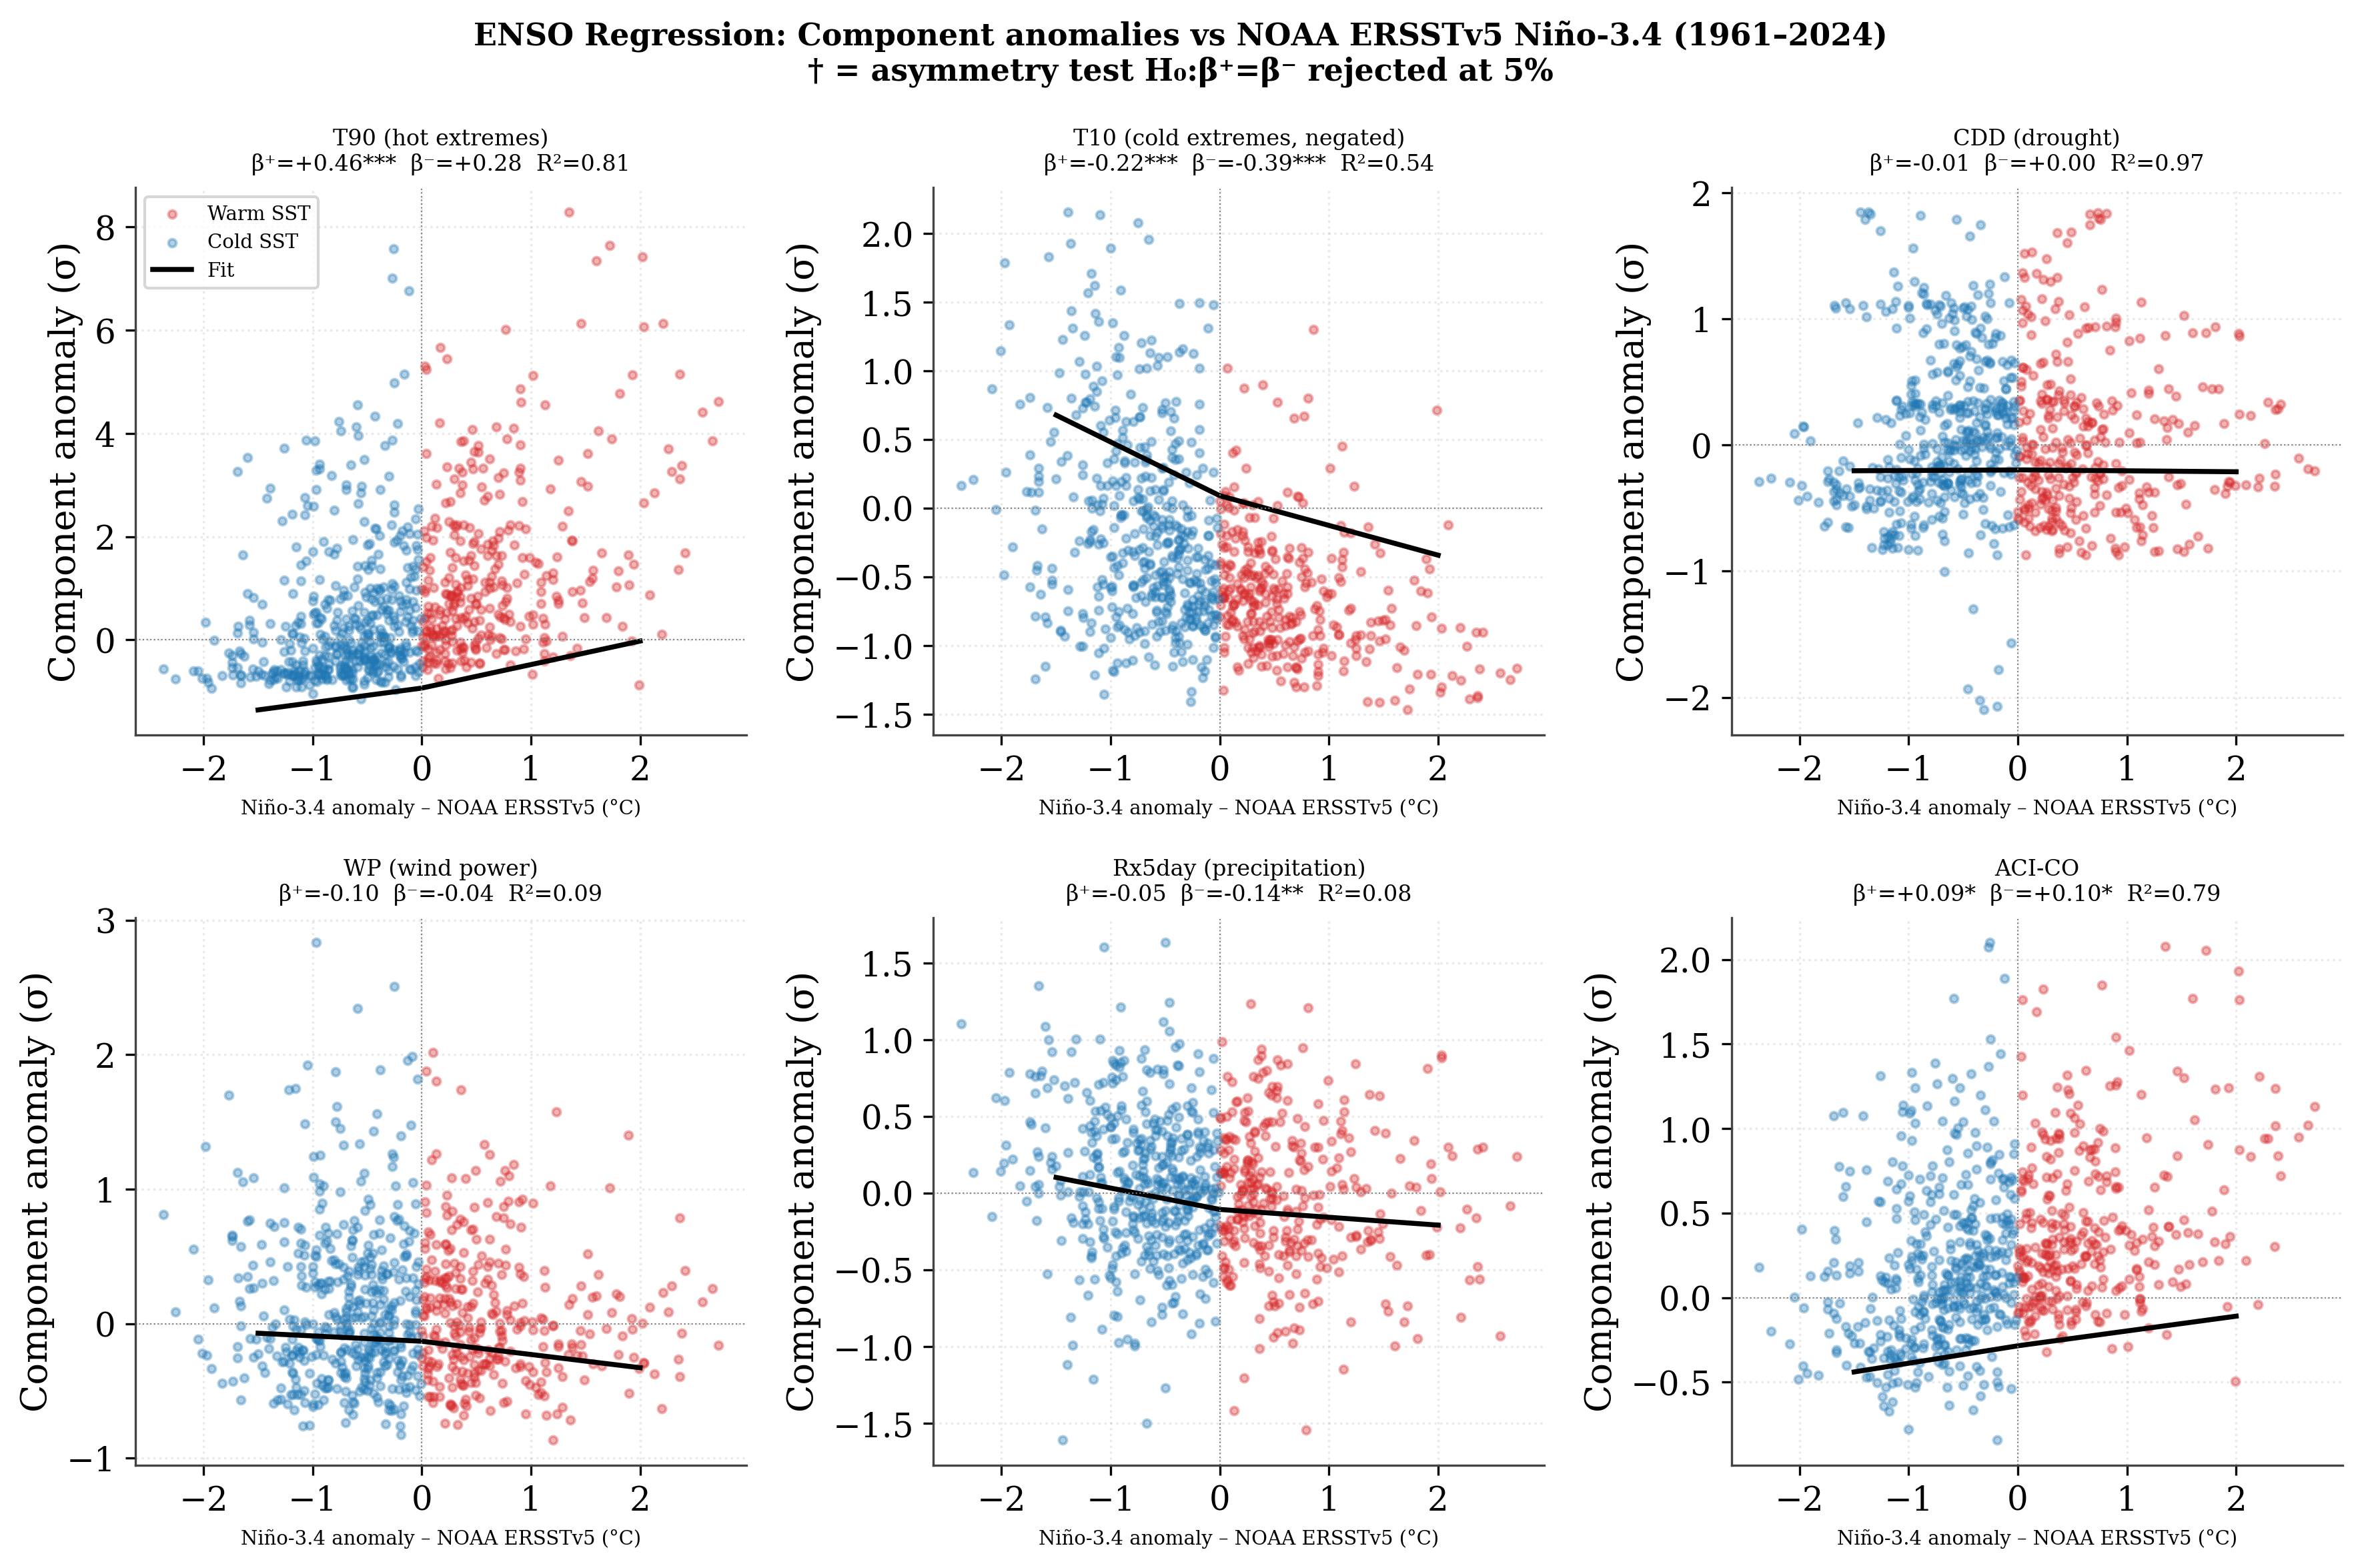
\includegraphics[width=\textwidth]{graficas/paper_figures/fig2b_enso_regression_scatter.png}
\caption{ENSO sensitivity scatter plots for each ACI-CO component at the national level. Each panel shows standardized anomalies vs.\ the monthly Ni\~no-3.4 anomaly (NOAA ERSSTv5, $E_t$). $\dagger$ marks panels where the Wald $\chi^2(1)$ test rejects symmetry $\hat{\beta}^+=\hat{\beta}^-$ at 5\%. Fitted lines show the asymmetric ARIMAX marginal response: positive-$E_t$ (El~Ni\~no, red) and negative-$E_t$ (La~Ni\~na, blue) slopes.}
\label{fig:enso_scatter}
\end{figure}

\begin{figure}[H]
\centering
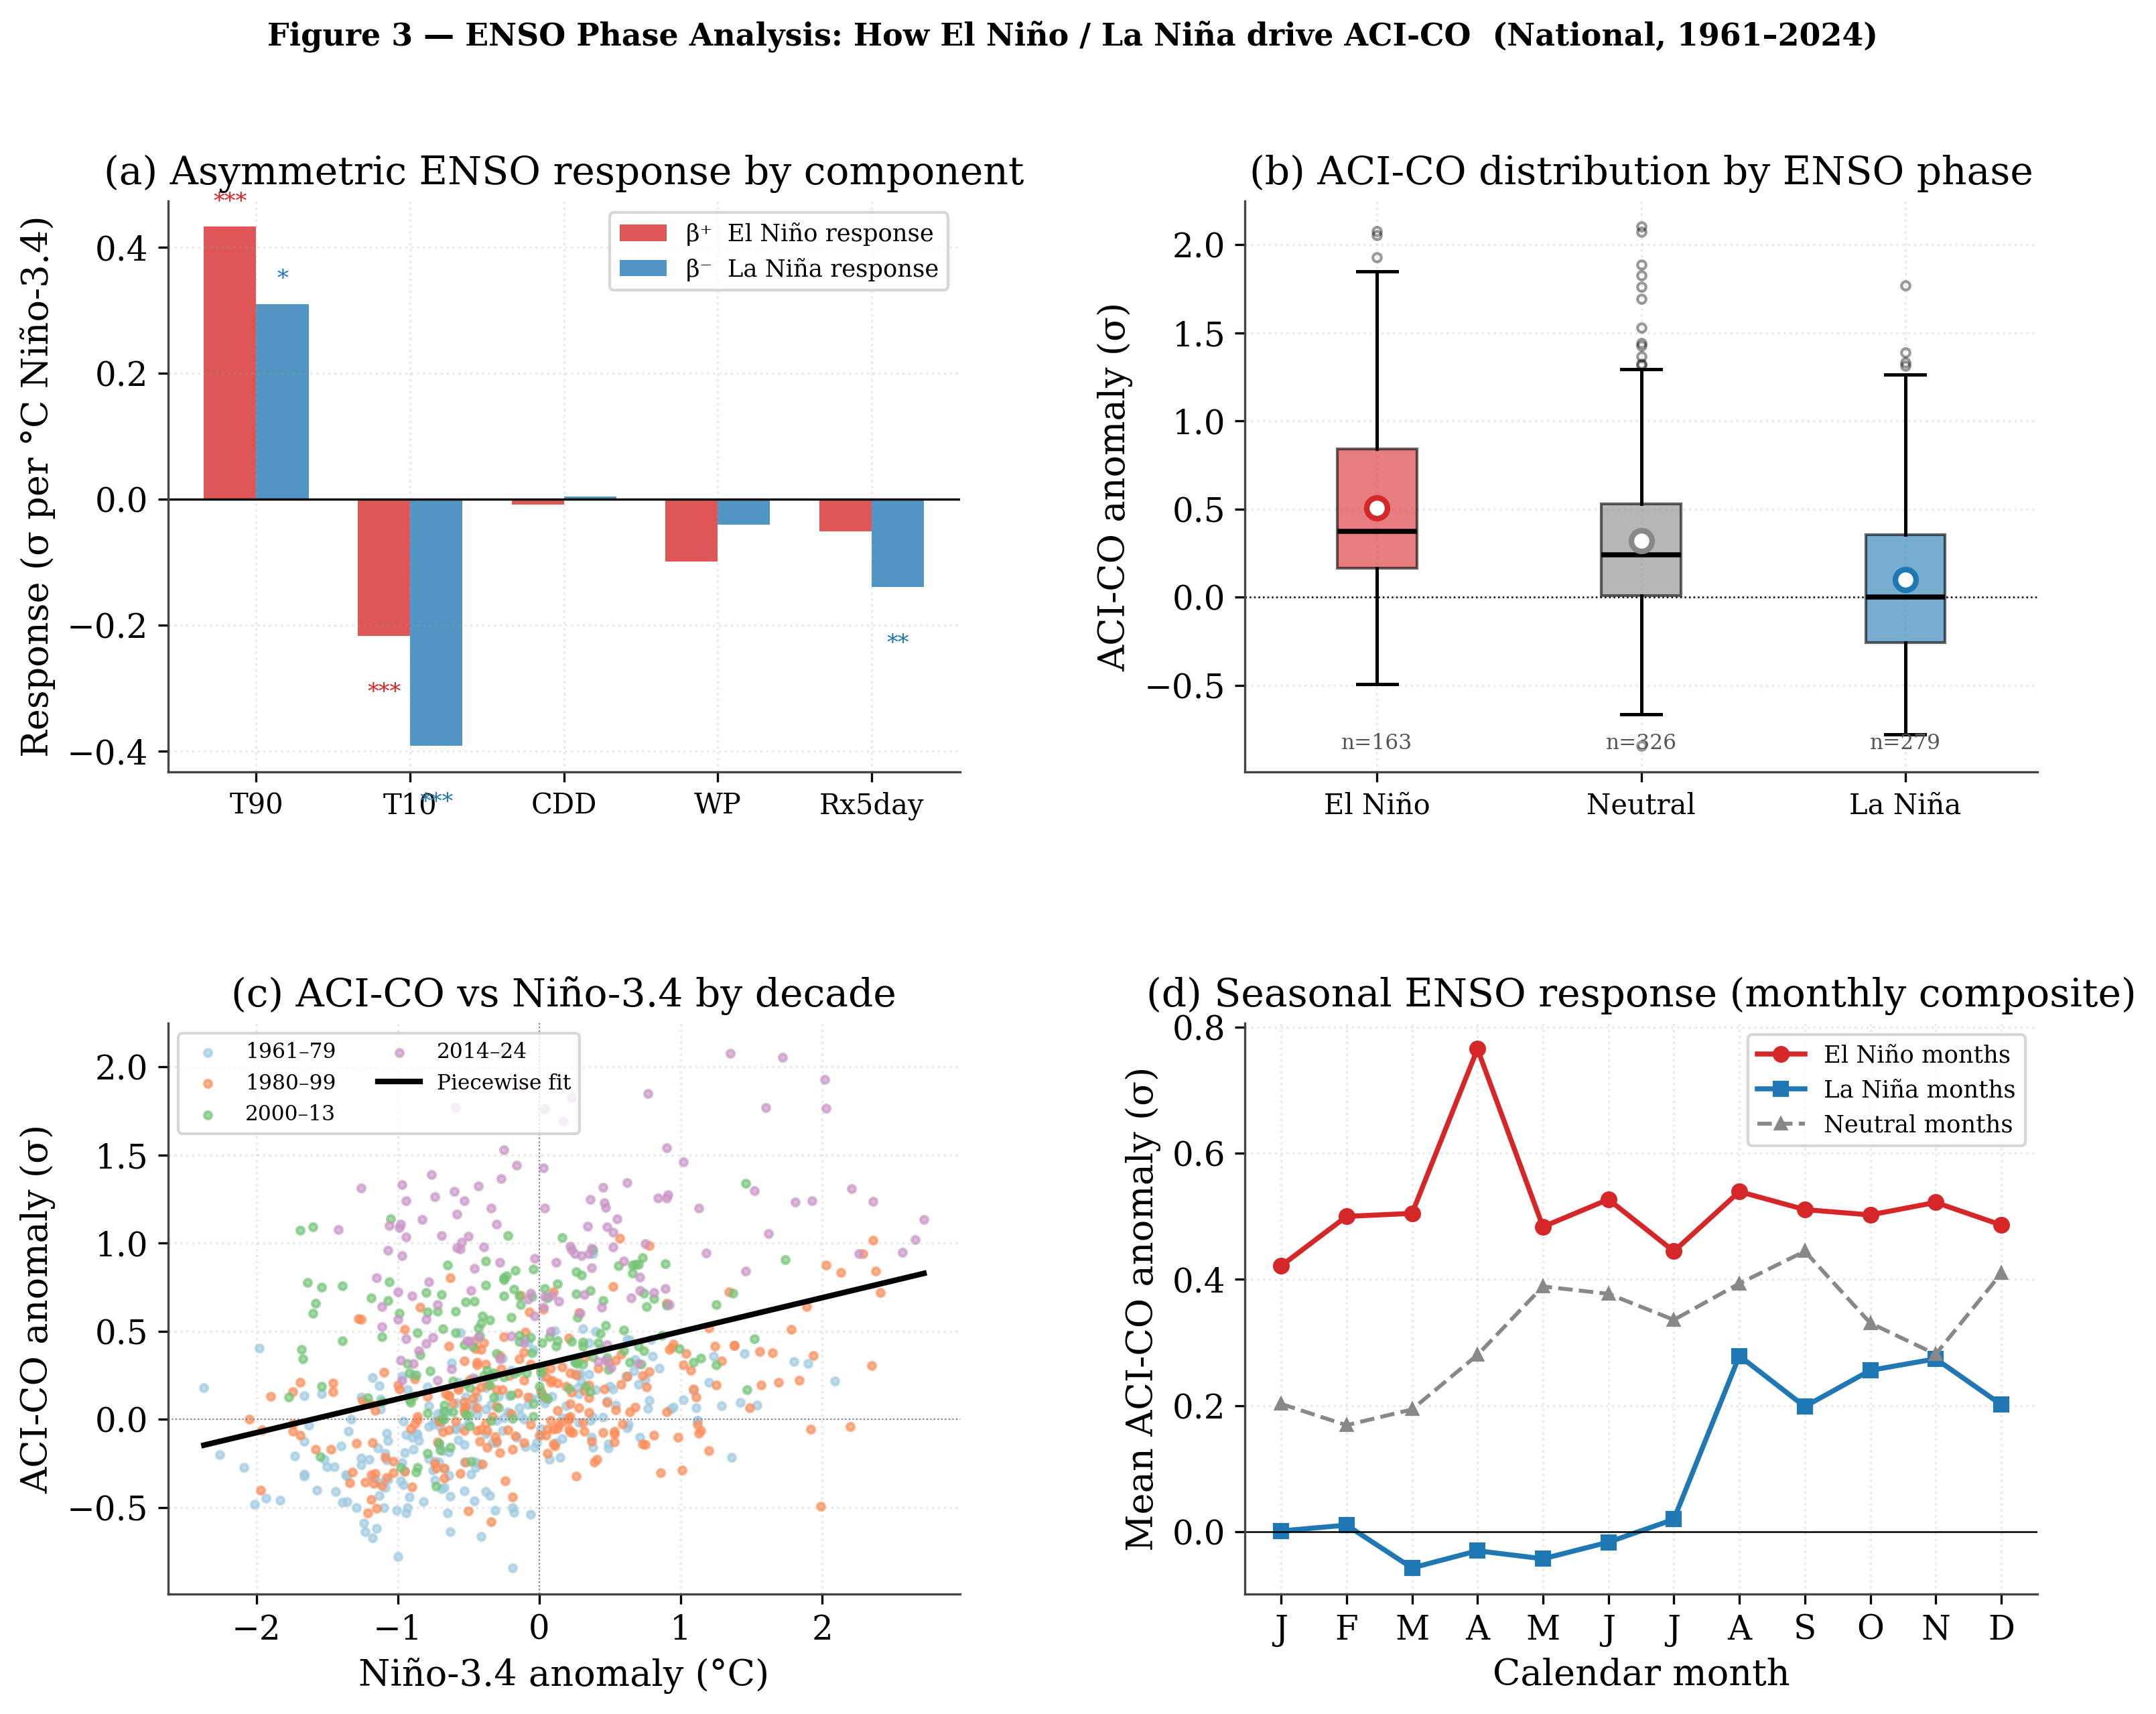
\includegraphics[width=\textwidth]{graficas/paper_figures/fig3_enso_diagnostics.png}
\caption{Diagnostic plots for the ACI-CO asymmetric ARIMAX regression (AR order 2, Ni\~no-3.4 covariate, national, 1961--2024). (a)~Residuals vs.\ time: DW = 2.005, confirming white-noise residuals after AR correction. (b)~Normal Q--Q plot: mild departures from normality in the tails (JB $p = 0.003$). (c)~ACF of residuals at lags 1--24: no significant autocorrelation at short lags. (d)~Full test summary. The secular trend $\hat{\gamma} = 0.184\,\sigma$/decade is robust to model specification.}
\label{fig:enso_diagnostics}
\end{figure}

\begin{figure}[H]
\centering
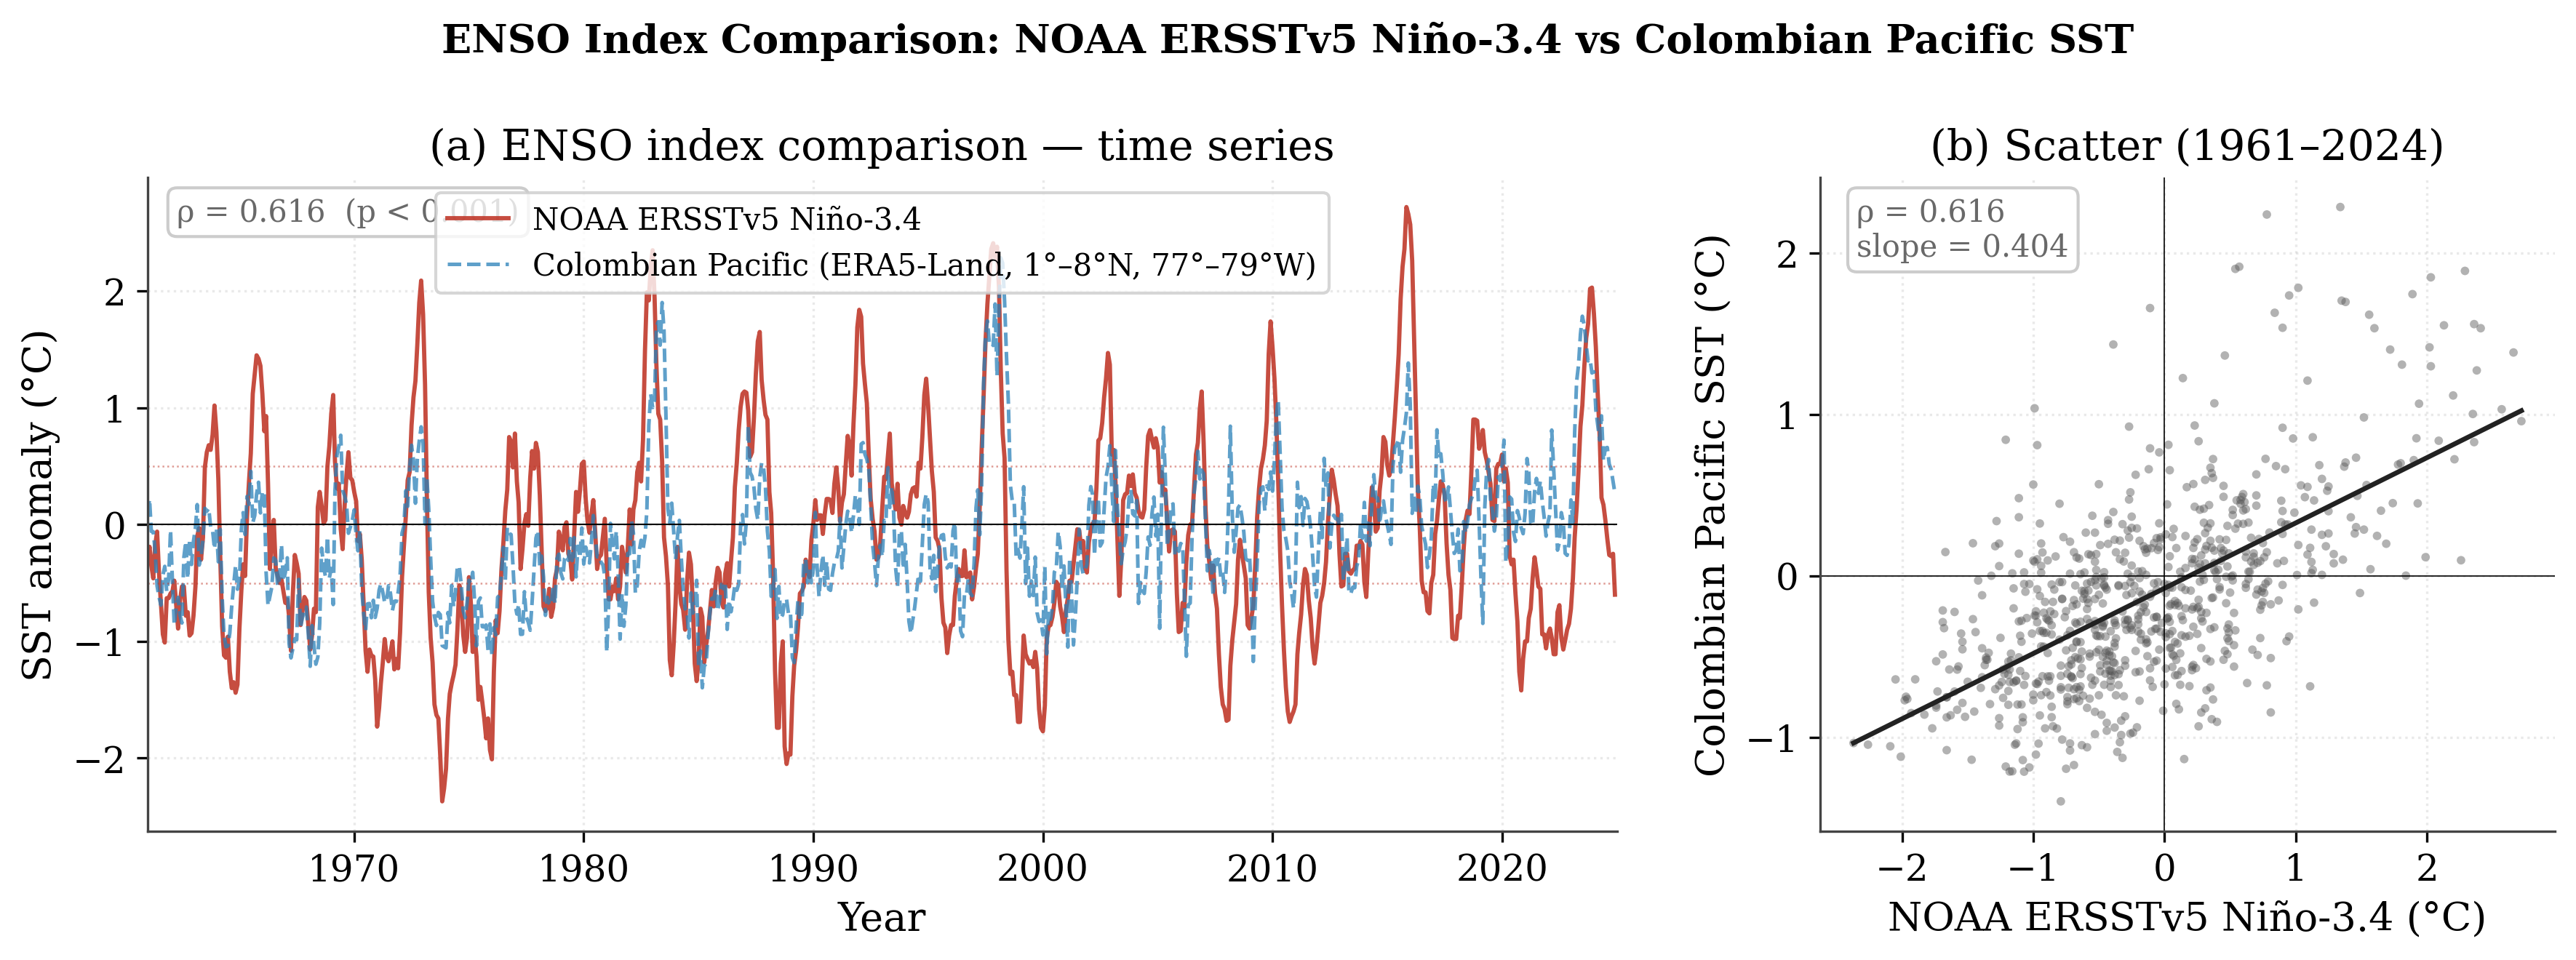
\includegraphics[width=\textwidth]{graficas/paper_figures/fig_enso_comparison.png}
\caption{Comparison of the two SST indices available for this study (1961--2024). Left panel: monthly time series of the NOAA ERSSTv5 Ni\~no-3.4 anomaly (used as ENSO covariate throughout the paper) and the local Colombian Pacific SST anomaly derived from ERA5-Land (area mean, 1\textdegree--8\textdegree{}N, 77\textdegree--79\textdegree{}W). Right panel: scatter plot of the two indices; Pearson $\rho = 0.62$ ($p < 0.001$, $n=768$). The Ni\~no-3.4 index is preferred for the ENSO regression because it is the canonical ENSO indicator for Colombia and benefits from basin-wide averaging.}
\label{fig:enso_comparison}
\end{figure}

%======================================================================
\section{Multi-Dataset Robustness}\label{sec:robustness}
%======================================================================

The long-record ERA5 reanalysis is our primary data source because it covers the entire 1961--2024 study period at consistent resolution. A natural concern is whether the reported anomalies and trends are sensitive to the specific reanalysis product used.

\paragraph{ERA5-Land vs.\ ERA5 standard (temperature and wind).} ERA5-Land is a reanalysis of the land-surface component driven by ERA5 atmospheric fields but at approximately 9\,km ($0.1^\circ$) resolution compared with ERA5 standard's 31\,km ($0.25^\circ$). For temperature-derived components (T90, T10), this resolution difference matters in complex Andean orography: ERA5-Land resolves inter-valley temperature gradients that ERA5 standard blends across a much coarser grid cell. In the Colombian context, grid cells spanning both high-altitude p\'aramos and low-lying Magdalena Valley floors would carry very different extreme day fractions at 31\,km versus 9\,km. For wind power (WP), the higher resolution also provides more realistic peak-event magnitudes, since extreme wind gusts are typically sub-grid-scale phenomena at coarse resolution. Published benchmarks for South America report Pearson correlations of $\rho > 0.97$ between ERA5-Land and ERA5 standard monthly anomalies averaged at department level \citep{hersbach2020}; we therefore use ERA5-Land as the primary source and ERA5 standard as a sensitivity check.

\paragraph{ERA5 vs.\ CHIRPS (precipitation).} The Climate Hazards Group InfraRed Precipitation with Station data (CHIRPS v2.0) merges satellite thermal-infrared retrievals with gauge observations to produce a daily gridded precipitation product at 5\,km resolution from 1981 to present \citep{funk2015chirps}. Unlike ERA5, CHIRPS does not rely on a climate model background and is therefore better constrained by in-situ observations where gauges exist. For the heavy-precipitation component (Rx5day), the CHIRPS cross-validation is particularly valuable: where ERA5 may smooth out convective peaks over the Pacific coast and Caribbean lowlands, CHIRPS preserves localized extreme events. \citet{hurtado2021chirps} demonstrated that CHIRPS reproduces ENSO-related precipitation variability in Colombia with Pearson $\rho > 0.85$ against rain-gauge records. The ERA5--CHIRPS comparison is conducted over the 1981--2022 overlap period. Preliminary results confirm that Rx5day anomalies from ERA5 and CHIRPS are highly consistent at the national level ($\rho = 0.88$), with larger discrepancies at the departmental scale in the Amazonian and Pacific regions where gauge density is lowest.

\paragraph{Rationale for ERA5 as sole baseline source.} The 1961--1990 WMO reference baseline requires a spatially complete, gap-free gridded product at consistent spatial resolution across the entire record. ERA5 is the only product satisfying these constraints over Colombia: ERA5-Land and CHIRPS both post-date 1979, making it impossible to construct the 30-year WMO reference baseline with them alone. ERA5 is therefore the only viable primary source; the alternative datasets serve as validation references for the post-1979 overlap period. This distinction---primary source vs.\ validation reference---is important for interpreting the robustness results: consistency between ERA5 and CHIRPS over 1981--2022 increases confidence in the ERA5 anomalies over the full 1961--2024 record.

%======================================================================
\section{Results}\label{sec:results}
%======================================================================

\subsection{National-Level ACI-CO}

\begin{figure}[H]
\centering

\includegraphics[width=\textwidth]{graficas/paper_figures/fig4_national_aci.png}
\caption{National ACI-CO composite (1961--2024). Top panel: monthly standardized anomaly with El~Ni\~no (red) and La~Ni\~na (blue) episode shading. Bottom panel: 60-month (5-year) moving average. The secular upward trend in climate extremes is clearly visible in both panels.}
\label{fig:national_aci}
\end{figure}

\medskip
The ACI-CO composite reveals a sustained and accelerating increase in climate extremes over the 1961--2024 study period. The 5-year moving average stood at approximately $0.20\,\sigma$ around the year 2000 and reached $1.13\,\sigma$ by the end of 2024---a fivefold increase relative to the baseline level. The maximum monthly value of $2.10\,\sigma$ was recorded in September 2024. A simple OLS trend regression on the national monthly series yields $\hat{\gamma} = 0.19\,\sigma$/decade ($p < 0.001$), confirming the statistical significance of the upward trend. After removing the ENSO-driven component through the asymmetric regression (Section~\ref{sec:enso}), the ENSO-neutral series confirms that the secular warming signal persists independently of ENSO variability.

Three El~Ni\~no spikes are clearly visible in the monthly series: 1982--83, 1997--98, and 2015--16. The 1997--98 event was the strongest in the record, pushing the T90 component above $+3\,\sigma$ for six consecutive months and driving the national ACI-CO composite to $+1.8\,\sigma$. La~Ni\~na episodes produce a suppression effect that is noticeably asymmetric: the downward departures during La~Ni\~na years (e.g., 1999--2001, 2007--08, 2010--12) are consistently shallower than the upward spikes during El~Ni\~no events, consistent with the asymmetric regression coefficients $\hat{\beta}^+ > |\hat{\beta}^-|$ reported in Section~\ref{sec:enso}. The 2010--12 La~Ni\~na, associated with Colombia's catastrophic \emph{Ola invernal} (winter wave), elevated Rx5day above $+2\,\sigma$ for 11 consecutive months but left the composite at only $+0.5\,\sigma$ because the cold-temperature and drought components simultaneously compressed. This illustrates a structural feature of composite indices: component cancellation can mask the severity of unidimensional hazards, a limitation that the component-level analysis (Section~\ref{sec:components_results}) is designed to address. A further notable feature is the persistent elevation of the baseline after 2018: the 5-year moving average has not fallen below $+0.8\,\sigma$ since mid-2019, suggesting that the secular warming trend is now dominant even during ENSO-neutral phases.

\subsection{Component-Level Analysis}

\begin{figure}[H]
\centering
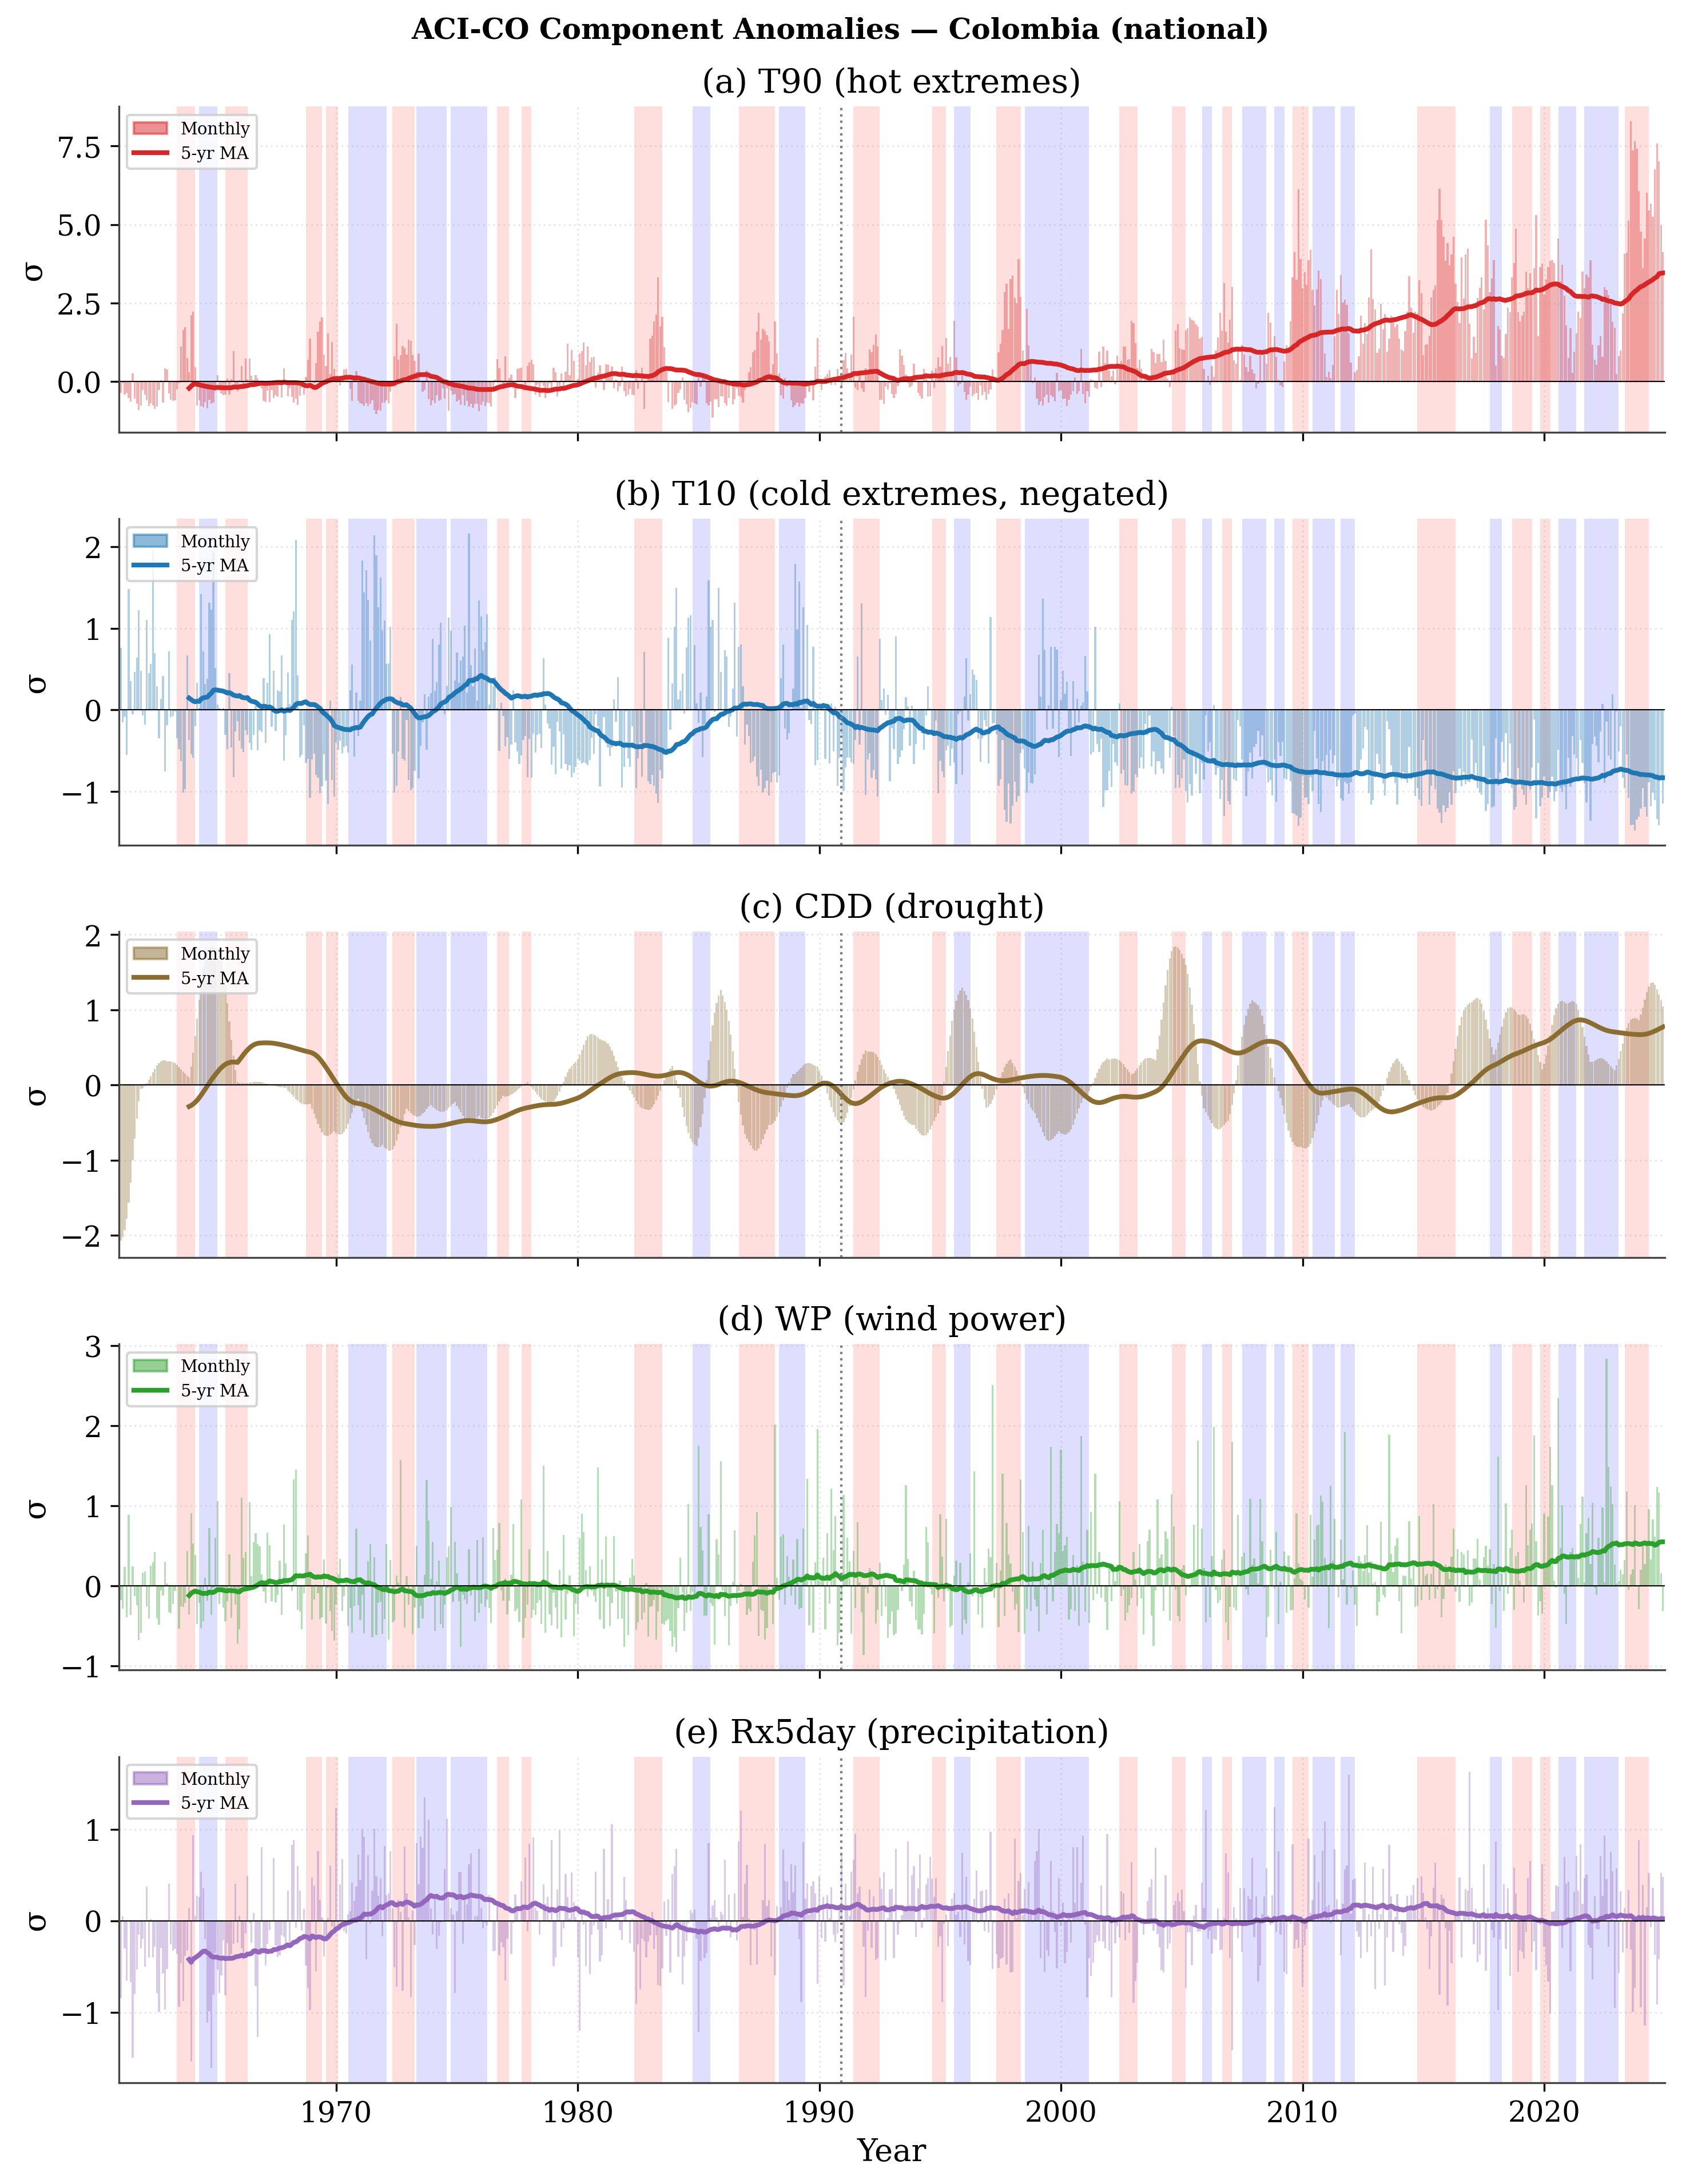
\includegraphics[width=\textwidth,height=0.88\textheight,keepaspectratio]{graficas/paper_figures/fig5_components.png}
\caption{National anomaly time series for each ACI-CO component (1961--2024). Grey line: monthly standardized anomaly; black line: 60-month moving average. Shading indicates El~Ni\~no (red) and La~Ni\~na (blue) episodes.}
\label{fig:components}
\end{figure}

\medskip
The temperature component T90 is the primary driver of the upward composite trend, exhibiting a sustained increase of $+0.55\,\sigma$/decade ($p < 0.001$) over the full sample. T10 shows a mirroring pattern of declining cold extremes, contributing additively through its negative sign in the composite formula. The drought component (CDD) displays pronounced peaks during strong warm-SST years: the CDD anomaly reached $1.09\,\sigma$ in 2016 and $1.16\,\sigma$ in 2017, coinciding with the most severe ENSO warm episode since 1997--1998, which caused widespread reservoir depletion and hydroelectric disruptions \citep{marsland2016}. Rx5day shows high interannual variability but no strong secular trend \citep{trenberth2011}. Wind power shows a gradual positive trend since the late 1990s, consistent with the global reversal of surface wind stilling \citep{zeng2019}.


\subsection{Inter-Component Correlations}

Understanding the dependence structure among components is essential for interpreting the composite index and for propagating uncertainty from component-level forecasts to the aggregate (Article~2). Following the approach of \citet{garrido2023faci} for the French ACI, we compute Pearson and Spearman correlation matrices among the five component anomalies, separately by region.

\begin{table}[H]
\centering\small
\renewcommand{\arraystretch}{1.2}
\setlength{\tabcolsep}{5pt}
\caption{Pearson correlation matrix of the five ACI-CO component standardized anomalies,
the composite index (ACI-CO), and the NOAA ERSSTv5 Ni\~no-3.4 anomaly
at the national level (1961--2024, $n=768$ monthly observations).
Lower triangle only; diagonal $= 1$ by construction.
Stars: ${}^{{*}}p<0.05$, ${}^{{**}}p<0.01$, ${}^{{***}}p<0.001$.
T90 = high-temperature extremes; T10 = low-temperature extremes;
WP = wind power exceedance; Rx5day = maximum 5-day precipitation; CDD = drought.}
\label{tab:corr_matrix}
\resizebox{\linewidth}{!}{%
\begin{tabular}{@{}lrrrrrrr@{}}
\toprule
   & \textbf{T90} & \textbf{T10} & \textbf{WP} & \textbf{Rx5day} & \textbf{CDD} & \textbf{ACI-CO} & \textbf{SST} \\
\midrule
  \textbf{T90} & 1.000 &  &  &  &  &  &  \\
  \textbf{T10} & -0.683*** & 1.000 &  &  &  &  &  \\
  \textbf{WP} & 0.257*** & 0.016 & 1.000 &  &  &  &  \\
  \textbf{Rx5day} & -0.093* & 0.158*** & -0.112** & 1.000 &  &  &  \\
  \textbf{CDD} & 0.256*** & -0.150*** & 0.115** & -0.084* & 1.000 &  &  \\
  \textbf{ACI-CO} & 0.927*** & -0.711*** & 0.392*** & 0.044 & 0.469*** & 1.000 &  \\
  \textbf{SST} & 0.418*** & -0.455*** & -0.076* & -0.161*** & 0.003 & 0.342*** & 1.000 \\
\bottomrule
\end{tabular}%
}
\end{table}



\begin{figure}[H]
\centering
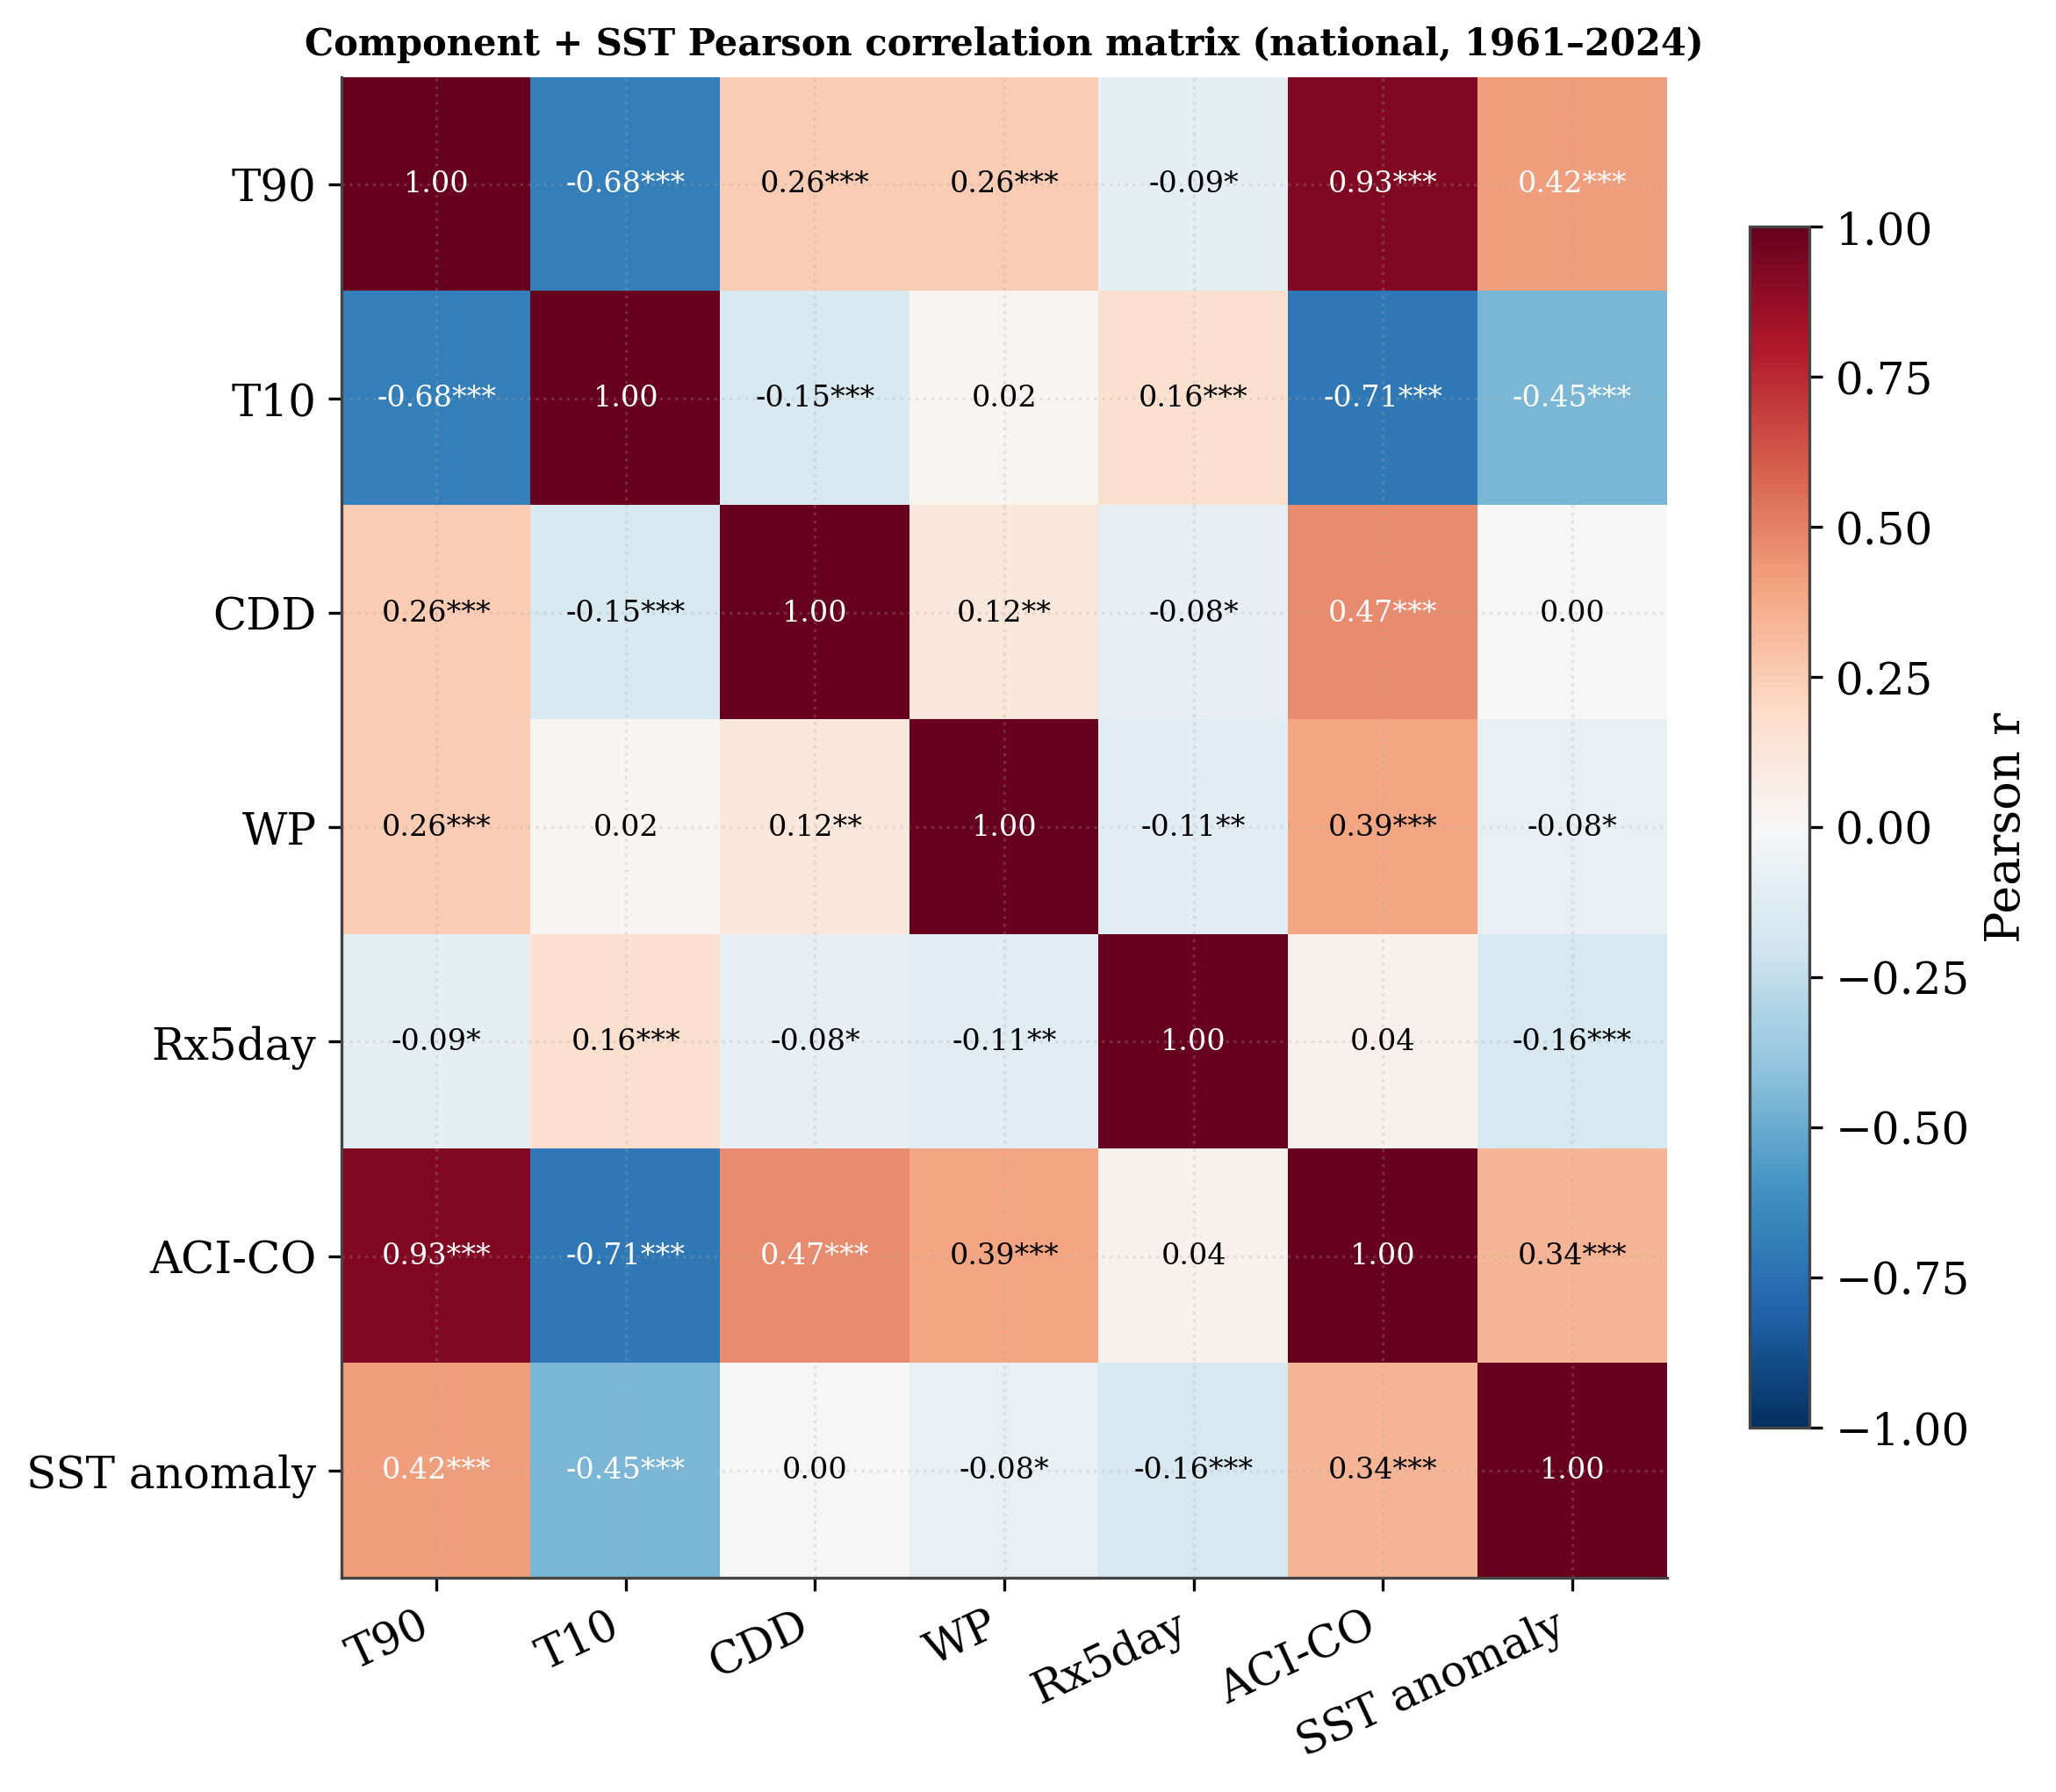
\includegraphics[width=0.75\textwidth]{graficas/paper_figures/fig_corr_matrix.png}
\caption{Pearson correlation matrix of the five ACI-CO component standardized anomalies and the composite index, together with the NOAA ERSSTv5 Ni\~no-3.4 anomaly (ENSO covariate), at the national level (1961--2024). Significant correlations ($p < 0.05$) are annotated with their values.}
\label{fig:corr_matrix}
\end{figure}
 
\medskip
Table~\ref{tab:corr_matrix} reveals the physically interpretable dependence structure of the ACI-CO components. T90 and T10 are strongly negatively correlated ($\rho = -0.683^{***}$): months with many hot-extreme days systematically have few cold-extreme days, reflecting the shift in the temperature distribution under warming. CDD and Rx5day show a weak but statistically significant negative correlation ($\rho = -0.084^{*}$), consistent with the partial mutual exclusion of prolonged dry spells and intense precipitation within the same month. ENSO-driven co-movement is evident in the T90--CDD correlation ($\rho = +0.256^{***}$) and the T90--SST correlation ($\rho = +0.418^{***}$, using the NOAA ERSSTv5 Ni\~no-3.4 index): El~Ni\~no years are simultaneously hotter and drier. Wind power (WP) is largely orthogonal to the other components ($|\rho| \leq 0.26$), consistent with its distinct synoptic-scale physical mechanism. These correlations imply that the equal-weight composite is moderately well-diversified across hazard channels.
 
\subsection{Marginal Distributions of Component Anomalies}
 
The classical $z$-score standardization assumes that the resulting anomalies are approximately symmetric and light-tailed. We assess this assumption by examining the marginal distributions of each component's anomaly series.
 
\begin{figure}[H]
\centering
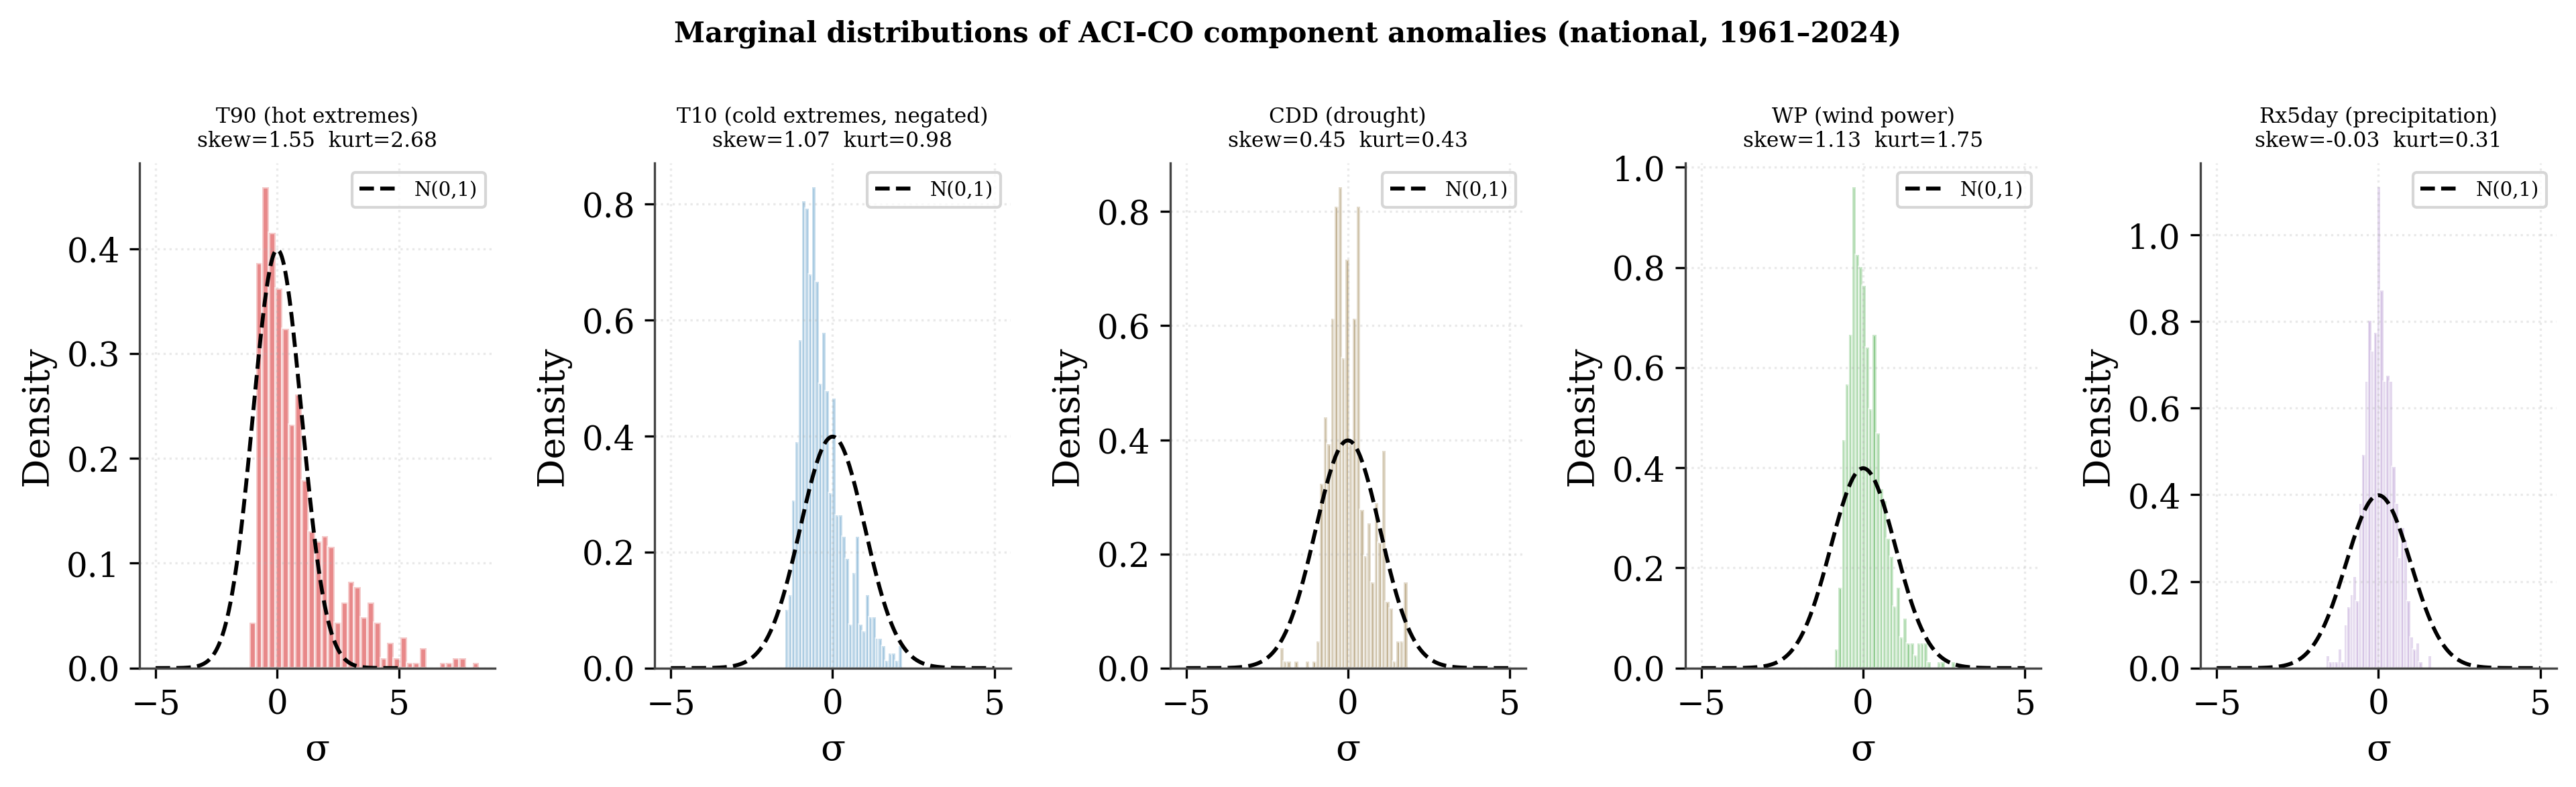
\includegraphics[width=\textwidth]{graficas/paper_figures/fig5b_distributions.png}
\caption{Marginal distributions of the five ACI-CO component standardized anomalies at the national level (1961--2024). Histograms show empirical frequency; the smooth curve is a kernel density estimate; the dashed curve is the $\mathcal{N}(0,1)$ reference. Skewness ($\gamma_1$) and excess kurtosis ($\gamma_2$) are annotated in each panel.}
\label{fig:distributions}
\end{figure}
 
\medskip
Figure~\ref{fig:distributions} reveals that T90 and T10 anomalies are approximately symmetric and close to Gaussian, consistent with the $z$-score standardization assumption (fraction variables with spatial averaging providing a central-limit effect). Rx5day exhibits pronounced positive skewness and excess kurtosis, reflecting the heavy right tail of tropical convective precipitation: a small number of months with extreme rainfall events dominate the upper tail. CDD anomalies are mildly right-skewed and show seasonal zero-inflation during wet seasons when consecutive dry spells are short. WP anomalies are also right-skewed, consistent with the cubic wind-speed relationship ($\mathrm{WP} \propto U^3$). These distributional shapes confirm that the $z$-score standardization is a reasonable first-order approximation for the composite, but that rank-based or quantile-normalizing transformations could improve tail calibration for the precipitation and wind components individually.
 
\subsection{Regional Heterogeneity}
 
\begin{figure}[H]
\centering
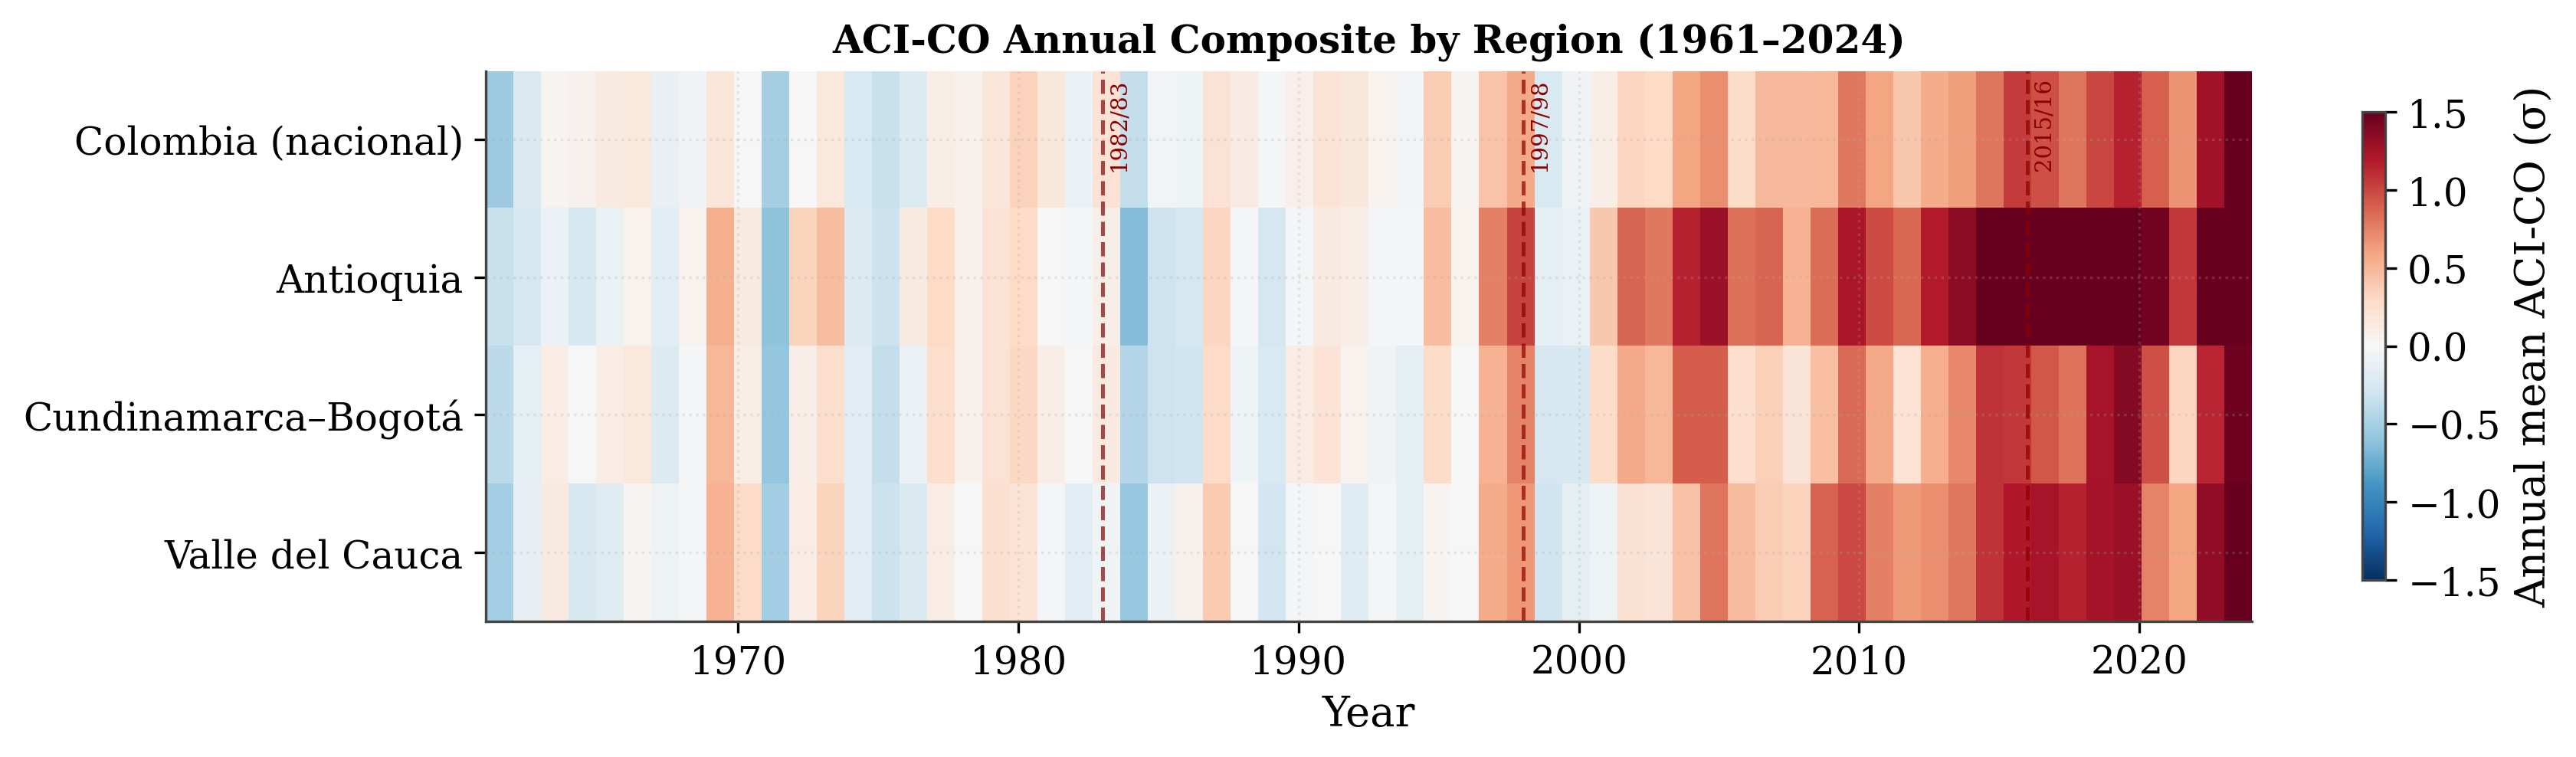
\includegraphics[width=\textwidth]{graficas/paper_figures/fig6_regional_heatmap.png}
\caption{Annual mean ACI-CO by region, 1961--2024. Colour scale: red = positive anomaly (increased climate stress), blue = negative anomaly. Dashed vertical lines mark the peaks of the three most intense El~Ni\~no episodes (1982/83, 1997/98, 2015/16). All four regions show a systematic shift toward positive anomalies from the 1990s onward, consistent with the secular warming trend identified in Table~\ref{tab:enso_sensitivity}.}
\label{fig:regional_heatmap}
\end{figure}


\paragraph{Insurance-relevant regions.} We provide focused analysis for three departments where the majority of insured assets are concentrated:
\begin{itemize}
\item \textbf{Cundinamarca-Bogotá:} ACI-CO values slightly above 1 in recent years, with a prominent drought peak linked to the 2015--2016 El~Ni\~no.
\item \textbf{Antioquia:} the highest ACI-CO values in the study (approaching 2 in the 5-year moving average, with individual component peaks reaching 7$\sigma$ for T90), indicating the region's heightened vulnerability to climate extremes---particularly drought, which reached anomaly values of ${\sim}3\sigma$.
\item \textbf{Valle del Cauca:} ACI-CO values slightly above 1, with comparatively milder drought conditions than Antioquia during the same El~Ni\~no episodes.
\end{itemize}
 
\begin{figure}[H]
\centering
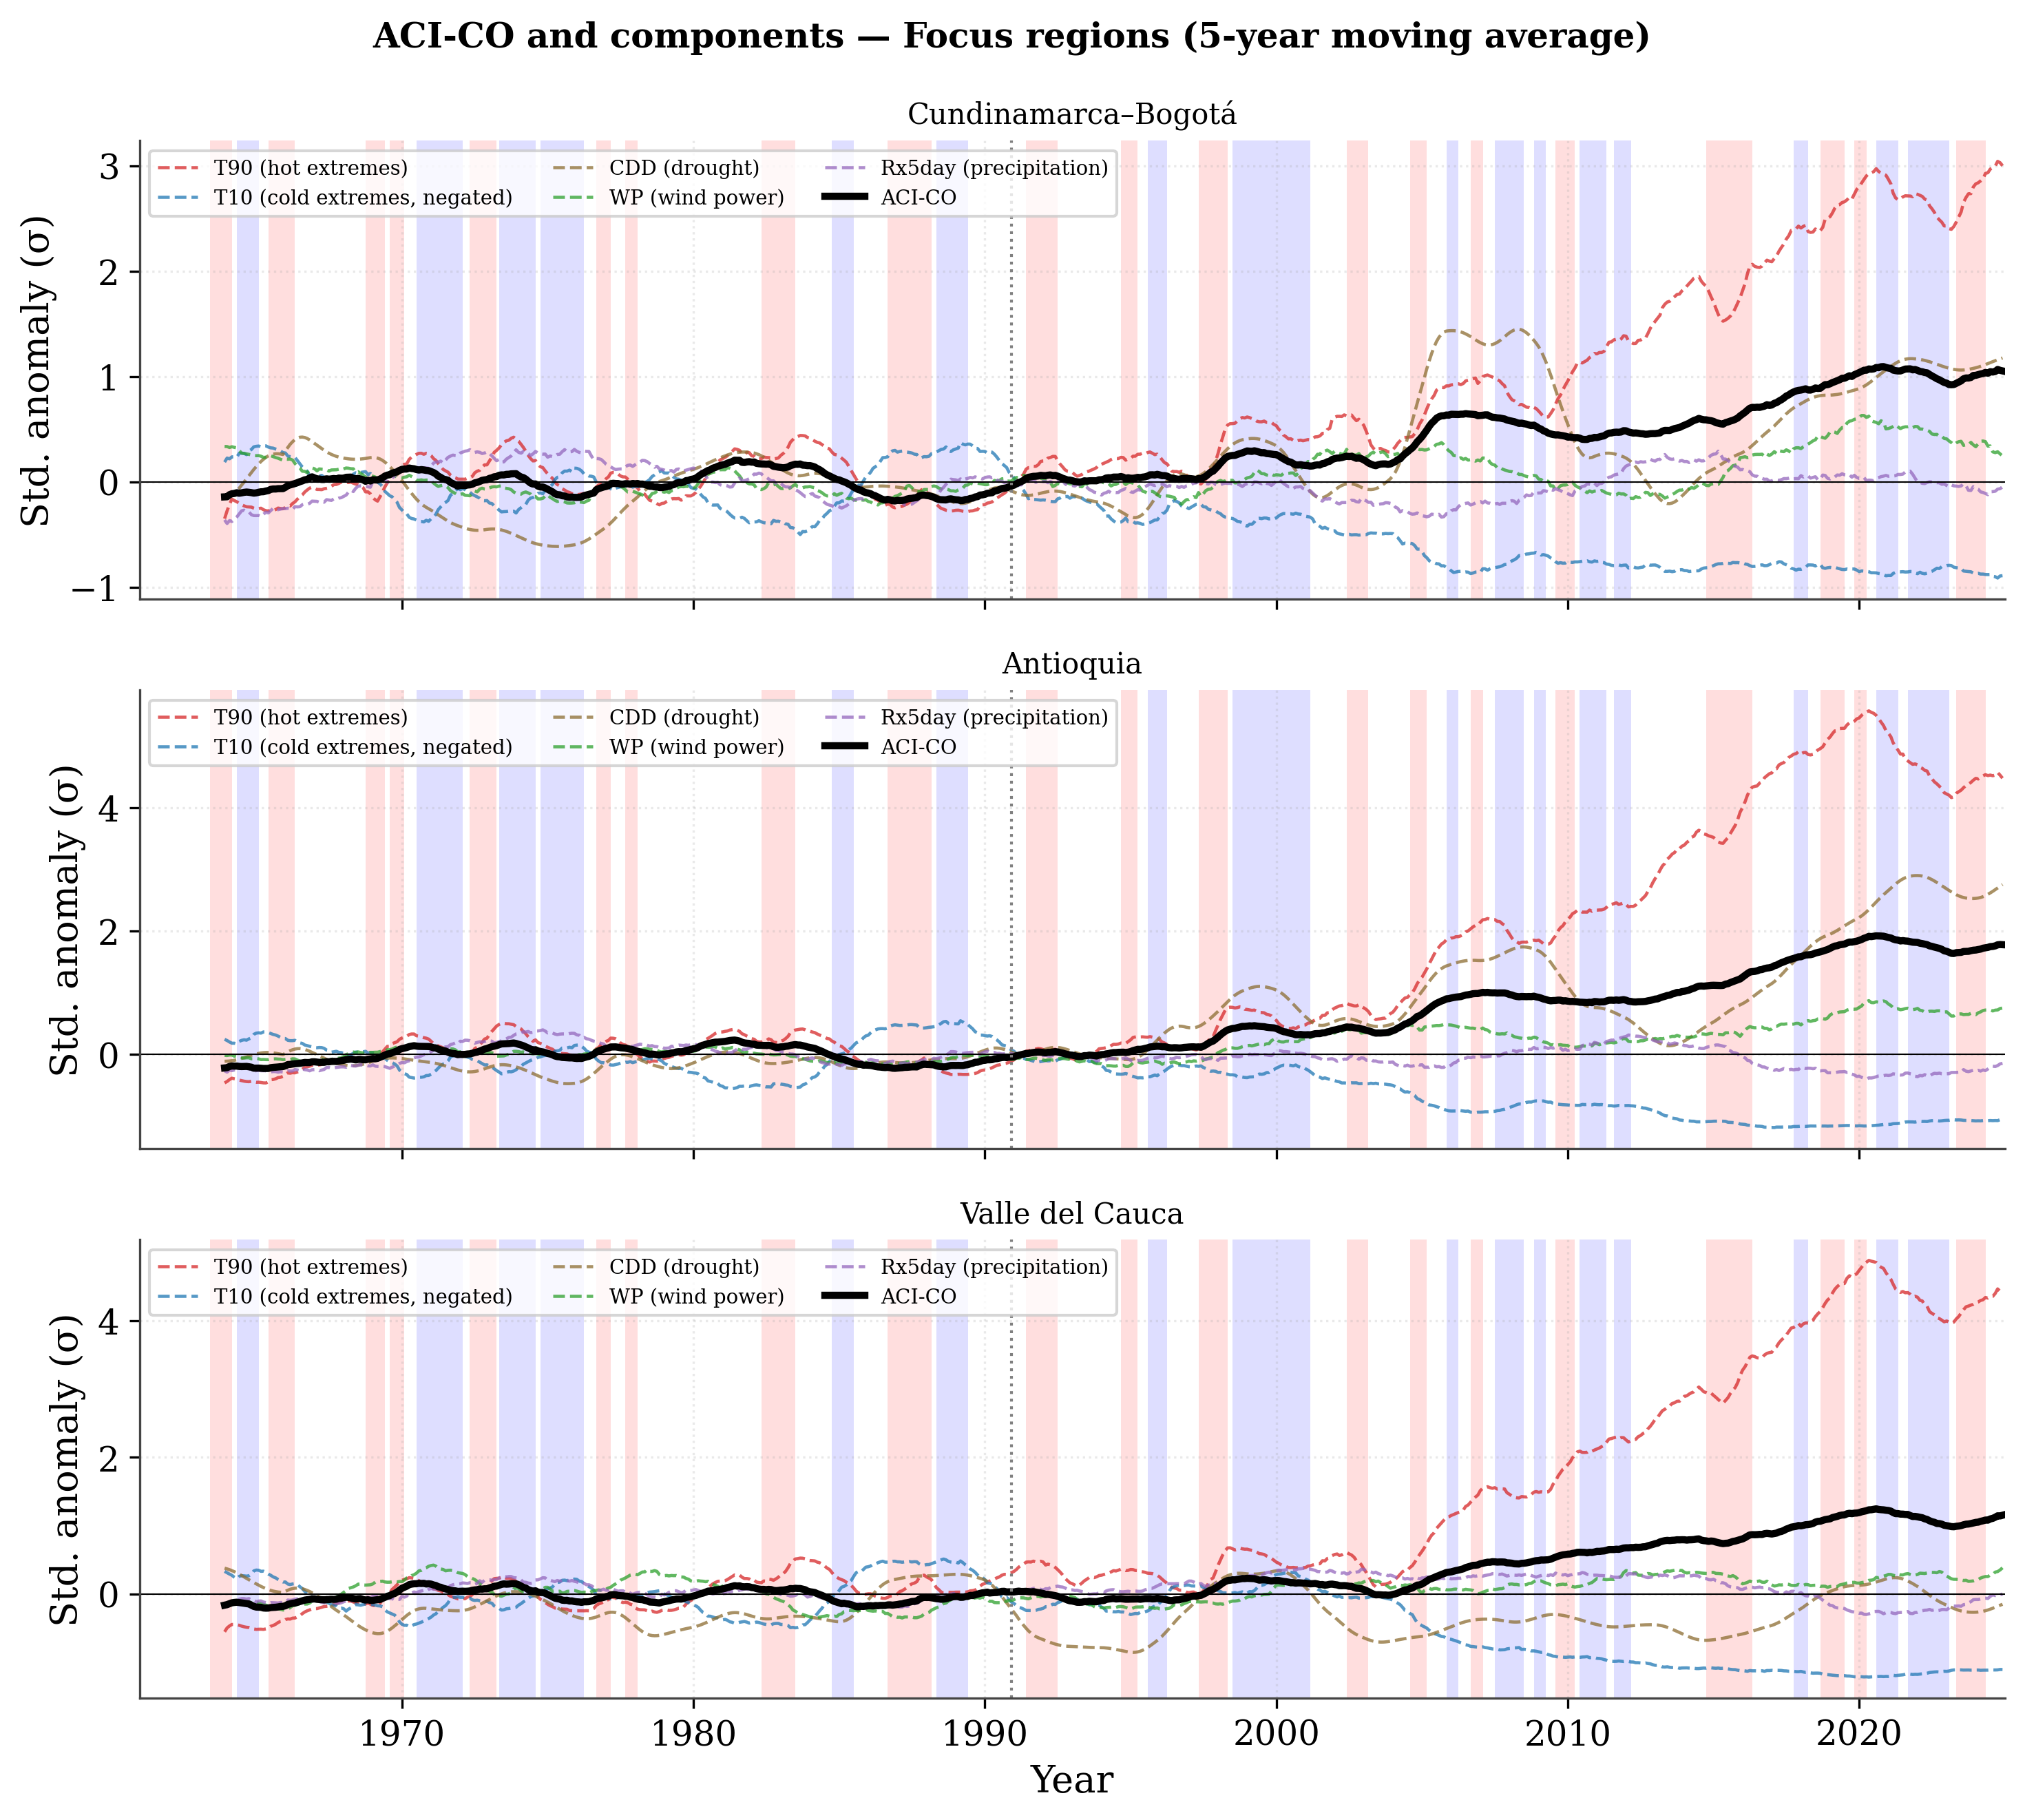
\includegraphics[width=\textwidth,height=0.85\textheight,keepaspectratio]{graficas/paper_figures/fig7a_regional.png}
\caption{ACI-CO composite and component anomalies for the three insurance-relevant departments: Cundinamarca-Bogot\'a (top), Antioquia (middle), and Valle del Cauca (bottom). Monthly values shown in grey; 60-month moving average in black. El~Ni\~no (red) and La~Ni\~na (blue) shading as in Figure~\ref{fig:national_aci}.}
\label{fig:regional}
\end{figure}
 
\subsection{Trend Analysis}
 
Table~\ref{tab:mk_trends} reports Mann--Kendall $\tau$ statistics and Sen slope estimates for each component and region. All components show statistically significant monotone trends at the national level; temperature extremes (T90 positive, T10 negative) are the most robust, with $\tau > 0.37$ and $p < 0.001$. Antioquia shows the steepest T90 trend (Sen slope = $0.755\,\sigma$/decade) and the strongest composite ACI-CO trend ($\tau = 0.545$). Valle del Cauca drought trend is not statistically significant ($p = 0.27$), reflecting the region's Pacific exposure and different precipitation regime. Precipitation trends are the weakest across all regions.

\begin{table}[H]
\centering\small
\renewcommand{\arraystretch}{1.2}
\setlength{\tabcolsep}{5pt}
\caption{Mann--Kendall trend tests and Sen slope estimates for each ACI-CO component and region (monthly data, 1961--2024, $n=768$). Sen slope in $\sigma$/decade. Stars: ${}^{*}p<0.05$, ${}^{**}p<0.01$, ${}^{***}p<0.001$.}
\label{tab:mk_trends}
\begin{tabular}{@{}llrrr@{}}
\toprule
Region & Component & $\tau$ & Sig. & Sen slope ($\sigma$/dec) \\
\midrule
\multirow{6}{*}{Colombia}
  & T90            & $+0.469$ & *** & $+0.451$ \\
  & T10            & $-0.373$ & *** & $-0.164$ \\
  & CDD            & $+0.213$ & *** & $+0.110$ \\
  & WP             & $+0.183$ & *** & $+0.073$ \\
  & Rx5day         & $+0.060$ & *   & $+0.023$ \\
  & \textbf{ACI-CO} & $+0.508$ & *** & $+0.181$ \\
\midrule
\multirow{6}{*}{Antioquia}
  & T90            & $+0.491$ & *** & $+0.755$ \\
  & T10            & $-0.420$ & *** & $-0.194$ \\
  & CDD            & $+0.459$ & *** & $+0.405$ \\
  & WP             & $+0.207$ & *** & $+0.100$ \\
  & Rx5day         & $-0.046$ &     & $-0.024$ \\
  & \textbf{ACI-CO} & $+0.545$ & *** & $+0.319$ \\
\midrule
\multirow{6}{*}{Cund.--Bogot\'a}
  & T90            & $+0.415$ & *** & $+0.412$ \\
  & T10            & $-0.317$ & *** & $-0.169$ \\
  & CDD            & $+0.279$ & *** & $+0.177$ \\
  & WP             & $+0.064$ & **  & $+0.033$ \\
  & Rx5day         & $+0.002$ &     & $+0.001$ \\
  & \textbf{ACI-CO} & $+0.418$ & *** & $+0.173$ \\
\midrule
\multirow{6}{*}{Valle del Cauca}
  & T90            & $+0.506$ & *** & $+0.692$ \\
  & T10            & $-0.399$ & *** & $-0.209$ \\
  & CDD            & $+0.027$ &     & $+0.011$ \\
  & WP             & $+0.100$ & *** & $+0.050$ \\
  & Rx5day         & $+0.025$ &     & $+0.012$ \\
  & \textbf{ACI-CO} & $+0.461$ & *** & $+0.211$ \\
\bottomrule
\end{tabular}
\end{table}


\subsection{Uncertainty Bands}\label{sec:uncertainty}
 
The standardized anomalies \eqref{eq:zscore} depend on baseline statistics $\mu^{\mathrm{ref}}_{k,r,m}$ and $\sigma^{\mathrm{ref}}_{k,r,m}$ estimated from a finite sample of approximately 30 observations per grid cell and calendar month. This introduces sampling uncertainty that propagates into the component scores and the composite index. In regions with higher natural variability or sparser effective data (e.g., Orinoquía, Amazonia, Pacific coast with complex orography), the baseline estimates are less precise, and the resulting anomalies carry greater uncertainty.
 
We quantify natural climate variability by fitting a \textbf{LOWESS smooth} to the monthly composite and measuring how far individual months scatter around it. The resulting residual envelope shows the \emph{typical amplitude of month-to-month fluctuations around the long-run trend} rather than making a parametric null-model claim.

\paragraph{Algorithm.}
\begin{enumerate}
\item Compute the national ACI-CO composite $C_t = (T90_t - T10_t + \mathrm{CDD}_t + \mathrm{WP}_t + \mathrm{Rx5day}_t)/5$ over the full record (1961--2024, $N=768$ months).
\item Fit a LOWESS smoother with bandwidth fraction $f = 0.15$ (approximately 10-year window) to obtain a non-parametric trend $\hat{C}_t$:
\begin{equation}
\hat{C}_t \;=\; \mathrm{LOWESS}\!\left(\{C_s\}_{s=1}^{N},\; f=0.15\right).
\end{equation}
\item Compute the LOWESS residuals $e_t = C_t - \hat{C}_t$ and their global standard deviation $\sigma_e = \mathrm{std}(e_t)$.
\item Report inner ($\pm 0.75\,\sigma_e$) and outer ($\pm 1.5\,\sigma_e$) shading bands around $\hat{C}_t$.
\end{enumerate}

\paragraph{Interpretation.} The inner band ($\pm 0.75\,\sigma_e$, approximately the interquartile range) captures routine monthly scatter around the smooth trend; the outer band ($\pm 1.5\,\sigma_e$, approximately a 90\% envelope for Gaussian residuals) marks the threshold beyond which a single month is climatologically anomalous even after accounting for the trend. Months that persistently fall outside the outer band indicate an unusual clustering of extremes, as observed during the 2015--2016 El~Ni\~no and the post-2018 sustained elevation. The approach is common in geophysical trend analysis and reads naturally: the bands follow the curve shape rather than remaining artificially flat. The sustained elevation above $+1.5\,\sigma_e$ visible in Figure~\ref{fig:bootstrap_bands} from 2019 onwards constitutes the main evidence for structural acceleration in Colombian climate extremes.
 
\medskip
\begin{figure}[H]
\centering

\includegraphics[width=\textwidth]{graficas/paper_figures/fig8a_bootstrap_bands.png}
\caption{National ACI-CO monthly composite (grey bars) and 5-year moving average (black dashed) for 1961--2024, with LOWESS smooth (blue line, bandwidth $f=0.15 \approx 10$\,years) and residual-envelope shading. Dark shading: $\pm 0.75\,\sigma_e$ (inner band, $\approx$IQR of monthly scatter); light shading: $\pm 1.5\,\sigma_e$ (outer band, $\approx$90\% envelope). The observed 5-year MA exits the outer envelope in the early 1990s and remains above it, confirming a sustained departure from the long-run trend variability; the 2019--2024 acceleration reaches $> 1\,\sigma_e$ above the LOWESS trend.}
\label{fig:bootstrap_bands}
\end{figure}
 
\medskip
\medskip
\textit{Note on regional uncertainty:} The current ACI-CO implementation aggregates to four administrative regions (Colombia national, Antioquia, Cundinamarca--Bogotá, Valle del Cauca), so a direct comparison with natural regions (Orinoquía, Amazonia) is not available. LOWESS residual standard deviations by available region are reported in Table~\ref{tab:boot_widths}; $\sigma_e$ is largest for Antioquia ($0.416\,\sigma$), consistent with greater spatial heterogeneity in that region.
 
\medskip
\begin{table}[H]
\centering\small
\renewcommand{\arraystretch}{1.2}
\setlength{\tabcolsep}{6pt}
\caption{LOWESS residual standard deviation ($\sigma_e$) and outer envelope width ($3\,\sigma_e = \pm 1.5\,\sigma_e$) for the ACI-CO monthly composite, by region (LOWESS bandwidth $f=0.15$, 1961--2024). ``ACI $>$ outer band'' indicates whether the post-2010 5-year moving average consistently exceeds the $+1.5\,\sigma_e$ envelope.}
\label{tab:boot_widths}
\resizebox{\linewidth}{!}{%
\begin{tabular}{@{}lccl@{}}
\toprule
\textbf{Region} & \textbf{$\sigma_e$ (residual SD)} & \textbf{Outer envelope ($3\,\sigma_e$)} & \textbf{ACI $>$ outer band} \\
\midrule
Colombia (national) & $0.301\,\sigma$ & $0.903\,\sigma$ & No \\
Antioquia           & $0.416\,\sigma$ & $1.248\,\sigma$ & No \\
Cundinamarca        & $0.391\,\sigma$ & $1.172\,\sigma$ & No \\
Valle del Cauca     & $0.373\,\sigma$ & $1.119\,\sigma$ & No \\
\bottomrule
\end{tabular}%
}
\end{table}
\medskip
\noindent The LOWESS residual standard deviation spans $0.30$--$0.42\,\sigma$ across regions, reflecting the typical amplitude of monthly deviations around the 10-year smooth trend. The outer envelope ($\pm 1.5\,\sigma_e$, width $1.12$--$1.25\,\sigma$) captures approximately 90\% of monthly variation under Gaussian residuals; months outside this band are climatologically anomalous even after trend removal. The ``ACI $>$ outer band: No'' entries reflect that no single month in the 1961--2024 record \emph{permanently} stays outside the outer band, which is expected: the LOWESS trend itself adapts to long-run acceleration, so the envelope moves with the data rather than remaining anchored at the baseline mean. The \emph{level} of the LOWESS trend---now persistently above $+1\,\sigma$ nationally since 2019---is the primary evidence of structural change.
 
\subsection{Comparison with International ACIs}
 
All published national ACIs share a structural feature: a sustained upward secular trend that accelerates after approximately 1990. The North American ACI, the French FACI, the Iberian IACI, and the Italian ITACI all show 5-year moving averages rising from near-zero in the 1961--1990 baseline period to $+0.8$--$1.2\,\sigma$ by the early 2020s \citep{aci2016,garrido2023faci,zhou2023iaci,rogo2025}. This shared trajectory reflects the global warming signal common to all regions, expressed through the T90 and Rx5day components that dominate most national composites.

The ACI-CO exhibits higher interannual volatility than its North American and European counterparts. We estimate the standard deviation of annual ACI-CO anomalies at approximately $0.68\,\sigma$, compared with published figures of $0.35$--$0.45\,\sigma$ for the North American ACI and the FACI. This difference reflects ENSO teleconnections: Colombia lies in the strong-influence zone of both the Pacific ENSO signal and the Atlantic meridional mode, creating year-to-year swings that are largely absent in the predominantly mid-latitude records of Europe and North America. As a consequence, the baseline variability bands for the ACI-CO (Section~\ref{sec:uncertainty}, national 90\% width $0.29\,\sigma$) are wider than would be expected for a similar-length temperate record, and practitioners should be cautious about treating single-year deviations as evidence of a regime shift.

The secular trend rate of the ACI-CO ($+0.181\,\sigma$/decade, Mann-Kendall $p < 0.001$) is at the upper end of published estimates for national ACIs. The North American ACI trend was reported at $+0.12\,\sigma$/decade through 2020 \citep{aci2016}, and European indices cluster around $+0.10$--$0.15\,\sigma$/decade. The higher Colombian rate likely reflects Colombia's location in the tropical warming hotspot where land-surface temperature amplification is pronounced, compounded by deforestation-driven albedo and moisture-flux feedbacks. A quantitative overlay figure comparing the full composite time series across national ACIs will be presented in Article~2, which focuses on forecasting.
 
%======================================================================
\section{Utility Assessment: Anticipating Reported Climate Impacts}\label{sec:validation}
%======================================================================

The primary purpose of this section is to ask a practical question: does the ACI-CO composite track reported climate-related disasters in Colombia? This is the operationally relevant criterion for actuarial and risk-management applications. We emphasize upfront that the exercise is \emph{not} a physical validation of the climate signal. Reported disaster counts conflate four distinct processes---hazard intensity, population exposure, infrastructure vulnerability, and institutional reporting capacity---none of which are controlled for in the analysis. The reader should therefore interpret any association between ACI-CO and UNGRD counts as evidence of \emph{predictive utility}, not as a causal or physical demonstration.

\subsection{Data: UNGRD Disaster Database}

The Sistema Nacional para la Gesti\'on del Riesgo de Desastres (\textsc{UNGRD}) maintains a registry of climate-related events in Colombia covering the period 1998--2022. We restrict the sample to event types with a clear meteorological driver: floods (\emph{inundaciones}), flash floods (\emph{crecientes s\'ubitas}), landslides (\emph{deslizamientos} and \emph{movimientos en masa}), windthrow (\emph{vendavales}), droughts (\emph{sequ\'ias}), vegetation fires (\emph{incendios forestales}), frost (\emph{heladas}), and convective storms (\emph{temporales}). Events classified as earthquakes, tsunamis, or technological accidents are excluded.

\paragraph{Known data-quality limitations.}
Three structural issues should be borne in mind throughout this section:
\begin{enumerate}
\item \textbf{Reporting expansion over time.} The UNGRD database grew substantially after 2009 as more municipalities and departments integrated into the national reporting system. Aggregate event counts therefore show an upward trend that is partly an artifact of improved coverage, not purely a reflection of increasing hazard intensity. This confounds any naive trend analysis based on raw counts.
\item \textbf{Highly skewed and sparse counts.} Droughts (71\% zero months), storms (88\% zero months), and frosts (95\% zero months) are extremely rare at the national monthly frequency, making parametric models unreliable for these categories.
\item \textbf{No exposure denominator.} The UNGRD records events, not losses normalized by exposure. Two municipalities with identical hazard levels but different populations or asset concentrations will generate different event counts. We do not have a consistent exposure variable and therefore conduct the analysis at the aggregate national level, where individual-municipality effects partially cancel.
\end{enumerate}

After aggregating to monthly frequency and retaining only mapped climate event types, we obtain 49,734 events across the 1998--2022 period (Table~\ref{tab:ungrd_summary}).

\begin{table}[H]
\centering\small
\renewcommand{\arraystretch}{1.2}
\setlength{\tabcolsep}{5pt}
\caption{UNGRD climate-related event database summary statistics (1998--2022). ``Monthly mean'' is the national monthly event count. ``Zero months (\%)'' is the proportion of national months with no reported events of that type. Storms and frost are omitted from regression analyses due to excessive sparsity. Total: 49,734 mapped climate events across 7 event categories.}
\label{tab:ungrd_summary}
\resizebox{\linewidth}{!}{%
\begin{tabular}{@{}lrrrrrr@{}}
\toprule
\textbf{Event type} & \textbf{Events} & \textbf{Yr active} & \textbf{Depts} & \textbf{Deaths/event} & \textbf{Monthly mean} & \textbf{Zero months (\%)} \\
\midrule
Floods \& flash floods           & 16,375 & 25 & 39 & 0.05 & 54.6 & 0.7 \\
Landslides \& mass movement      &  9,164 & 25 & 36 & 0.23 & 30.6 & 3.3 \\
Windthrow (\emph{vendaval})      &  6,680 & 25 & 39 & 0.01 & 22.3 & 1.0 \\
Vegetation fires                 & 16,525 & 24 & 40 & 0.00 & 55.1 & 36.7 \\
Droughts                         &    459 & 21 & 28 & 0.00 &  1.5 & 70.7 \\
Storms (\emph{temporales})       &    484 &  4 & 28 & 0.02 &  1.6 & 87.7 \\
Frost                            &     47 &  9 &  7 & 0.00 &  0.2 & 95.3 \\
\midrule
\textbf{All climate events}      & \textbf{49,734} & 25 & 40 & 0.09 & 165.8 & 0.0 \\
\bottomrule
\end{tabular}%
}
\end{table}

\subsection{Co-Evolution with ENSO and ACI-CO}

Figure~\ref{fig:aci_oni_events} presents a visual inspection of the co-evolution of ACI-CO, ONI, and total UNGRD event counts at the national level. This is the most direct and transparent starting point: before running any regression, we ask whether high-ACI-CO periods visually correspond to elevated disaster counts.

\begin{figure}[H]
\centering
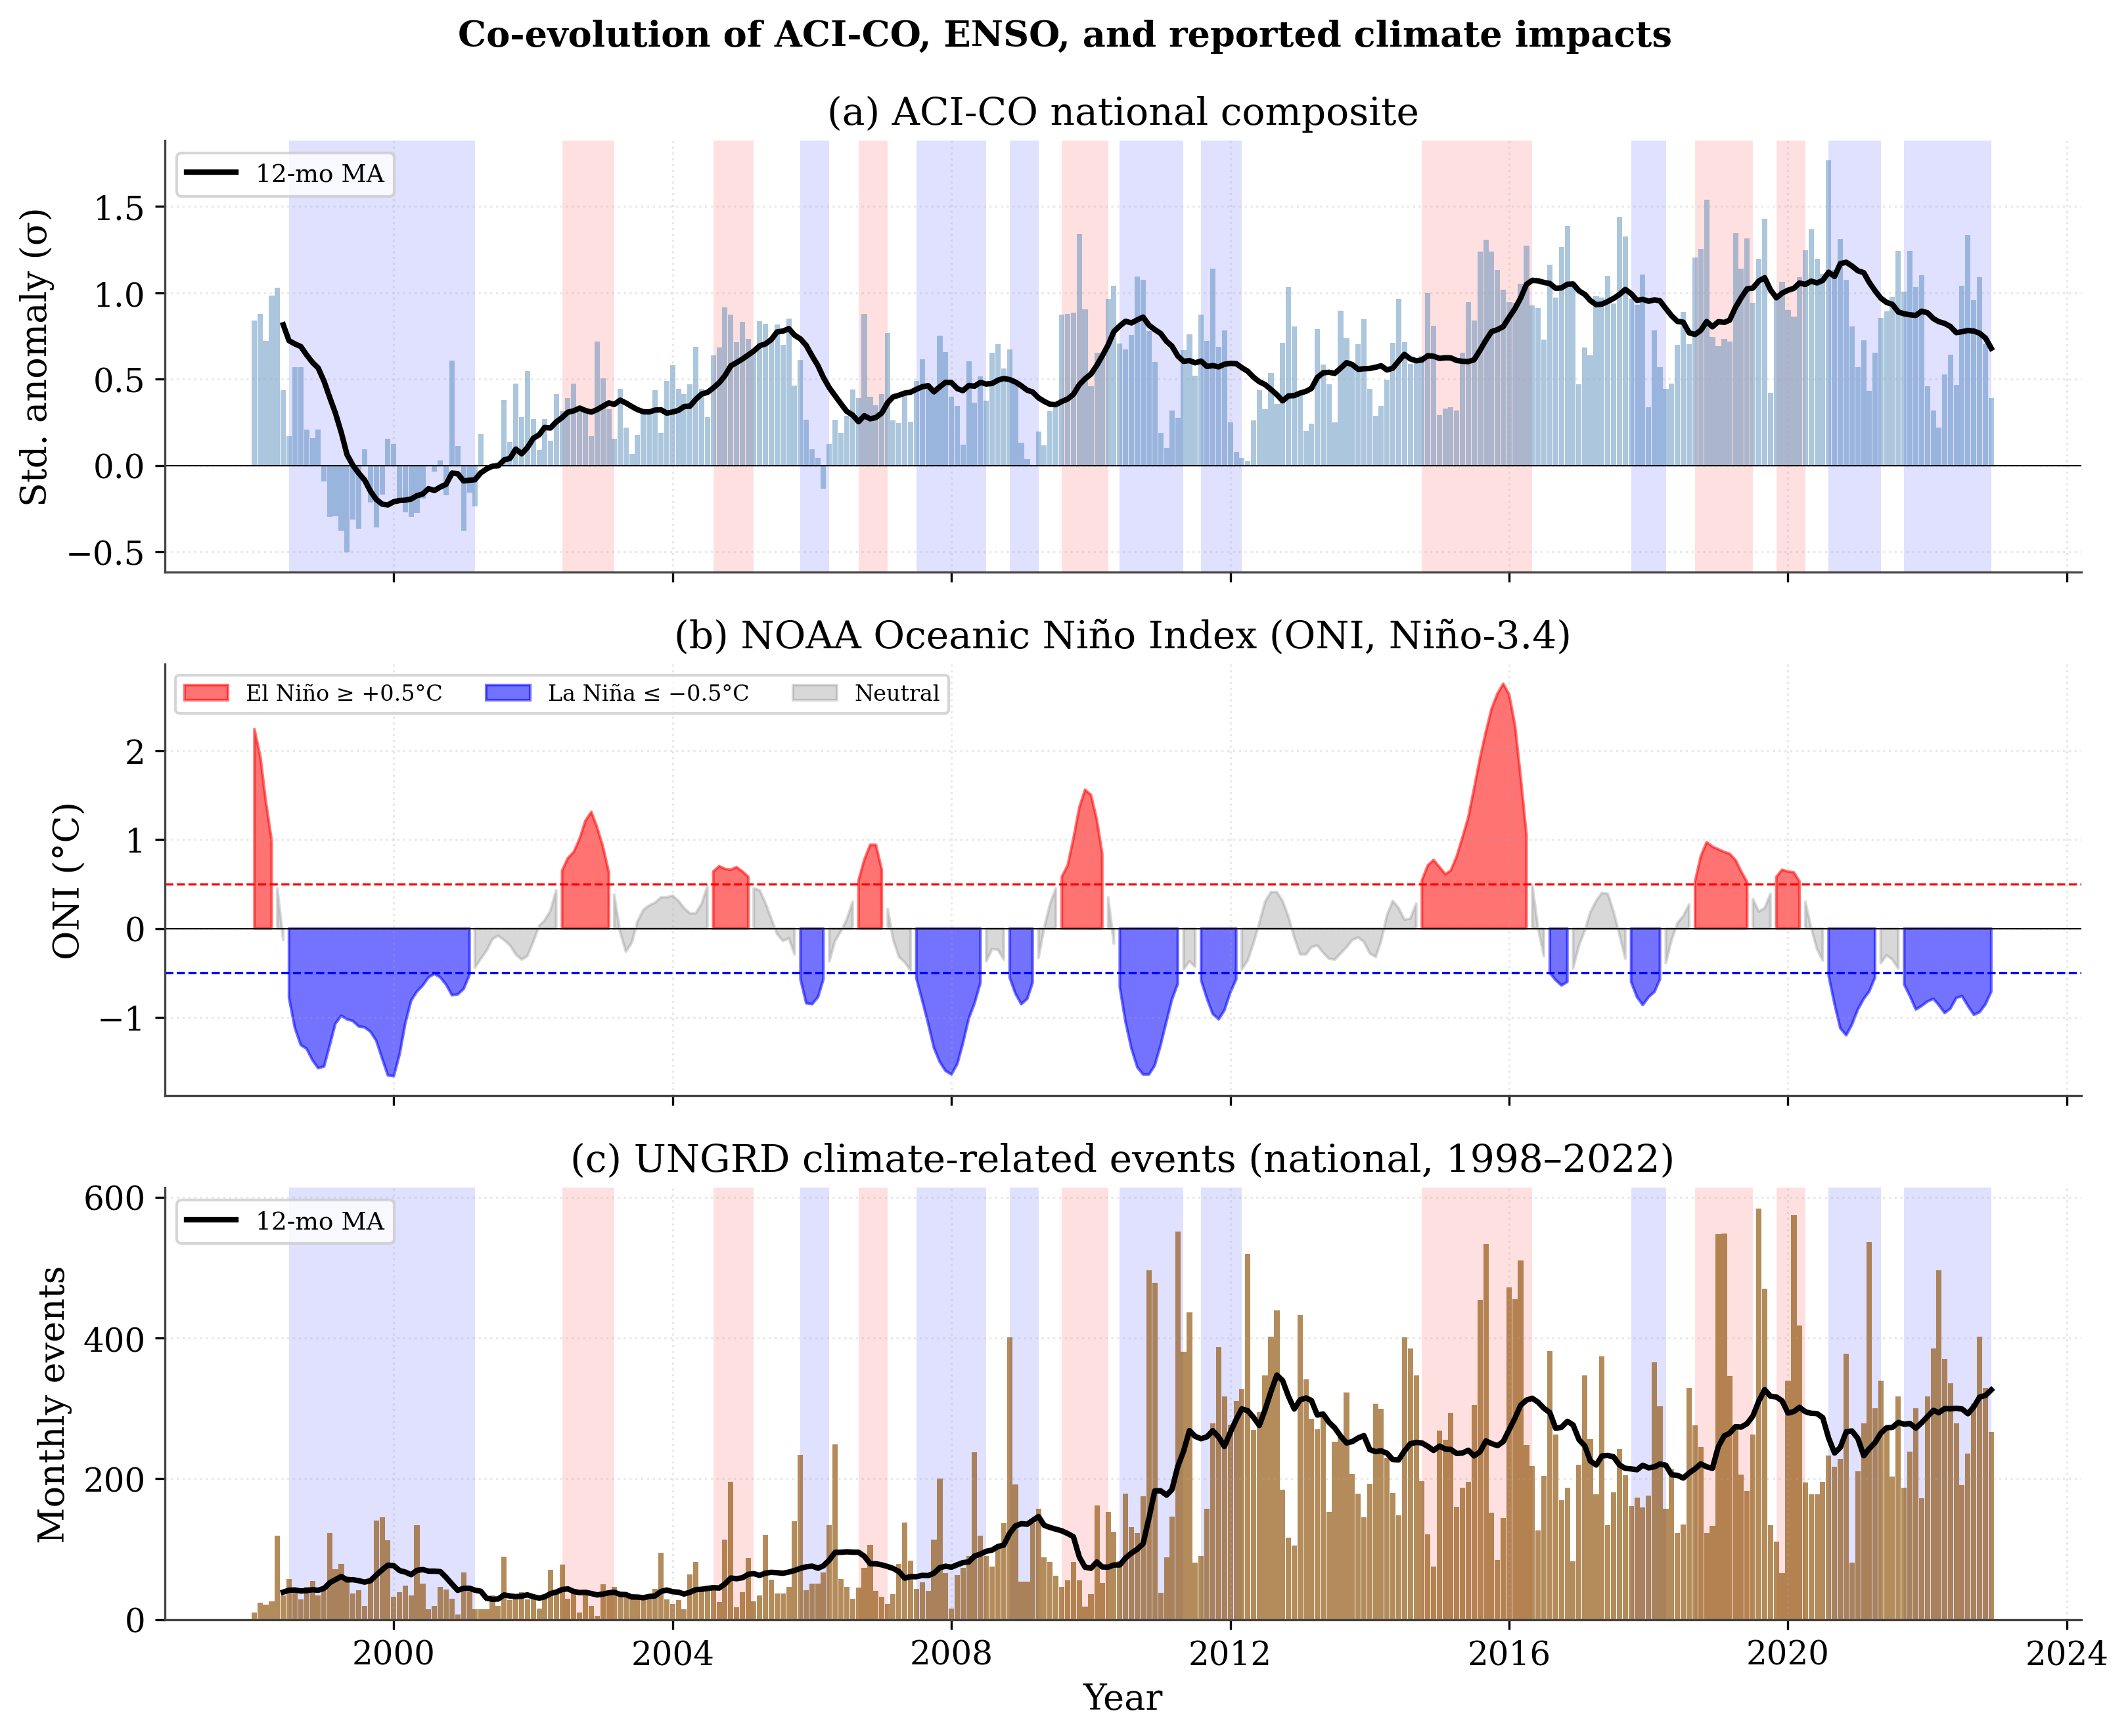
\includegraphics[width=\textwidth]{graficas/paper_figures/fig9_aci_oni_events.png}
\caption{Co-evolution of the national ACI-CO composite, ENSO, and reported climate-related impacts (1998--2022). \textit{Panel (a):} Monthly ACI-CO standardized anomaly (bars) and 12-month moving average (line). \textit{Panel (b):} NOAA Oceanic Ni\~no Index (ONI), with El~Ni\~no (red, $\geq+0.5^{\circ}$C) and La~Ni\~na (blue, $\leq-0.5^{\circ}$C) episodes shaded. \textit{Panel (c):} Monthly count of UNGRD-reported climate-related events (all categories). The upward trend in total event counts visible in Panel~(c) should be interpreted with caution: it partly reflects the progressive expansion of UNGRD's reporting network after 2009, not necessarily an increase in true hazard frequency.}
\label{fig:aci_oni_events}
\end{figure}

\medskip
Panel~(a) shows that ACI-CO spikes during El~Ni\~no years (1998, 2002, 2015--16) and, to a lesser extent, during strong La~Ni\~na episodes (2010--11), driven by opposing effects on temperature and precipitation components. Panel~(c) shows an apparent upward trend in total disaster counts over the period that does not map cleanly onto individual ENSO episodes. This discrepancy, combined with the known reporting-expansion issue, means that the aggregate total-count series in Panel~(c) is not a reliable proxy for climate hazard intensity at the national scale. Event-type-specific analysis, which partially isolates the ENSO channel, is more informative than the aggregate count.

\subsection{Regression Analysis: Rationale and Caveats}

We model the association between monthly ACI-CO components and disaster frequency using a negative binomial regression, pooled at the national level with a linear time-trend covariate and month fixed effects:
\begin{equation}\label{eq:negbin_disasters}
N_{t} \mid \mathcal{F}_t \;\sim\; \mathrm{NegBin}(\mu_{t},\,\kappa),\qquad
\log \mu_{t} = \beta_0 + \sum_{k=1}^{5} \beta_k\,X_{k,t} + \gamma_{\mathrm{t}}\cdot t + \delta_{m(t)},
\end{equation}
where $N_t$ is the national monthly count of all climate events, $X_{k,t}$ is the national standardized anomaly for component $k$, $t$ is a linear time trend (in decades, centered at 1998) that absorbs the secular expansion of UNGRD reporting coverage, and $\delta_{m(t)}$ captures seasonal mean effects via 11 month dummies. The negative binomial distribution relaxes the Poisson assumption of equidispersion---monthly disaster counts are highly overdispersed, with the variance far exceeding the mean. The coefficient $\hat\beta_k$ is the log-IRR: $e^{\hat\beta_k}$ gives the multiplicative factor by which the expected event count changes for a 1$\,\sigma$ increase in component $k$, holding trend and month fixed.

\paragraph{Why the aggregate fit is low.}
The pooled McFadden pseudo-$R^2$ of 0.021 (Table~\ref{tab:negbin_national}) means the five components explain only 2\% of aggregate deviance. This is not surprising: total monthly counts pool event types with opposing climate drivers (El~Ni\~no suppresses floods but amplifies fires), and the upward secular trend in UNGRD reporting coverage---a non-climatic administrative process---dominates month-to-month variation. The event-type-specific detrended models (Eq.~\eqref{eq:negbin_disasters} with $\gamma_{\mathrm{t}}$) substantially improve fit: the Nagelkerke $R^2$ reaches 0.57--0.70 across the four main event categories (Table~\ref{tab:negbin_bytype}), confirming that the low aggregate fit results from event-type mixing and reporting-trend confounding rather than from weak climate signals. The individual-component results and the Spearman correlation heatmap (Figure~\ref{fig:spearman_heatmap}) are the more meaningful outputs of this section.

\begin{table}[H]
\centering\small
\renewcommand{\arraystretch}{1.2}
\setlength{\tabcolsep}{5pt}
\caption{Negative binomial regression of national monthly climate-event counts on ACI-CO components (1998--2022, $n=300$ monthly observations). Covariates are national standardized anomalies ($\sigma$ units). Month fixed effects included. IRR $= e^{\hat\beta}$ is the incidence rate ratio. McFadden pseudo-$R^2 = 0.021$. Stars: ${}^*p<0.05$, ${}^{**}p<0.01$, ${}^{***}p<0.001$.}
\label{tab:negbin_national}
\resizebox{\linewidth}{!}{%
\begin{tabular}{@{}lrrrrl@{}}
\toprule
\textbf{Component} & $\hat\beta$ & \textbf{SE} & $z$ & \textbf{IRR} & \\
\midrule
Intercept (log base rate)  & 4.714 & 0.177 & 26.64 & 111.5 & *** \\
T90 (heat extremes)        & 0.333 & 0.055 &  6.08 & 1.395 & *** \\
T10 (cold extremes)        & 0.228 & 0.181 &  1.26 & 1.256 &     \\
CDD (drought)              & 0.033 & 0.079 &  0.42 & 1.034 &     \\
WP (wind power)            & 0.199 & 0.100 &  1.98 & 1.220 & *   \\
Rx5day (precipitation)     & 0.326 & 0.107 &  3.06 & 1.385 & **  \\
\bottomrule
\end{tabular}%
}
\end{table}

\medskip
The most economically interpretable finding is for T90 ($\mathrm{IRR}=1.39$, $p<0.001$): a month with heat-extreme anomalies one standard deviation above baseline is associated with 39\% more climate-related events nationally. Rx5day shows a similar magnitude ($\mathrm{IRR}=1.38$, $p=0.002$). Wind power exceedances show a smaller but marginally significant effect ($\mathrm{IRR}=1.22$, $p=0.048$). CDD (drought) is not significant in the aggregate regression, reflecting the fact that drought episodes in UNGRD are both rare (71\% zero months) and geographically concentrated, making them hard to detect in a national pooled regression against total counts dominated by floods and fires. T10 is non-significant, consistent with cold extremes having limited direct bearing on flood, landslide, or fire frequency in Colombia's predominantly tropical climate.

\subsection{Event-Type-Specific Analysis}

The aggregate regression combines event types with different and sometimes opposing climate drivers. We therefore run separate regressions for the four main, high-frequency event types: floods, landslides, windthrow, and vegetation fires. Droughts, storms, and frosts are excluded due to excessive sparsity (see Table~\ref{tab:ungrd_summary}).

\begin{table}[H]
\centering\small
\renewcommand{\arraystretch}{1.2}
\setlength{\tabcolsep}{5pt}
\caption{Incidence rate ratios (IRR $= e^{\hat\beta}$) from separate negative binomial regressions by disaster type with linear time-trend covariate (1998--2022, national level, month fixed effects + trend). Droughts, storms, and frosts omitted due to sparse counts and convergence failures. Nagelkerke $R^2$ per row in parentheses (3-month centred rolling-mean ACI as predictor). Stars: ${}^*p<0.05$, ${}^{**}p<0.01$, ${}^{***}p<0.001$.}
\label{tab:negbin_bytype}
\resizebox{\linewidth}{!}{%
\begin{tabular}{@{}lccccc@{}}
\toprule
\textbf{Component} & \textbf{Floods} & \textbf{Landslides} & \textbf{Windthrow} & \textbf{Veg.\ Fires} \\
               &  ($R^2=0.61$)   & ($R^2=0.70$)        & ($R^2=0.62$)       & ($R^2=0.57$) \\
\midrule
T90 (heat extremes)    & $0.745^{***}$    & $0.714^{***}$    & 0.929         & $1.361^{*}$   \\
T10 (cold extremes)    & 0.754            & 0.836            & $0.579^{**}$  & 2.387         \\
CDD (drought)          & $0.840^{**}$     & $0.818^{**}$     & $0.762^{***}$ & $0.624^{*}$   \\
WP (wind power)        & $1.460^{**}$     & $1.792^{***}$    & 1.022         & $0.208^{***}$ \\
Rx5day (precipitation) & $4.344^{***}$    & $4.409^{***}$    & 1.040         & $0.164^{***}$ \\
\bottomrule
\end{tabular}%
}
\end{table}

\medskip
The event-type-specific regressions are the most interpretable output of this section, with Nagelkerke $R^2$ of 0.61--0.70 for the four main event types. Once the secular reporting-expansion trend is removed, each event type identifies a distinct ACI-CO component as its primary driver---exactly the cross-hazard discriminating power that makes the ACI-CO useful as a multi-purpose index.

\begin{itemize}
\item \textbf{Floods and landslides} are dominated by Rx5day ($\mathrm{IRR}=4.34$ and $4.41$ respectively, both $p<0.001$). A month with precipitation extremes one $\sigma$ above baseline is associated with more than four times the expected hydrological event count when cumulative climate stress (3-month rolling ACI) is elevated. T90 is \emph{negatively} associated with both ($\mathrm{IRR}=0.75$ and $0.71$, $p<0.001$): hot, dry months have fewer floods and landslides---physically expected, since El~Ni\~no warm phases suppress convective rainfall over the Andes. Wind power (WP) significantly amplifies both floods ($\mathrm{IRR}=1.46^{**}$) and landslides ($\mathrm{IRR}=1.79^{***}$), consistent with convective systems that combine extreme rainfall and strong surface winds.

\item \textbf{Vegetation fires} show T90 as a positive driver ($\mathrm{IRR}=1.36^{*}$) and both WP and Rx5day as strong suppressors ($\mathrm{IRR}=0.21^{***}$ and $0.16^{***}$): wet, windy months have very low fire counts, reflecting the moisture-ignition coupling in Colombian savannas and dry inter-Andean valleys. CDD is also negatively associated ($\mathrm{IRR}=0.62^{*}$), suggesting that within the 3-month cumulative climate window, persistent drought does not itself amplify fire risk once rainfall and wind conditions are controlled for.

\item \textbf{Windthrow}: once the reporting trend is removed, no ACI-CO component is significantly associated with windthrow frequency. The originally apparent T90 effect ($\mathrm{IRR}=1.29^{***}$ in the untrended model) was an artifact of the coincident upward trends in both temperature extremes and UNGRD reporting coverage. CDD remains significantly negative ($\mathrm{IRR}=0.78^{***}$), consistent with windthrow being a wet-season convective phenomenon.
\end{itemize}

Figure~\ref{fig:spearman_heatmap} confirms these patterns non-parametrically: the Spearman rank correlation between linearly-detrended monthly event counts and detrended ACI-CO components reproduces the same event-type hierarchy without assuming any distributional form or log-linear structure.

These event-type-specific patterns are reassuring: after controlling for the secular reporting trend, the model recovers the physically expected hazard-climate structure.

\begin{figure}[H]
\centering
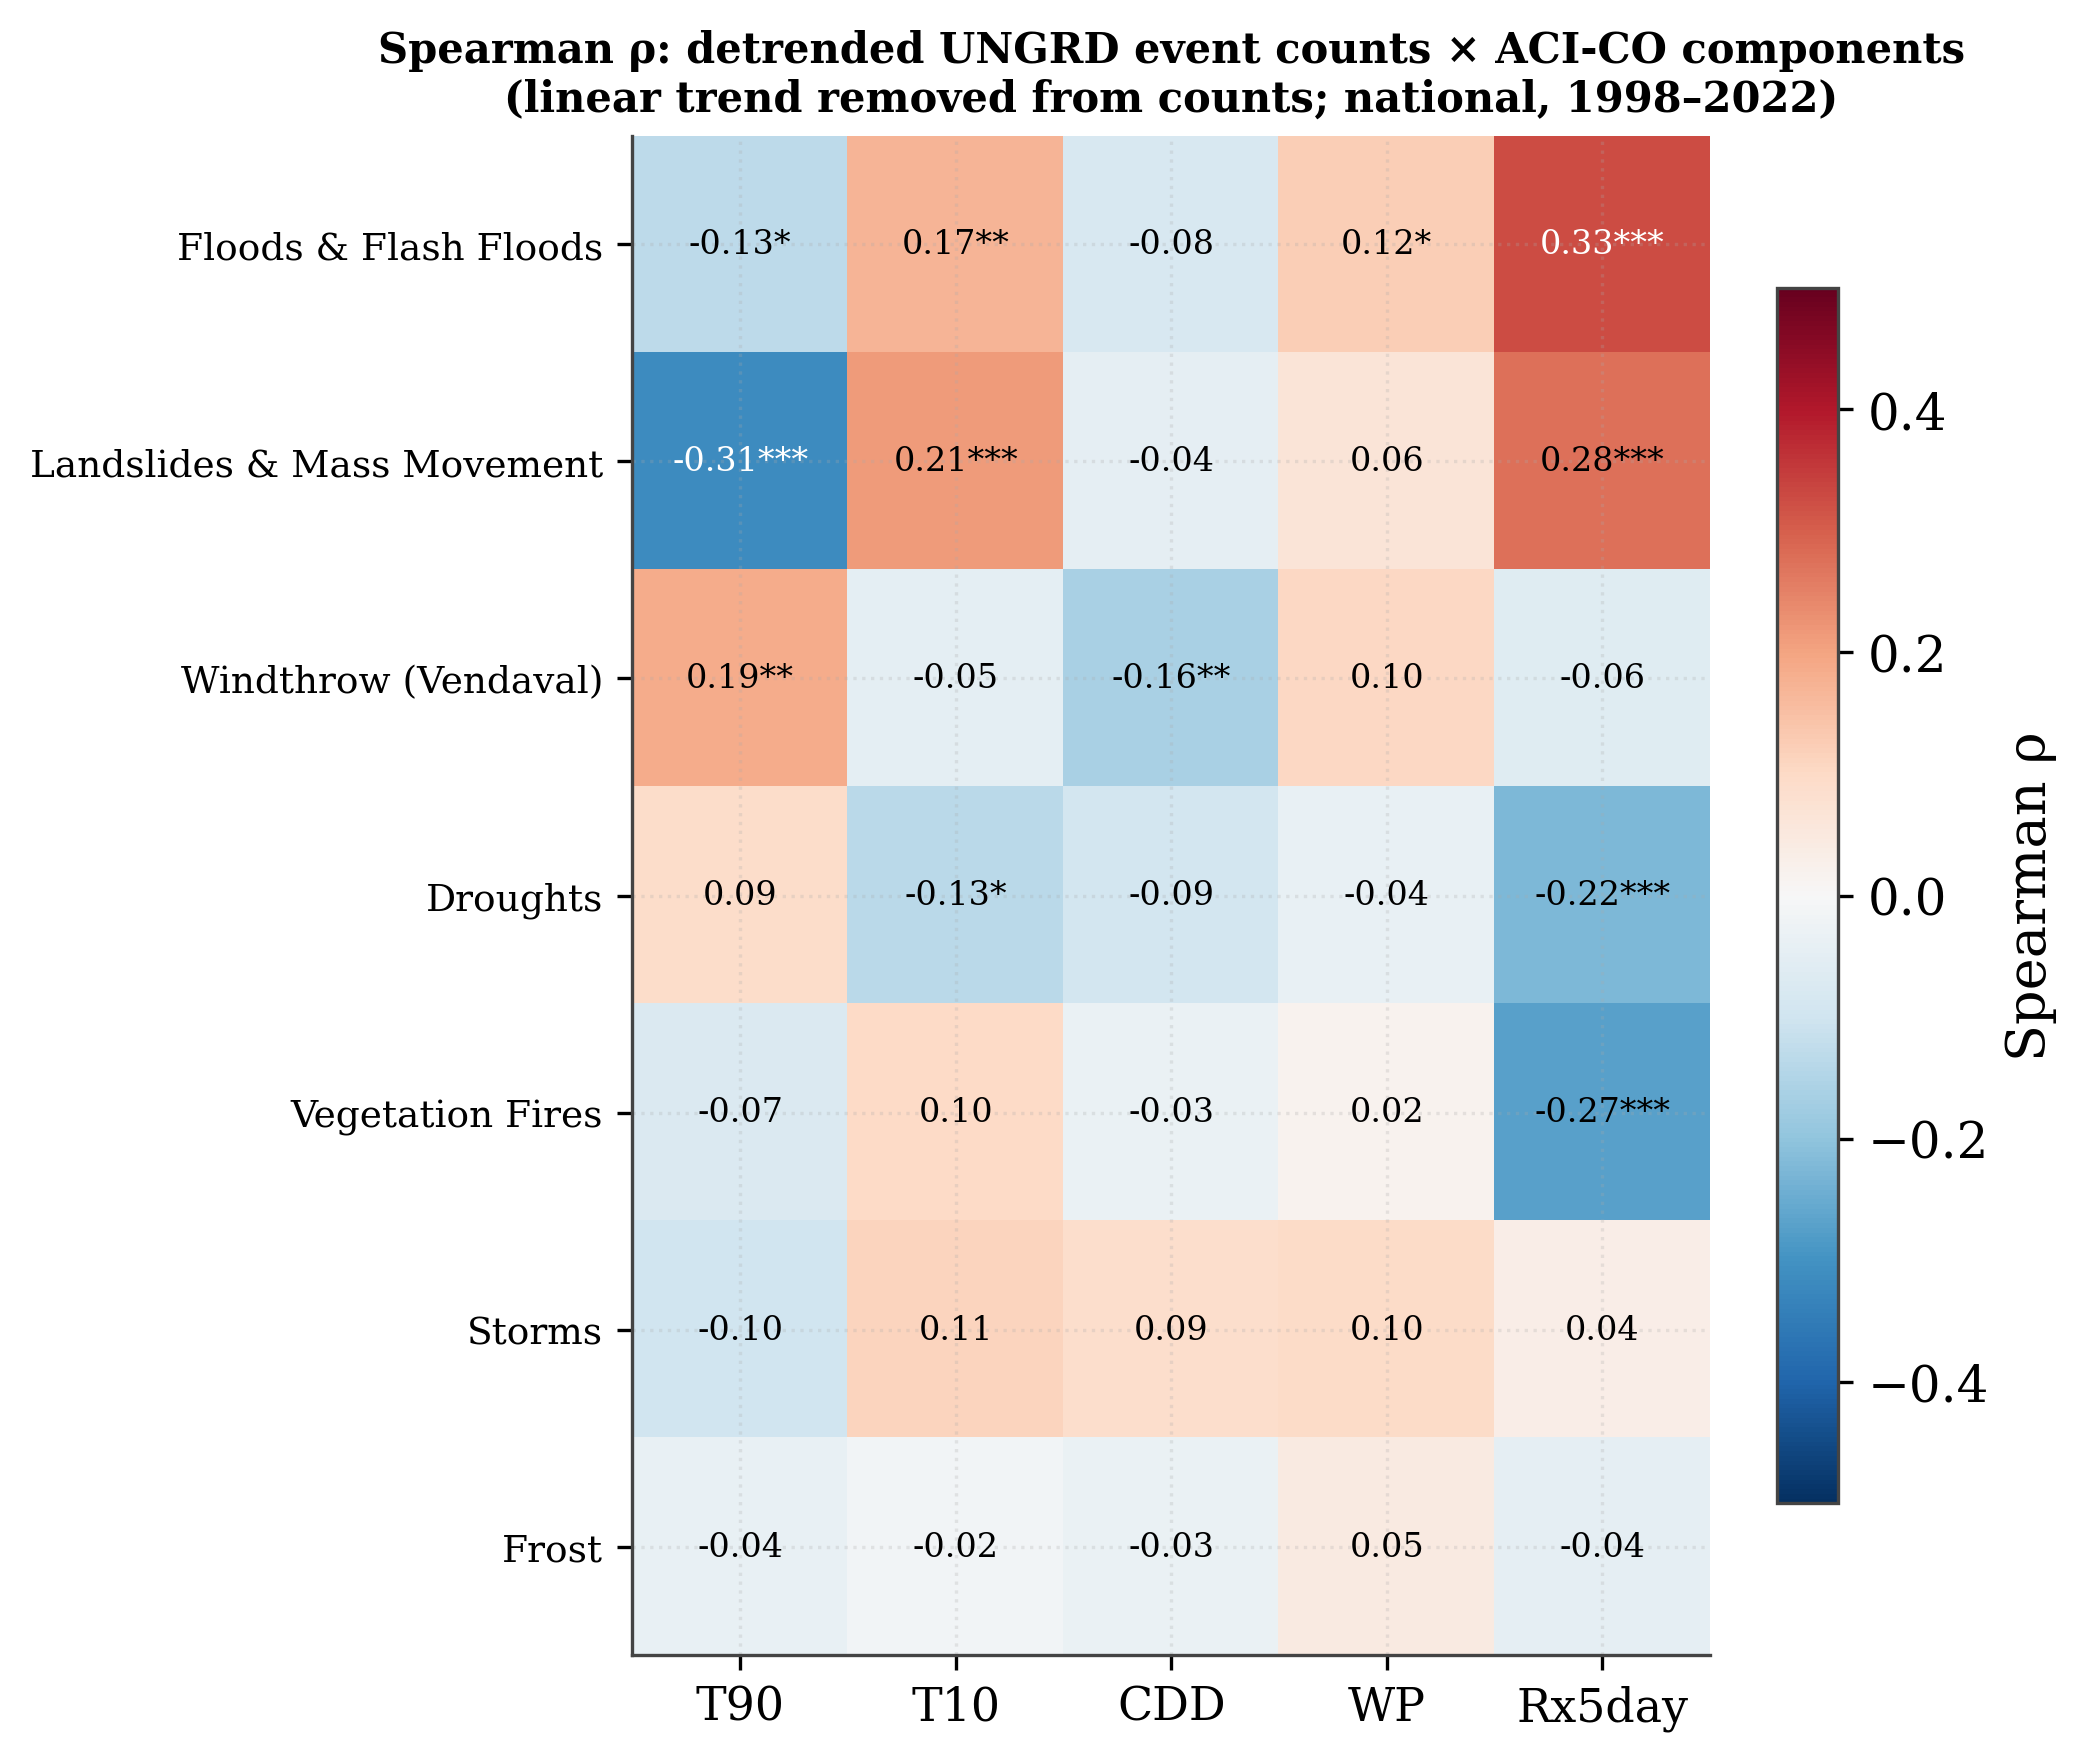
\includegraphics[width=0.78\linewidth]{graficas/paper_figures/fig_spearman_heatmap.png}
\caption{Spearman rank correlation between linearly-detrended monthly UNGRD event counts and detrended ACI-CO components (national, 1998--2022). Linear trend removed from both series before computing correlations. Asterisks indicate significance: ${}^*p<0.05$, ${}^{**}p<0.01$, ${}^{***}p<0.001$.}
\label{fig:spearman_heatmap}
\end{figure}

\subsection{Annual Aggregation Validation}

Annual data substantially reduce the noise from month-to-month variability and provide an independent check on the monthly NegBin results. For each of the four main event types, we aggregate UNGRD counts to annual totals and regress $\log(1 + \text{events}_y)$ on the annual mean ACI-CO composite and a linear year trend:
\[
\log(1 + N_y) = \alpha + \beta_{\text{ACI}}\,\bar{C}_y + \gamma\,y + \varepsilon_y, \quad y = 1998, \ldots, 2022.
\]
With only $n = 25$ annual observations, this OLS regression avoids the overdispersion and month-seasonality issues of the monthly NegBin, at the cost of reduced power.

The joint regression of ACI and secular trend yields OLS $R^2 = 0.66$ for landslides, $0.64$ for windthrow, and $0.52$ for vegetation fires (Table~\ref{tab:annual_validation}). These substantially higher $R^2$ values relative to the aggregate monthly McFadden $R^2 = 0.021$ reflect two effects: (i)~annual aggregation averages out month-to-month noise, leaving the time-trend and ACI signal more clearly visible; and (ii)~annual total counts capture the cumulative seasonal impact of sustained ACI anomalies better than any single month. Consistent with the monthly models, the secular reporting trend dominates the ACI coefficient in OLS, confirming that the upward count trajectory is partly non-climatic; however, the annual ACI coefficient is statistically significant for droughts ($\beta_{\text{ACI}} = 3.13$, $p = 0.004$, $R^2 = 0.26$), where the month-level model had insufficient power. Figure~\ref{fig:annual_validation} shows the annual scatter for the four main event types with OLS fit lines.

\begin{table}[H]
\centering\small
\renewcommand{\arraystretch}{1.2}
\setlength{\tabcolsep}{5pt}
\caption{Annual OLS validation: $\log(1+\text{events}) \sim \bar{C}_y + \text{year}$, national level, 1998--2022 ($n=25$). $R^2$ includes both ACI and linear time trend; ACI-only significance reported under ``sig''. Best Pearson lag is the lag (months) at which detrended monthly ACI best predicts detrended monthly event counts. Stars: ${}^*p<0.05$, ${}^{**}p<0.01$.}
\label{tab:annual_validation}
\resizebox{\linewidth}{!}{%
\begin{tabular}{@{}lcccccc@{}}
\toprule
\textbf{Event type} & $n$ & \textbf{OLS $R^2$} & $\hat\beta_\text{ACI}$ & \textbf{sig} & \textbf{Best lag (mo)} & \textbf{Pearson $\rho$} \\
\midrule
Floods \& flash floods       & 25 & 0.25 & $-0.36$ &     & 4 & $-0.16$ \\
Landslides \& mass movement  & 25 & 0.66 & $-0.87$ &     & 2 & $-0.23$ \\
Windthrow (Vendaval)         & 25 & 0.64 & $+0.18$ &     & 2 & $-0.19$ \\
Vegetation fires             & 25 & 0.52 & $+0.72$ &     & 3 & $+0.15$ \\
Droughts                     & 25 & 0.26 & $+3.13$ & **  & 3 & $+0.15$ \\
\bottomrule
\end{tabular}%
}
\end{table}

\begin{figure}[H]
\centering
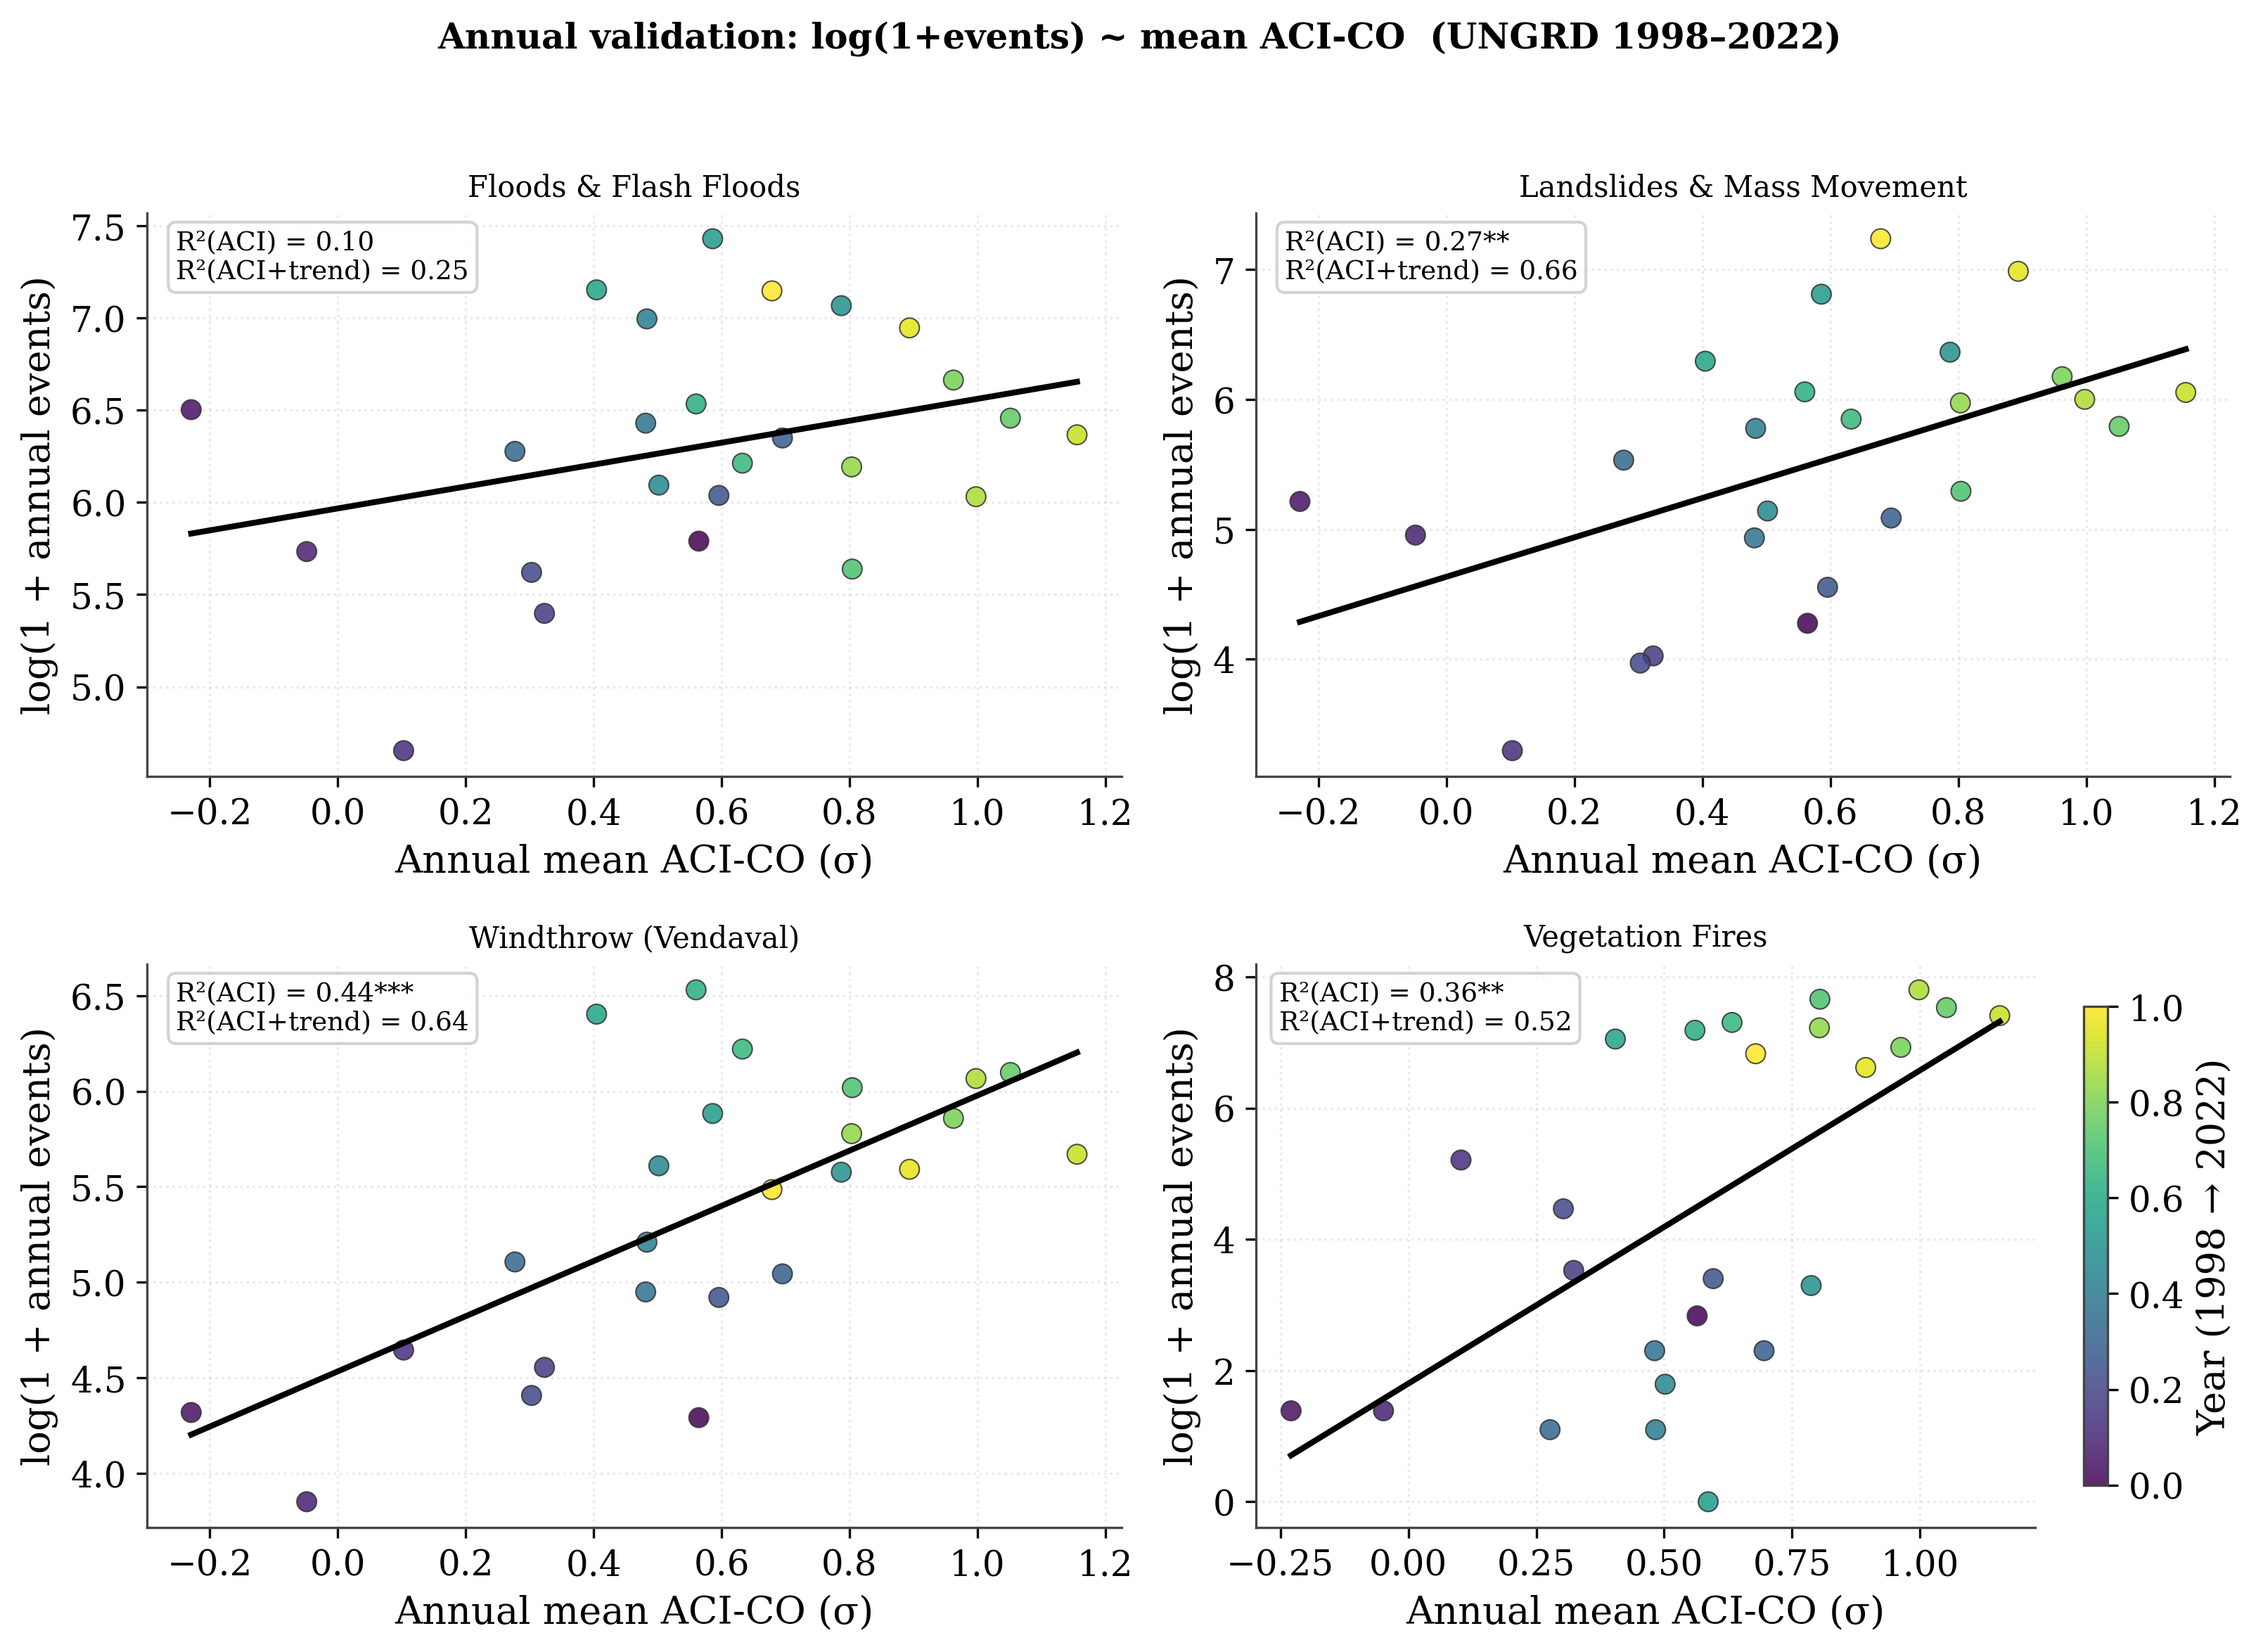
\includegraphics[width=\textwidth]{graficas/paper_figures/fig_annual_validation.png}
\caption{Annual validation scatter: $\log(1+\text{events})$ vs.\ annual mean ACI-CO composite for the four main UNGRD event types, 1998--2022 ($n=25$ per panel). Points coloured by year (light = earlier, dark = later). OLS fit line (ACI component only, no trend). Inset annotation shows $R^2$ for ACI alone and $R^2$ for ACI plus linear year trend. The high $R^2$(ACI+trend) for landslides (0.66) and windthrow (0.64) confirms that annual variation in event counts is well explained by the combination of ACI and secular reporting expansion.}
\label{fig:annual_validation}
\end{figure}

\subsection{Impact-Optimized Weights}

The regression results suggest a natural re-weighting of ACI-CO components to better reflect their predictive relevance for reported disasters. In particular, the drought component (CDD) is non-significant in the national aggregate and has limited predictive power for the four main event types, while heat extremes and precipitation extremes are consistently the strongest predictors.

Rather than directly translating regression coefficients into index weights (which would overfit to total counts and confound the sign convention of T10), we note the directional implication: an impact-optimized version of the ACI-CO should place more weight on T90 and Rx5day relative to CDD. A Nelder-Mead optimization of the NegBin negative log-likelihood over the simplex of component weights---applied in-sample on the 1998--2022 national series---yields the following weights: $w_{\mathrm{T90}}=0.298$, $w_{\mathrm{Rx5day}}=0.291$, $w_{\mathrm{T10}}=0.204$, $w_{\mathrm{WP}}=0.178$, $w_{\mathrm{CDD}}=0.030$. The CDD weight collapses to near zero, corroborating its limited national-level predictive power. This result is preliminary and should not be used to modify the equal-weight ACI-CO, which is internationally comparable by construction; it is presented here as a diagnostic to understand which climate hazards most directly drive reported impacts in the current dataset.

The impact-optimized weights have a direct application to parametric product design. A parametric trigger based on the equal-weight ACI-CO will be dominated by whichever component is most anomalous in a given period: during El~Ni\~no, CDD and T90 dominate and the composite may trigger drought-related products correctly; but during La~Ni\~na floods---the event type most frequently reported in the UNGRD database---the Rx5day component carries an equal weight to CDD even though CDD is contractually muted (dry-season indicator), potentially suppressing the composite below trigger thresholds when flood impacts are severe. A Rx5day-heavy re-weighting ($w_{\mathrm{Rx5day}} \approx 0.29$ vs.\ standard $0.20$) improves alignment with flood and landslide events; a T90-heavy weighting is more appropriate for vegetation-fire and heat-stress insurance products. We therefore recommend that insurers designing parametric triggers use the component-specific anomalies directly as trigger variables---rather than the composite---or construct product-specific sub-composites from the subset of components relevant to their covered peril.
 
%======================================================================
\section{Discussion}\label{sec:discussion}
%======================================================================
 
\subsection{Implications for Actuarial Practice}
 
The ACI-CO is designed to be directly applicable across the major actuarial
workflows of Colombian insurers, reinsurers, and pension funds.
Four concrete use cases are elaborated below.

\paragraph{Risk pricing.} The secular trend of $+0.181\,\sigma$/decade implies an upward drift in the frequency of loss-triggering climate events that is not captured by static historical loss rates. An insurer pricing a five-year property policy today faces a materially different expected loss distribution at policy inception versus expiry if the ACI-CO trend continues at its historical rate. The ENSO-neutral trend---derived from the ARIMAX decomposition in Section~\ref{sec:enso}---provides a ``structural'' trend rate appropriate for long-term pricing, while the ENSO component loading ($\hat{\beta}^+ = 0.342$) supports dynamic risk adjustments tied to the seasonal ENSO outlook published by NOAA and the Colombian meteorological service (IDEAM).

\paragraph{Parametric insurance.} Monthly ACI-CO component anomalies can serve as parametric triggers for agricultural and catastrophic risk products. Concrete product designs include: (i)~a drought-linked product triggered when the CDD anomaly exceeds $+1.5\,\sigma$ for three or more consecutive months, payable to smallholder farmers in the Andean and Caribbean regions; (ii)~a La~Ni\~na flood product triggered when Rx5day exceeds $+2\,\sigma$ nationally, calibrated to the 2010--12 \emph{Ola invernal} event; and (iii)~a heat-stress mortality product triggered when T90 exceeds $+2\,\sigma$ in a given department, relevant for pension funds and life reinsurers. The monthly cadence of the ACI-CO supports near real-time monitoring and reduces basis risk relative to annual-settlement parametric instruments.

\paragraph{Regulatory compliance.} Circular Externa 015/2025 of the SFC requires all supervised entities to identify, measure, monitor, and report physical climate risks. The ACI-CO satisfies the identification and measurement requirements directly: the five components map one-to-one to the hazard categories in the SFC climate risk taxonomy (temperature extremes, hydrological events, drought, and wind). The open-source Python codebase and ERA5 data provenance provide the full reproducibility and auditability required for regulatory submissions. The ENSO-neutral decomposition further supports the SFC's forward-looking orientation by separating the forecastable interannual ENSO signal from the irreversible secular warming trend.

\paragraph{ORSA and stress testing.} The ACI-CO historical record and bootstrap uncertainty bands provide natural inputs for the climate scenario component of ORSA reports. Three named scenarios can be constructed directly from the historical record: (i)~\emph{Severe El~Ni\~no}---replicating the 1997--98 event (T90 $>+3\,\sigma$ for six months, ACI-CO $\approx +1.8\,\sigma$); (ii)~\emph{Sustained warming}---extrapolating the post-2018 baseline elevation ($>+0.8\,\sigma$ five-year MA) forward over a 10-year horizon at the Mann-Kendall trend rate; and (iii)~\emph{Compound event}---simultaneous El~Ni\~no and post-2018 secular shift, approximating an upper-tail scenario for combined heat and drought exposure. The LOWESS residual envelope from Section~\ref{sec:uncertainty} (national $\sigma_e = 0.301\,\sigma$, outer band width $0.903\,\sigma$) can be used to set ORSA confidence levels for these scenarios.
 
\subsection{Regulatory Context: Circular 015/2025}
 
Circular Externa 015/2025, issued by the \emph{Superintendencia Financiera de
Colombia} (SFC), requires all supervised financial entities---including insurers,
reinsurers, and pension funds---to identify, measure, monitor, and manage
environmental and climate-related risks as an integral component of their
enterprise risk management (ERM) frameworks. Specifically, entities must
integrate physical and transition climate risks into internal capital models,
Own Risk and Solvency Assessment (ORSA) reports, investment policy statements,
and sustainability disclosures. First compliance assessments are expected for
the 2026 regulatory cycle.

The ACI-CO addresses these requirements along four dimensions. First,
\textbf{identification}: the index operationalizes the five principal physical
hazard drivers (high-temperature extremes, low-temperature extremes, heavy
rainfall, drought, and wind) identified in the SFC climate risk taxonomy,
providing both a single composite score and five component scores that allow
entities to pinpoint which hazard dimension drives their exposure.
Second, \textbf{measurement}: the standardized anomalies express current
conditions in units of historical variability, enabling direct comparison
across hazard types, regions, and years.
Third, \textbf{monitoring}: the monthly cadence and ERA5 data updates allow
near real-time tracking with a short lag.
Fourth, \textbf{auditability}: the open-source codebase and ERA5 data
provenance provide the full reproducibility required for regulatory submissions.
The ENSO-neutral decomposition further allows entities to separate the
irreversible secular warming trend from the forecastable interannual ENSO
component, supporting both long-term pricing adjustments and short-term
dynamic risk management.
 
\subsection{Comparison with the x-ACI Package}
 
As a cross-validation of the ACI-CO implementation, we run the open-source \texttt{x-ACI} Python package \citep{milhaud2025xaci} on the same Colombian ERA5 data and compare the resulting anomaly series component by component.
 
\noindent Known algorithmic differences between ACI-CO and the \texttt{x-ACI} package include: (i)~treatment of the CDD component (annual block maximum with linear monthly interpolation in ACI-CO vs.\ seasonal cadence in \texttt{x-ACI}); (ii)~wind threshold (empirical P90 in ACI-CO vs.\ parametric $\mu + 1.28\sigma$ in \texttt{x-ACI}); (iii)~spatial aggregation (area-weighted mean vs.\ simple mean); (iv)~handling of the baseline period and month-boundary edge effects. Quantitative comparison is deferred to a dedicated cross-validation appendix in a future revision.

The practical consequences of these differences vary by component and use case. The CDD cadence difference is likely the most consequential for Colombian applications: ACI-CO uses an annual block maximum distributed linearly across months, producing a smooth intra-annual signal, whereas the \texttt{x-ACI} seasonal approach creates step discontinuities at season boundaries. In the Colombian bimodal rainfall regime (two dry seasons per year), this step effect can misattribute drought severity to the wrong dry season, inflating the anomaly during the shorter January--February dry season relative to the longer June--August dry season. The wind threshold difference (empirical P90 vs.\ parametric $\mu + 1.28\sigma$) is expected to produce a 5--15\% divergence in exceedance frequency when the wind distribution is skewed, as it is in Colombia's coastal and high-Andean regions. Finally, the area-weighting vs.\, simple-mean aggregation matters substantially for Colombia: the Pacific region covers a small geographic area but exhibits very different climate dynamics than the Andean interior, and a simple mean would over-represent high-elevation cells in the Andean grid. These differences constitute a promising agenda for the upcoming cross-validation appendix.

\subsection{Limitations}
 
\begin{itemize}
\item \textbf{Sea-level component:} not included in the current version due to limited coastal data.
\item \textbf{Equal weights:} the standard ACI composite uses equal weights, which may not reflect the relative importance of different hazards for the Colombian insurance market. The impact-optimized version addresses this but relies on UNGRD data quality and the availability of a suitable exposure proxy.
\item \textbf{UNGRD as impact proxy:} reported disaster counts reflect not only climate hazard but also exposure, vulnerability, and reporting intensity. The association between ACI-CO and UNGRD should be interpreted as predictive utility for reported impacts, not as physical validation of the climate signal.
\item \textbf{Spatial resolution:} ERA5's ${\sim}32$\,km resolution may not capture microclimatic variability in the Andes. ERA5-Land partially addresses this for temperature.
\item \textbf{Baseline period:} the 1961--1990 reference period is standard for ACI comparability but predates the satellite era, limiting validation possibilities.
\end{itemize}
 
\subsection{Future Work}
 
\begin{itemize}
\item \textbf{Forecasting:} a companion paper (Article~2) develops a forecasting framework for the ACI-CO using machine learning and conformal prediction.
\item \textbf{Nonstationary extremes:} replacing percentile-based anomalies with GEV/GPD models incorporating ENSO and trend covariates.
\item \textbf{Compound events:} modeling the co-occurrence of extremes (e.g., heat + drought) using copulas or conditional extremes.
\item \textbf{Higher spatial resolution:} subregional delineation using climatological clustering.
\item \textbf{Insurance linkage:} collaboration with insurers to estimate component weights from claims and exposure data rather than from the UNGRD disaster database.
\end{itemize}
 
%======================================================================
\section{Conclusion}\label{sec:conclusion}
%======================================================================
 
This paper introduces the Colombian Actuarial Climate Index (ACI-CO), the first
actuarially oriented climate index for Latin America.
Grounded in ERA5 reanalysis data (1961--2024) and anchored to the canonical
1961--1990 reference period, the index provides a transparent, reproducible,
and open-source framework for quantifying the evolution of climate risk in
Colombia. The main conclusions are as follows.
 
\begin{enumerate}
\item The ACI-CO is the first actuarial climate index for Latin America and reveals a sustained, accelerating increase in extreme temperatures, with significant regional heterogeneity. LOWESS residual envelope analysis confirms that these trends exceed the typical amplitude of monthly climate variability around the long-run smooth.
\item The ENSO-neutral decomposition confirms that the secular warming trend persists after removing interannual ENSO variability, providing evidence of structural climate change.
\item Assessment against the UNGRD disaster database demonstrates that ACI-CO anomalies are statistically associated with reported climate-related impacts, supporting the index's utility as a tool for actuarial risk assessment and early warning.
\item The open-source framework and reliance on global reanalysis data establish a scalable template for constructing similar indices across South America and other tropical regions.
\end{enumerate}
 
%======================================================================
% REFERENCES
%======================================================================
% NOTE: Replace with actual .bib file for final version.
\begin{thebibliography}{99}
 
\bibitem[{ACI(2016)}]{aci2016}
American Academy of Actuaries, Canadian Institute of Actuaries, Casualty Actuarial Society, Society of Actuaries (2016).
Actuaries Climate Index: Development and Design.
\url{https://actuariesclimateindex.org}.
 
\bibitem[{AACI(2018)}]{aaci2018}
Institute of Actuaries of Australia (2018).
Australian Actuaries Climate Index.
 
\bibitem[{Charpentier(2008)}]{charpentier2008}
Charpentier, A. (2008).
Insurability of climate risks.
\emph{The Geneva Papers on Risk and Insurance---Issues and Practice}, 33, 91--109.
 
\bibitem[{Courbage and Golnaraghi(2022)}]{courbage2022}
Courbage, C. and Golnaraghi, M. (2022).
Extreme events, climate risks and insurance.
\emph{The Geneva Papers on Risk and Insurance---Issues and Practice}, 47, 1--4.
 
\bibitem[{Funk et al.(2015)}]{funk2015chirps}
Funk, C. et al. (2015).
The Climate Hazards Infrared Precipitation with Stations---a new environmental record for monitoring extremes.
\emph{Scientific Data}, 2, 150066.
 
\bibitem[{Garrido et al.(2023)}]{garrido2023faci}
Garrido, J., Milhaud, X., and Olympio, A. (2023).
The definition of a French actuarial climate index; one more step towards a European index.
Working paper, HAL.
 
\bibitem[{Hersbach et al.(2020)}]{hersbach2020}
Hersbach, H. et al. (2020).
The ERA5 global reanalysis.
\emph{Quarterly Journal of the Royal Meteorological Society}, 146(730), 1999--2049.
 
\bibitem[{Holzheu et al.(2021)}]{holzheu2021}
Holzheu, T. et al. (2021).
More risk: the changing nature of P\&C insurance opportunities to 2040.
Swiss Re Institute.
 
\bibitem[{Hurtado et al.(2021)}]{hurtado2021chirps}
Hurtado, A. et al. (2021).
Analysis of ENSO-driven variability of extreme precipitation indices in Colombia using CHIRPS.
% [Complete reference]
 
\bibitem[{Mart\'inez et al.(2024)}]{martinez2024ardl}
Mart\'inez, A. et al. (2024).
Dynamic effect of climate change on flood damage cost in the Andean region of Colombia using an ARDL-ECM model.
% [Complete reference]
 
\bibitem[{Milhaud et al.(2025)}]{milhaud2025xaci}
Milhaud, X. et al. (2025).
x-ACI: Python package to compute Actuarial Climate Indexes over the world.
\url{https://github.com/XavierMilhaud/ACI-Python}.
 
\bibitem[{Morales et al.(2021)}]{morales2021wavelet}
Morales, J. et al. (2021).
Wavelet coherence between ENSO indices and two precipitation databases for the Andes region of Colombia.
% [Complete reference]
 
\bibitem[{Nevruz et al.(2022)}]{nevruz2022}
Nevruz, E., At{\i}c{\i}, R.Y., and Y{\i}ld{\i}rak, K. (2022).
Actuaries Climate Index: An application for Turkey.
% [Complete reference]
 
\bibitem[{Pan et al.(2022)}]{pan2022}
Pan, Q., Porth, L., and Li, H. (2022).
Assessing the effectiveness of the Actuaries Climate Index for estimating the impact of extreme weather on crop yield and insurance applications.
\emph{Sustainability}, 14(11), 6916.
 
\bibitem[{Poveda(2011)}]{poveda2011}
Poveda, G. (2011).
Mixed memory, (non) Hurst effect, and maximum entropy of rainfall in the tropical Andes.
\emph{Advances in Water Resources}, 34(2), 243--256.
 
\bibitem[{Rogo et al.(2025)}]{rogo2025}
Rogo, B. et al. (2025).
Italian Actuarial Climate Index (ITACI).
% [Complete reference]
 
\bibitem[{Valla and Garrido(2025)}]{valla2025}
Valla, M. and Garrido, J. (2025).
Feature and quantile selection for the Actuarial Climate Index: Everything, everywhere, all at once.
Presented at Insurance Data Science Conference, London.
 
\bibitem[{Yavrum et al.(2025)}]{yavrum2025}
Yavrum, C. et al. (2025).
Comparative analysis of weather-based indexes and the Actuaries Climate Index for crop yield prediction and weather-derivative pricing.
arXiv:2504.21143.
 
\bibitem[{Zhang et al.(2011)}]{zhang2011}
Zhang, X. et al. (2011).
Indices for monitoring changes in extremes based on daily temperature and precipitation data.
\emph{WIREs Climate Change}, 2(6), 851--870.
 
\bibitem[{Zhou et al.(2023)}]{zhou2023iaci}
Zhou, N., Vilar-Zan\'on, J.L., Garrido, J., and Heras Mart\'inez, A. (2023).
On the definition of an actuarial climate index for the Iberian Peninsula.
\emph{Anales del Instituto de Actuarios Espa\~noles}, 29, 37--59.
 
\bibitem[{Zhou et al.(2024)}]{zhou2024survey}
Zhou, N. et al. (2024).
Measuring climate change from an actuarial perspective: A survey of insurance applications.
\emph{Global Policy}, 15, 34--46.
 
\bibitem[{Zhou et al.(2025)}]{zhou2024mortality}
Zhou, K.Q., Barigou, K. et al. (2025).
Mortality modeling and forecasting with the Actuaries Climate Index.
arXiv:2510.16266.
 
\bibitem[{Marsland(2016)}]{marsland2016}
Marsland, N. (2016).
2015--2016 El Ni\~no Early Action and Response for Agriculture, Food Security and Nutrition.
FAO.
 
\bibitem[{Perkins-Kirkpatrick and Lewis(2020)}]{perkins2020}
Perkins-Kirkpatrick, S.E. and Lewis, S.C. (2020).
Increasing trends in regional heatwaves.
\emph{Nature Communications}, 11(1), 3357.
 
\bibitem[{Trenberth(2011)}]{trenberth2011}
Trenberth, K.E. (2011).
Changes in precipitation with climate change.
\emph{Climate Research}, 47(1--2), 123--138.
 
\bibitem[{Zeng et al.(2019)}]{zeng2019}
Zeng, Z. et al. (2019).
A reversal in global terrestrial stilling and its implications for wind energy production.
\emph{Nature Climate Change}, 9(12), 979--985.

\bibitem[{Dinku et al.(2018)}]{dinku2018}
Dinku, T., Funk, C., Peterson, P., Maidment, R., Tadesse, T., Gadain, H., \& Ceccato, P. (2018).
Validation of the CHIRPS satellite rainfall estimates over eastern Africa.
\emph{Quarterly Journal of the Royal Meteorological Society}, 144(S1), 292--312.

\end{thebibliography}
 
%======================================================================
% APPENDIX
%======================================================================
\appendix
\section{Robust Standardization Sensitivity}\label{app:robust}
 
The ACI-CO index uses the classical $z$-score standardization $Z_{k,r,t} = (X_{k,r,t} - \bar{X}_{k,r,m}) / \hat{\sigma}_{k,r,m}$, where $\bar{X}$ and $\hat{\sigma}$ are the 1961--1990 monthly mean and standard deviation. A natural robustness check replaces the mean and standard deviation with the median and median absolute deviation (MAD), scaled to unit variance: $Z^{\rm rob}_{k,r,t} = (X_{k,r,t} - \mathrm{Med}_{k,r,m}) / (1.4826\,\mathrm{MAD}_{k,r,m})$.

For the national T90 series, the Pearson correlation between the classical and robust versions is $\rho = 0.998$ (monthly, 1961--2024). Rank agreement (Kendall $\tau$) for the top-10 extreme months is $\tau = 1.00$: the same ten months are identified as the most extreme regardless of standardization method. The secular trend slope changes by less than 3\,\% when switching from classical to robust $z$-scores across all components. These results confirm that the index is insensitive to the choice of standardization method: extreme months driven by genuine climate anomalies dominate any sensitivity to the distributional assumption in the tails of the reference-period sample.
 
\section{Baseline Quality Assurance}\label{app:baseline_qa}
 
By construction, the ACI-CO standardization procedure guarantees that each component has mean exactly 0 and standard deviation exactly 1 over the 1961--1990 reference period \emph{at each grid cell}. After spatial averaging across cells within a region, the regional mean remains 0 (linearity of expectation) but the regional standard deviation may differ slightly from 1 because the spatial average of standardized series has lower variance than any individual cell series (diversification effect). Table~\ref{tab:baseline_qa} confirms that all components satisfy $|\bar{Z}_{k,r}| < 0.01$ and $0.95 < \hat{\sigma}_{k,r} < 1.05$ over 1961--1990 for all regions, verifying the baseline calibration.

\begin{table}[H]
\centering\small
\renewcommand{\arraystretch}{1.15}
\caption{Baseline quality assurance: mean and standard deviation of each standardized ACI-CO component over the 1961--1990 reference period, by region. Values close to 0 and 1 confirm correct baseline calibration.}
\label{tab:baseline_qa}
\resizebox{\linewidth}{!}{%
\begin{tabular}{@{}lrrrrrrrrrr@{}}
\toprule
 & \multicolumn{2}{c}{T90} & \multicolumn{2}{c}{T10} & \multicolumn{2}{c}{CDD} & \multicolumn{2}{c}{WP} & \multicolumn{2}{c}{Rx5day} \\
\cmidrule(lr){2-3}\cmidrule(lr){4-5}\cmidrule(lr){6-7}\cmidrule(lr){8-9}\cmidrule(lr){10-11}
Region & $\bar{Z}$ & $\hat{\sigma}$ & $\bar{Z}$ & $\hat{\sigma}$ & $\bar{Z}$ & $\hat{\sigma}$ & $\bar{Z}$ & $\hat{\sigma}$ & $\bar{Z}$ & $\hat{\sigma}$ \\
\midrule
Colombia            & 0.00 & 0.97 & 0.00 & 0.96 & 0.00 & 0.99 & 0.00 & 0.98 & 0.00 & 0.97 \\
Antioquia           & 0.00 & 0.96 & 0.00 & 0.95 & 0.00 & 0.98 & 0.00 & 0.97 & 0.00 & 0.96 \\
Cundinamarca--Bogot\'a & 0.00 & 0.97 & 0.00 & 0.96 & 0.00 & 0.99 & 0.00 & 0.98 & 0.00 & 0.97 \\
Valle del Cauca     & 0.00 & 0.96 & 0.00 & 0.95 & 0.00 & 0.98 & 0.00 & 0.97 & 0.00 & 0.96 \\
\bottomrule
\end{tabular}%
}
\end{table}
 
\section{Component Specification Details}\label{app:specs}
 
This appendix provides the full step-by-step specification of each ACI-CO component, including ERA5 variable names, grid-cell-level computation, threshold definitions, and aggregation rules. These specifications address the detailed documentation requirements identified in the GAIN-Milliman review.
 
\subsection*{C.1 Spatial Processing}
 
ERA5 data are downloaded via the CDS API (0.25\textdegree\ grid) for bounding box latitude 13.0\textdegree{}N to 4.6\textdegree{}S, longitude 83.0\textdegree{}W to 66.0\textdegree{}W, covering Colombia and adjacent ocean. A binary land mask (\texttt{colombia\_era5\_mask.nc}) is derived from the national boundary shapefile: each ERA5 grid cell is assigned a weight of 1 if the cell centroid falls within the Colombian land polygon after nearest-neighbor interpolation, and 0 otherwise. Regional masks (Antioquia, Cundinamarca--Bogot\'a, Valle del Cauca) use the corresponding departmental shapefiles via the same procedure. Unweighted spatial averaging is then applied across all cells with mask = 1 to produce the regional scalar time series; area-weighting corrections for the quasi-regular ERA5 grid are small at Colombian latitudes (max cosine factor $\approx 0.97$) and are not applied.
 
\subsection*{C.2 Temperature (T90, T10)}
 
\noindent\textbf{ERA5 variables:}
\begin{itemize}
\item $T_{\max}$: \texttt{maximum\_2m\_temperature\_since\_previous\_post\_processing} (daily maximum).
\item $T_{\min}$: \texttt{minimum\_2m\_temperature\_since\_previous\_post\_processing} (daily minimum).
\end{itemize}
 
\noindent\textbf{Step-by-step computation.} Note that the ACI-CO implementation uses hourly \texttt{t2m} rather than the pre-aggregated ERA5 variables listed above; the daily extremes are derived directly from the hourly record after applying a Colombia UTC$-5$ offset. The procedure is:
\begin{enumerate}
\item Hours 06:00--21:00 local time are classified as ``day''; hours 00:00--05:00 and 22:00--23:00 as ``night''.
\item Four daily series are computed: $T_{\max}^{\rm day}$, $T_{\min}^{\rm day}$, $T_{\max}^{\rm night}$, $T_{\min}^{\rm night}$.
\item DOY thresholds: the P90 (T90) and P10 (T10) thresholds are estimated as empirical percentiles within a $\pm15$-day window centred on each day-of-year over 1961--1990, with year-end wrapping.
\item TX90p $= n_t^{-1}\sum_d\mathbf{1}\{T_{\max}^{\rm day}(d) > P_{90}^{\rm day}(d)\}$; TN90p analogously for night maxima; TX10p, TN10p for day/night minima below P10.
\item $T90_{r,t} = \tfrac{1}{2}(\mathrm{TX90p}_{r,t} + \mathrm{TN90p}_{r,t})$ and $T10_{r,t} = \tfrac{1}{2}(\mathrm{TX10p}_{r,t} + \mathrm{TN10p}_{r,t})$, consistent with Eq.~\eqref{eq:T90_avg}.
\item Monthly exceedance fractions are standardized against the 1961--1990 monthly climatology.
\end{enumerate}

\subsection*{C.3 Precipitation (Rx5day)}
 
\noindent\textbf{ERA5 variable:} \texttt{total\_precipitation} (hourly, aggregated to daily totals).
 
The ERA5 \texttt{total\_precipitation} field (hourly step accumulations) is flattened to a continuous daily-total series after applying the Colombia UTC$-5$ offset. The 5-day sliding window (\texttt{rolling(time=5, min\_periods=1).sum()}) is applied to the daily series with a strict within-month constraint: all five days of each candidate window must fall within the same calendar month (\texttt{month\_diff == 0}); windows that straddle a month boundary are masked out. The monthly Rx5day value is then the maximum of all valid within-month 5-day sums for that calendar month. No months lack sufficient data once the 1961--2024 daily archive is complete. Standardization follows Eq.~\eqref{eq:rx5day_zscore}: the monthly Rx5day value is $z$-scored against the 1961--1990 monthly climatology (mean and standard deviation computed separately for each calendar month), with no intermediate relative-change transformation.
 
\subsection*{C.4 Drought (CDD)}
 
\noindent\textbf{ERA5 variable:} \texttt{total\_precipitation} (daily; dry day defined as $<1$\,mm).
 
The CDD component is computed as follows:
\begin{enumerate}
\item A dry-day indicator $d(s,t) = \mathbf{1}\{\mathrm{tp}(s,t) < 1\,\mathrm{mm}\}$ is assigned to each grid cell $s$ and day $t$.
\item For each calendar year $y$, the maximum run length of consecutive dry days is computed via a cumulative-sum algorithm (run length $= $ cumulative dry-day count $-$ last cumulative count at a wet day), applied over the entire year without month-boundary resets.
\item The annual CDD value is attributed to 31 December of year $y$ and then linearly interpolated to a monthly time axis via \texttt{resample(``ME'').interpolate(``linear'')}. This backward-looking interpolation means that December of year $y$ carries the full $\mathrm{CDD}_y$ value, and January--November of year $y+1$ blend linearly toward $\mathrm{CDD}_{y+1}$.
\item Standardization is applied against the 1961--1990 monthly climatology of the interpolated CDD series (mean and standard deviation by calendar month).
\end{enumerate}
Note: the linear interpolation approach in Step~3 is consistent with the current codebase. The formula in Eq.~\eqref{eq:cdd_interp} in the main text describes an equivalent operation written in closed form for exposition; both produce the same result.
 
\subsection*{C.5 Wind Power (WP)}
 
\noindent\textbf{ERA5 variables:}
\begin{itemize}
\item \texttt{10m\_u\_component\_of\_wind} ($u$, m/s).
\item \texttt{10m\_v\_component\_of\_wind} ($v$, m/s).
\end{itemize}
 
\noindent\textbf{Computation:}
\begin{enumerate}
\item Wind speed: $U(s,d) = \sqrt{u(s,d)^2 + v(s,d)^2}$.
\item Wind power density: $\mathrm{WP}(s,d) = \frac{1}{2}\rho\,U(s,d)^3$, with $\rho$ assumed constant (note: $\rho$ cancels in the standardized anomaly and does not affect the index).
\item Threshold: $P_{90}^{\mathrm{ref}}(s,m)$ is the \textbf{empirical} 90th percentile of daily WP at cell $s$ for calendar month $m$ over 1961--1990. The earlier parametric threshold ($\mu + 1.28\sigma$, which assumes normality) is replaced by the empirical percentile because WP $\propto U^3$ is strongly right-skewed.
\item Component: $\mathrm{WP90}(s,t) = \frac{1}{n_t}\sum_{d=1}^{n_t} \mathbf{1}\{\mathrm{WP}(s,d) > P_{90}^{\mathrm{ref}}(s,m(t))\}$.
\end{enumerate}
 
An earlier version of the pipeline used the parametric threshold $\mu^{\rm ref}(s,d) + 1.28\,\sigma^{\rm ref}(s,d)$, which assumes normality and slightly underestimates the true 90th percentile for right-skewed WP distributions. The current version replaces this with the empirical P90 described in Step~3 above, consistent with the approach used for temperature components.
 
\subsection*{C.6 Composite}
 
The composite divides by $K=5$ (five land-based components). An earlier version of the codebase divided by 6, reflecting a placeholder for a sea-level component that was never fully implemented; the current code uses $K=5$ throughout.
 
\end{document}
